%# -*- coding:utf-8 -*-
%!TEX program = xelatex
\documentclass[twoside,AutoFakeBold=true]{ZJUthesis}
% 该文档中首字符为“%”的均为注释行,不会在论文中出现
% https://github.com/shuwei1204/ZJUthesis
% https://github.com/KwenString/Thesis-SE-ZJU-LaTeX

% AutoFakeBold=true 是为解决在Windows系统下,使用xelatex时中文字体不能加粗的问题

% 取消目录中链接的颜色,方便打印
% 如需颜色,请将“false”改为“true”
\hypersetup{colorlinks=false}
%\usepackage{ccmap} %解决生成pdf的中文复制文字后乱码问题
%\usepackage[sectionbib]{chapterbib}
\usepackage[chapter]{algorithm}
\floatname{algorithm}{算法}
\usepackage{paralist}
\usepackage{algorithmic}
\usepackage{tabularx}
\usepackage{multirow}
\usepackage{cleveref}
\usepackage{adjustbox}
\usepackage{tikz}
\usepackage{pgfplots}
\pgfplotsset{compat=1.10}
\usepgfplotslibrary{colormaps}
\usetikzlibrary{pgfplots.colormaps}

\usepackage{caption}
\usepackage{wrapfig}

\renewcommand{\algorithmicrepeat}{\textbf{重复}}
\renewcommand{\algorithmicuntil}{\textbf{直到}}
\renewcommand{\algorithmicfor}{\textbf{对于}}
\renewcommand{\algorithmicdo}{\textbf{}}
\renewcommand{\algorithmicend}{\textbf{结束}}

\newcommand{\crefrangeconjunction}{至}
\newcommand{\crefpairconjunction}{和}
\newcommand{\creflastgroupconjunction}{和}
\crefname{figure}{图}{图}
\crefname{equation}{公式}{公式}
\crefname{table}{表}{表}
\crefname{algorithm}{算法}{算法}
\crefname{chapter}{章}{章}


\begin{document}
\fangsong\zihao{-4} %% 正文字体设定
%%%%%%%%%%%%%%%%%%%%%%%%%%%%%%%
%%% 中文封面内容
%%%%%%%%%%%%%%%%%%%%%%%%%%%%%%%
\classification{TP391.41}% 中图分类号
\serialnumber{10335}% 单位代码
\SecretLevel{无}% 密级
\PersonalID{11521059}%

\title{面向复杂场景理解的视觉内容识别、}%中文题目
\titletl{检测与推理方法研究}

\Etitle{Visual Recognition, Detection, and Reasoning}%英文题目
\Etitletl{for Complex Visual Scene Understanding}

\author{陈隆}%

\degree{博士}

\supervisor{肖俊}%
\cpsupervisor{}%
\major{计算机科学与技术}% 专业名称
\researchdm{计算机视觉}
\institute{计算机科学与技术学院}

\submitdate{2020 年 xx 月 xx 日}
\defenddate{2020 年 xx 月 xx 日}
\defenddateE{xx June 2020}


%%%%%%%%%%%%%%%%%%%%%%%%%%%%%%
%% 中文题名页内容
%%%%%%%%%%%%%%%%%%%%%%%%%%%%%%
% 论文评阅人信息 注意两字名与三字名,两字职称与三字职称的写法,便于对齐
% 多余的名额直接注释掉即可,比如三个评阅人,把评阅人D,E注释掉即可
\reviewersA{}%(隐名评阅学位论文省略)
\reviewersB{}
\reviewersC{}
\reviewersD{}
\reviewersE{}

% 答辩委员会信息,如果某一个单位比较长,
% 请在其它较短后面补上{hspace{Xem}},X是比最长的单位名少几个字
% 如果实际人数少于6人,多余的注释掉即可
\chairman{ xx   \quad\quad 教授	\quad\quad xx大学} 
\commissionerA{xx	\quad\quad 教授	\quad\quad xx大学}
\commissionerB{xx	\quad\quad 教授	\quad\quad xx大学} %计算机科学与技术学院
\commissionerC{xx	\quad\quad 教授	\quad\quad xx大学}
\commissionerD{xx	\quad\quad 教授	\quad\quad xx大学}



%%%%%%%%%%%%%%%%%%%%%%%%%%%%%%
%% 英文题名页内容
%%%%%%%%%%%%%%%%%%%%%%%%%%%%%%

% 评阅人信息,名字,职称,单位尽量用简写,否则会写不下
\EreviewersA{}
\EreviewersB{}
\EreviewersC{}
\EreviewersD{}
\EreviewersE{}

% 答辩委员会信息,同样尽量用简写,否则会写不下
\Echairman{}
\EcommissionerA{}
\EcommissionerB{}
\EcommissionerC{}
\EcommissionerD{}
%\EcommissionerD{xx	\hspace{1em}\quad\quad Professor	\quad ZJU}




%%%%%%%%%%%%%%%%%%%%%%%%%%%%%%
%% 原创声明与版权协议页
%%%%%%%%%%%%%%%%%%%%%%%%%%%%%%

\SignautreDateA{}{}{}
\SignautreDateB{}{}{}
\SignautreDateC{}{}{}

%%%%%%%%%%%%%%%%%%%%%%%%%%%%%%
%% 论文部分开始
%%%%%%%%%%%%%%%%%%%%%%%%%%%%%%


%%%%%%%%%%%%%%%%%%%%%%%%%%%%%%
\makeCoverPage% 生成封面
\maketitle	% 生成中文题名页
\makeenglishtitle	% 生成英文封面
\makeOSandCPRTpage	% 生成原创声明与版权协议页
%%%%%%%%%%Roman page numbering%%%%%%%%
\ZJUfrontmatter
%# -*- coding:utf-8 -*-
\begin{abstract}

尽管近年来计算机视觉技术已经取得了长足的进步,但是对于复杂视觉场景的感知和理解,目前的计算机模型表现远远没有达到大规模普及和落地应用的水平。为了充分地利用日常生活中海量的视觉媒体数据,复杂视觉场景的感知和理解已经逐渐成为计算机视觉领域的一个研究热点。

本文将针对四个不同层次的视觉场景理解(物体识别、场景识别、场景理解和场景推理),逐步地对复杂视觉场景中视觉内容的识别、检测和推理进行研究。本文的关键技术线路主要聚焦于零样本物体分类、图像场景图生成、图像描述生成、视频片段检索和视觉问答等具体视觉场景理解任务。在此研究技术路线下,本文主要的研究内容和贡献如下:

1)针对零样本物体分类模型中普遍存在的语义丢失的问题,本文提出一种全新的零样本学习网络。该网络首次引入两个相互独立的映射网络分支,将图像分类和图像重建两个原本相互冲突的任务分离出来。同时借助对抗学习,实现重建网络分支和分类网络分支之间的属性迁移。

2)针对图像场景图生成模型中优化目标通常忽略不同物体的重要性差异的问题,本文提出一种全新的训练框架,首次将场景图生成任务转化成多智能体协同决策问题,从而可以直接将整个场景图质量作为模型的优化目标。同时,本文还提出了一种反事实基准模型,可以有效地计算每个物体类别预测对整体场景图的局部贡献。

3)参考现有的空间注意力机制,本文首次提出通道注意力机制。同时,通过充分挖掘卷积神经网络的特征图的三个不同维度(空间、通道和层级)之间的联系,提出一种全新的空间和通道注意力网络。在图像描述生成任务中,该网络不仅极大地提升了描述语句的生成质量,同时帮助人们理解在语句生成过程中特征图的变化过程。

4)针对目前视频片段检索任务中两种主流框架(自顶向下和稀疏型自底向上)的设计缺陷,本文提出了一种全新的密集型自底向上的框架。通过将动作边界定位问题分解成相关性预测和边界回归两个子问题,显著地降低了动作边界定位的难度。同时,本文提出一个基于图卷积的特征金字塔层,来进一步增强骨干网络编码能力。

5)针对目前视觉问答模型忽略的两个重要特性(视觉可解释性和问题敏感性),本文提出了一种通用的反事实样本生成机制。通过遮盖图像中的重要区域或问题中的重要单词,同时更改标准答案,来合成反事实样本。通过使用原始样本和反事实样本一起对模型进行训练,迫使模型关注被遮盖的重要内容,提升模型的视觉可解释性和问题敏感性。


\keywords{复杂视觉场景理解、零样本物体分类、图像场景图生成、图像描述生成、视频片段检索、视觉问答}
\end{abstract}
 %% 摘要
%# -*- coding:utf-8 -*- 
\begin{englishabstract}

Although computer vision techniques have achieved impressive progress over the last few years, today's computer vision models still perform far behind humans, and cannot be applied in our daily life on a large scale, especially for complex visual scene understanding. To fully take advantage of the massive amounts of data in our daily life, complex visual scene understanding is becoming one of the hottest research topics in computer vision.

In this thesis, I focus on visual recognition, detection, and reasoning for complex visual scene understanding. Specifically, I try to realize visual scene understanding from four different levels, including instance-level recognition, scene-level recognition, scene-level understanding, and scene-level reasoning. The related tasks in this thesis consist of zero-shot recognition, scene graph generation, image captioning, query-based video localization, and visual question answering. In summary, I make five main contributions in this thesis:

1) For the ubiquitous semantic loss problem in current zero-shot recognition models, I propose a novel zero-shot learning network: SP-AEN. SP-AEN introduces two independent embedding networks for image classification and image reconstruction respectively. Thanks to this design, SP-AEN can disentangle these two conflict tasks. Meanwhile, SP-AEN resorts to adversarial learning to transfer attributes from reconstruction embeddings to classification embeddings, which helps to preserve semantics in classification embeddings and mitigate the semantic loss problem.

2) To identify the local contributions of different objects in scene graph generation, I propose a novel training scheme: CMAT. CMAT is the first model to formulate scene graph generation as a multi-agent cooperative decision-making problem. Based on this formulation, the model can directly utilize the whole scene graph quality as its training objective. Meanwhile, I propose a counterfactual baseline model, which can derive the local contribution of each object category prediction.

3) Based on the existing spatial attention mechanism, I propose a channel-wise attention mechanism. Meanwhile, I take full advantage of the three dimensions (spatial, channel, and multi-layer) of CNN features, and proposes a novel Spatial and Channel-wise Convolutional Networks (SCA-CNN). For image captioning, SCA-CNN can not only improve the quality of the sentences, but also provide a better understanding of where (ie, spatial) and what (ie, channel-wise) the attention looks like in a CNN that evolves during sentence generation.

4) According to the weaknesses of two mainstream frameworks (top-down models and sparse bottom-up models) for query-based video localization, I propose a novel dense bottom-up model: GDP. Specifically, GDP disentangles the boundary prediction problem into two sub-problems: relatedness prediction and boundary regression. Meanwhile, GDP contains a Graph Feature Pyramid Network layer to boost the feature from the backbone network. The proposed GDP model can consistently improve localization accuracy across different query types.

5) Current Visual Question Answering (VQA) models always overlook two indispensable characteristics of an ideal VQA model: visual-explainable and question-sensitive. In this thesis, I propose a model-agnostic Counterfactual Samples Synthesizing (CSS) mechanism. CSS generates numerous counterfactual training samples by masking critical objects in images or words in questions, and assigning different ground-truth answers. After training with the complementary samples (ie, the original and generated samples), the VQA models are forced to focus on all critical objects and words, which significantly improve the visual-explainable and question-sensitive of VQA models.


\englishkeywords{Complex Visual Scene Understanding, Zero-Shot Recognition, Scene Graph Generation, Image Captioning, Query-based Video Localization, Visual Question Answering}
\end{englishabstract}
 %% 英文摘要
\ZJUcontents	% 生成目录列表
\ZJUListofFigures	% 生成插图列表
\ZJUListofTables	% 生成表格列表


%%%%%%%%%%%%%%%%%%%%%%%%%%%%%%
%% 正文内容部分开始
%%%%%%%%%%%%%%%%%%%%%%%%%%%%%%
\ZJUmainmatter

\chapter{绪论}

\section{研究背景}

\begin{wrapfigure}{r}{0.5\linewidth}
    \centering
        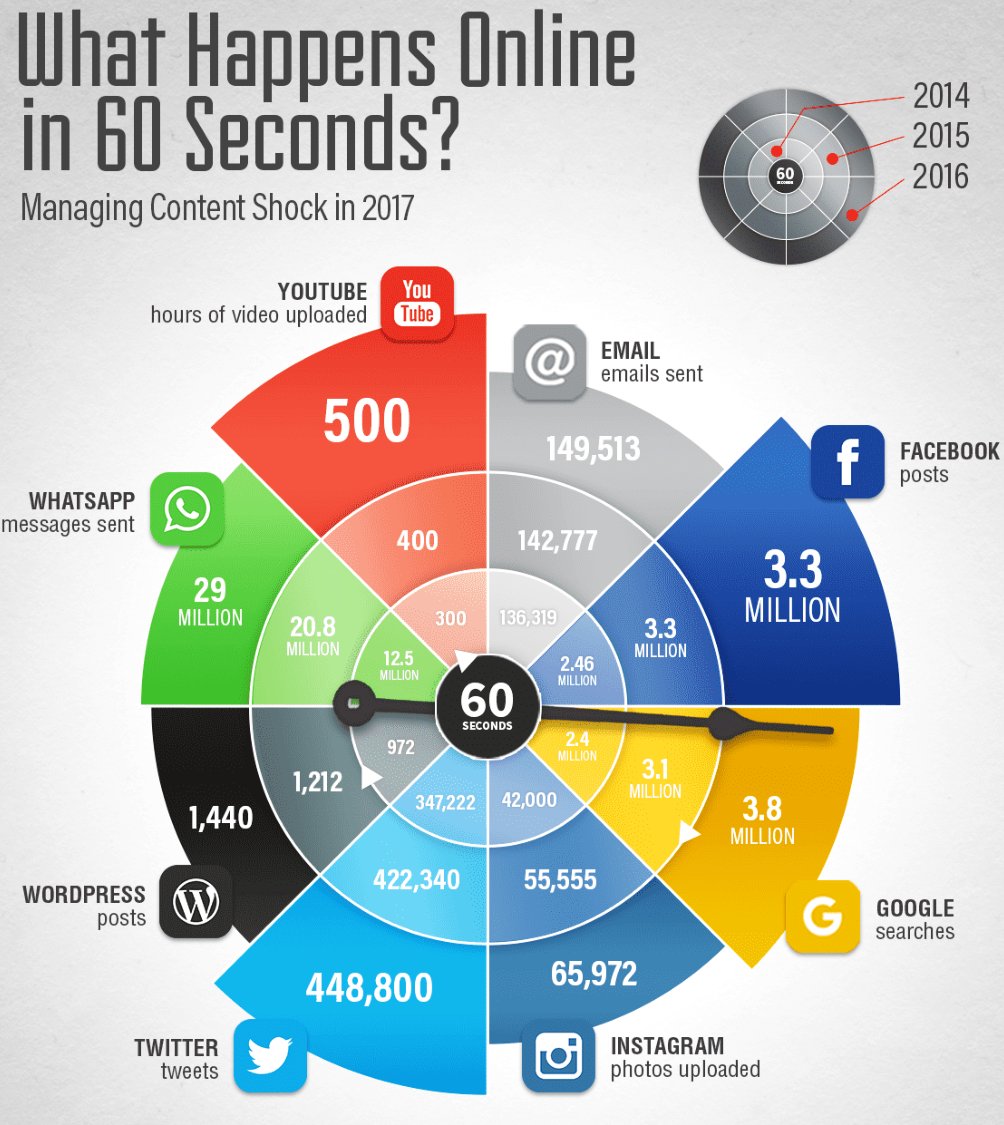
\includegraphics[width=0.95\linewidth]{chapter1/res/media_statistics.pdf}
    \captionof{figure}{大数据时代下图像视频等媒体数据呈现爆炸式增长}
    \label{ch1:fig:media_statistics}
\end{wrapfigure}

视觉是人类感知外界客观世界的主要信息来源,而计算机视觉技术旨在让机器能够像人一样感知物理世界。计算机视觉技术的发展和进步,是众多人机交互技术的基石,也是人类社会迈向真正人工智能时代至关重要的一步。目前,随着互联网技术、社交媒体技术及数字媒体设备的快速发展和普及,图像、动态图、视频等视觉媒体数据已经呈现爆炸式增长。如图~\ref{ch1:fig:media_statistics}所示\footnote{https://www.smartinsights.com/internet-marketing-statistics/happens-online-60-seconds/},截止到2016年,视频分享网站YouTube每分钟上传约500小时视频数据,图像分享社区Instagram每分钟上传约65972张图像数据。面对海量的视觉媒体数据,利用计算机视觉技术对媒体数据进行感知、理解和推理,从而实现对海量视觉媒体数据的快速检索和利用,对便利人们的日常生活、推动社会的进步有着十分重大的意义和应用价值。

另一方面,如图~\ref{ch1:fig:datasets_examples}所示,随着近年来众多大规模人工标注的图像和视频数据集的出现~\cite{lin2014microsoft,russakovsky2015imagenet,krishna2017visual,karpathy2014large,miech2019howto100m}和深度学习技术的突破~\cite{lecun2015deep,krizhevsky2012imagenet},基于深度学习的计算机视觉技术已经取得了长足的进步。例如,在大规模图像分类数据集ImageNet上,Top-1类别的分类准确率高达88.4\%、Top-5类别的分类准确率高达98.7\%~\cite{xie2019self}。然而,现有的计算机视觉技术还远远不能实现大规模的落地应用,这主要原因是由于日常生活中的媒体数据中的视觉场景通常包含大量的物体以及物体间的交互,而对复杂视觉场景的识别和理解本身存在巨大挑战。

\begin{figure}[t]
    \centering
        \includegraphics[width=0.95\linewidth]{chapter1/res/datasets_examples.pdf}
    \caption{众多大规模人工标注的图像和视频数据集推动计算机视觉的发展}
    \label{ch1:fig:datasets_examples}
\end{figure}

具体来说,对复杂视觉场景进行识别和理解,主要包含四个层次:对场景内单个物体的识别(\textbf{物体识别})、对场景内所有物体以及物体间的视觉关系的识别(\textbf{场景识别})、对整个视觉场景内容的理解(\textbf{场景理解})、以及在整个视觉场景理解的基础上进行知识推理(\textbf{场景推理})。本文将针对这四个不同层次的场景理解,逐步地对复杂视觉场景的识别、检测和推理进行研究。如图~\ref{ch1:fig:scene_understanding}所示,本文的关键技术线路主要包括物体分类、场景图生成、视觉描述生成、视觉检索和视觉问答等具体研究任务:

\begin{figure}[t]
    \centering
        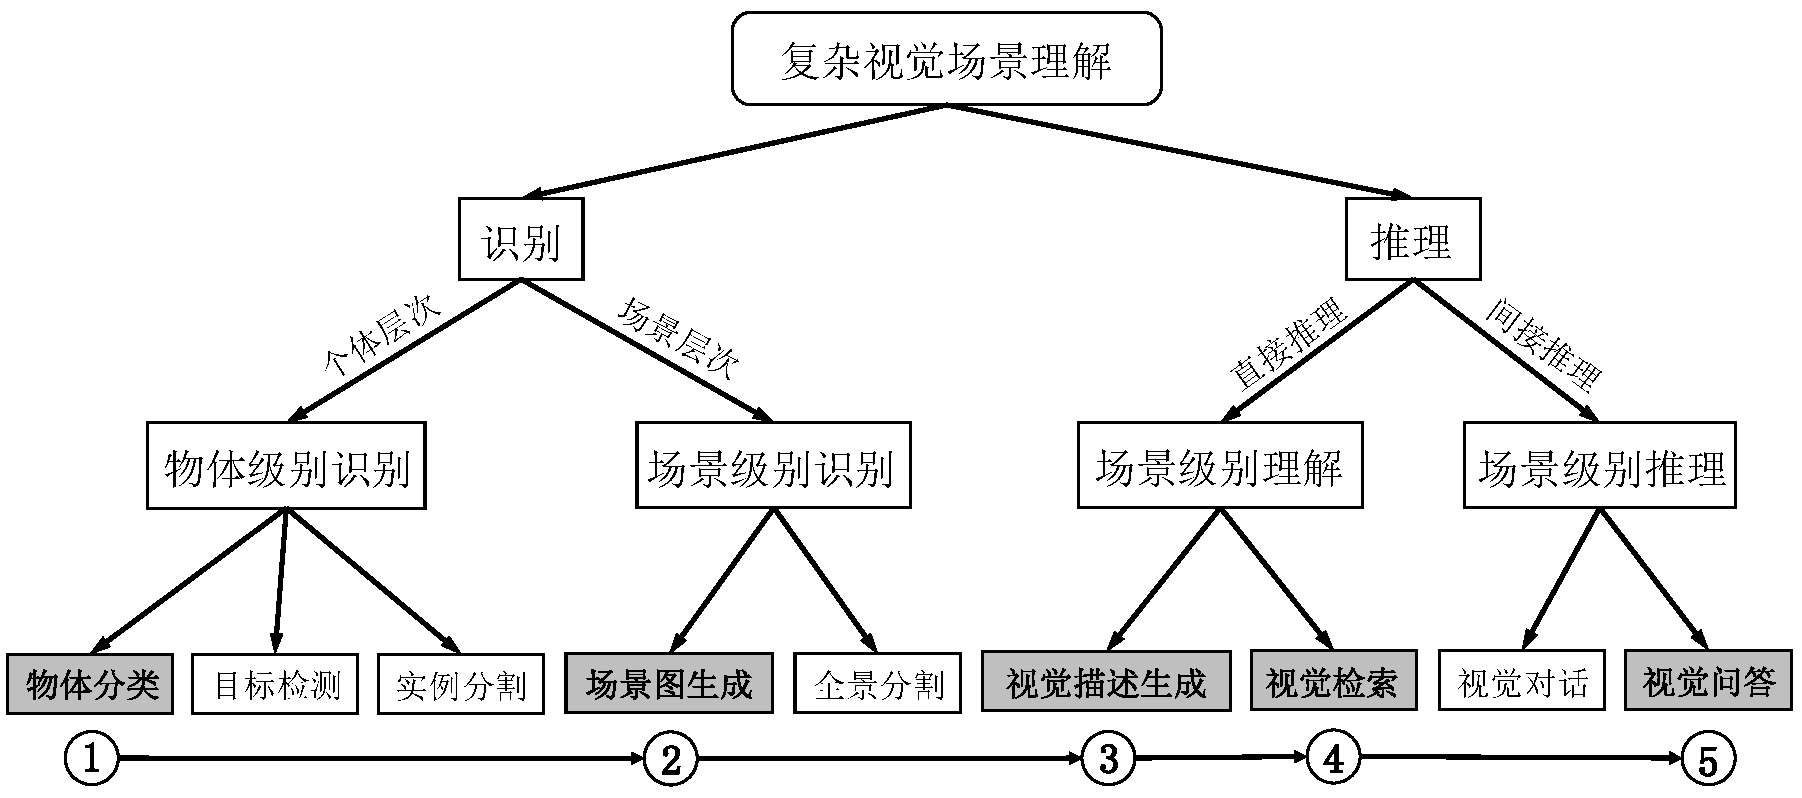
\includegraphics[width=0.95\linewidth]{chapter1/res/scene_understanding.pdf}
    \centering
    \caption{复杂场景识别、检测和推理的关键技术路线}
    \label{ch1:fig:scene_understanding}
\end{figure}

\begin{asparaenum}
\item \textbf{物体识别}:视觉场景理解的首要步骤就是对场景内包含的单个物体进行个体层次的识别。作为计算机视觉领域中一个最基本的问题,个体层次的物体识别结果将直接影响后续对整个视觉场景进行场景层次的识别、理解和推理的结果。根据物体识别的粒度,物体识别通常可以分为物体分类、目标检测、实例分割等具体任务。其中物体分类任务~\cite{russakovsky2015imagenet}的目标是对物体进行多类别分类,而目标检测任务~\cite{ren2015faster,liu2016ssd,redmon2016you}和实例分割任务~\cite{he2017mask}需要在物体分类的基础上,同时对物体的大致边框位置或精确像素位置进行定位。随着卷积神经网络(Convolutional Neural Network, CNN)的发展,在理想实验条件下(即每个类别的训练样本足够充足),物体识别技术已经可以达到较高的准确率。然而,在日常生活中,大量的类别缺乏足够的训练样本。例如,在大规模图像分类数据集ImageNet中,除了最常见的1000类图像以外,在剩余的21814个类别中,有296个类别只有一张训练样本图像~\cite{russakovsky2015imagenet}。为了让物体识别扩展到更加接近实际应用的场景中,基于少样本(Few-Shot Learning, FSL)~\cite{fei2006one}或零样本(Zero-Shot Learning, ZSL)~\cite{lampert2009learning}的物体识别逐渐成为近年来的研究热点。尤其是零样本物体分类问题中,目前的模型普遍存在属性丢失的问题(semantic loss),这大大限制模型的迁移能力。本文主要聚集在零样本物体分类中,研究如何尽可能多地保持物体属性,提升模型在不同测试类别中的迁移能力。

\item \textbf{场景识别}:对整个场景进行理解,除了需要对场景中所有的单个物体进行识别外,还需要对场景中所有物体间的视觉关系(场景图生成~\cite{johnson2015image})和所有不规则物体(全景分割~\cite{kirillov2019panoptic})进行识别。尤其对于复杂场景来说,通常包含大量的视觉关系(visual relationship),而这些视觉关系本身也可以提供丰富的语义间的内在联系,反过来帮助物体的识别。结合所有的物体以及物体间的视觉关系,可以将非结构化的视觉场景转换成结构化的场景图(scene graph)。目前的场景图生成模型都是将所有物体和视觉关系分类的交叉熵之和作为优化目标,忽略了不同物体对整体场景图的不同重要性。本文主要聚焦在场景图生成任务的研究上,研究如何设计更加鲁棒的优化目标函数,提升场景图生成质量。

\item \textbf{场景理解}:在对整个场景中所有的元素(规则物体、不规则物体、视觉关系等)都完成识别之后,就可以开始对场景内容进行理解和推理。就场景理解而言,如何判断模型对视觉场景的理解程度,通常缺乏统一和标准的衡量和评价指标。随着自然语言处理领域的发展,众多视觉和文本融合的多模态任务开始作为场景理解的代理任务:如视觉描述生成~\cite{vinyals2015show}、视觉检索~\cite{gao2017tall}等。视觉描述生产任务需要模型生成自然描述语句来描绘整个视觉场景的内容,通过衡量描述语句的生成质量,来反映模型的理解程度。视觉检索任务需要模型检索与给定查询内容完全一致的视觉场景,通过衡量检索的结果,来反映模型的理解程度。本文将同时聚焦视觉描述生成和视觉检索任务,研究如何设计更加合理的网络结构,帮助对视觉场景的理解。

\item \textbf{场景推理}:对场景进行识别和理解之后,更进一步是希望计算能够像人类一样做场景推理。视觉问答~\cite{antol2015vqa}或视觉对话~\cite{das2017visual}等任务,通常被看作是一种视觉图灵测试~\cite{malinowski2014towards,geman2015visual},用来判断模型的推理能力。由于测试问题的自由和开放性,理论上一个理想的模型需要具备物体识别、场景识别、空间推理、常识推理等多方面的能力。在理论上,通过对这类问题的求解,可以进一步思考和理解人类对外界世界的感知和推理过程;在实际应用上,可以帮助人类更好的与机器完成互动,推动社会的进步。本文将主要聚焦到视觉问答任务的研究上,研究如何突破近年来视觉问答研究的瓶颈(即模型受文本偏置影响较大),帮助提升视觉问答模型的鲁棒性。
\end{asparaenum}

\section{研究内容}

本文主要研究如何对复杂视觉场景进行不同层次的识别和理解,结合目前现有的研究技术,提出更加优化的学习算法和更加合理的网络结构设计,具体可以归纳为图~\ref{ch1:fig:technique_summary}中所示方法。本文使用深度学习的方法对复杂场景理解中上述关键技术进行研究,具体包括以下内容:

\subsection{基于属性保持对抗学习的零样本物体分类}
对视觉场景进行识别和理解,首先我们需要对场景中的单个物体的类别进行识别,其中涉及到的关键技术为零样本物体分类,也称零样本学习。

目前主流的零样本物体分类方法都是基于嵌入映射的框架,这类方法不可避免的存在属性丢失的问题。针对这一普遍问题,本文提出一种全新的零样本学习框架:属性保持的对抗网络学习。该网络通过引入两个独立的映射网络分支,将图像分类和图像重建两个相互冲突的任务分离出来,然后利用对抗网络学习让重建子空间的部分属性迁移到分类子空间中,从而使分类网络的映射向量保持尽可能多的属性,提升模型对不同的新类别的迁移能力。本文提出的零样本物体分类方法不仅可以逼真地重建回原始图像,同时可以大幅度提升零样本分类的准确率。

\begin{figure}[h]
    \centering
        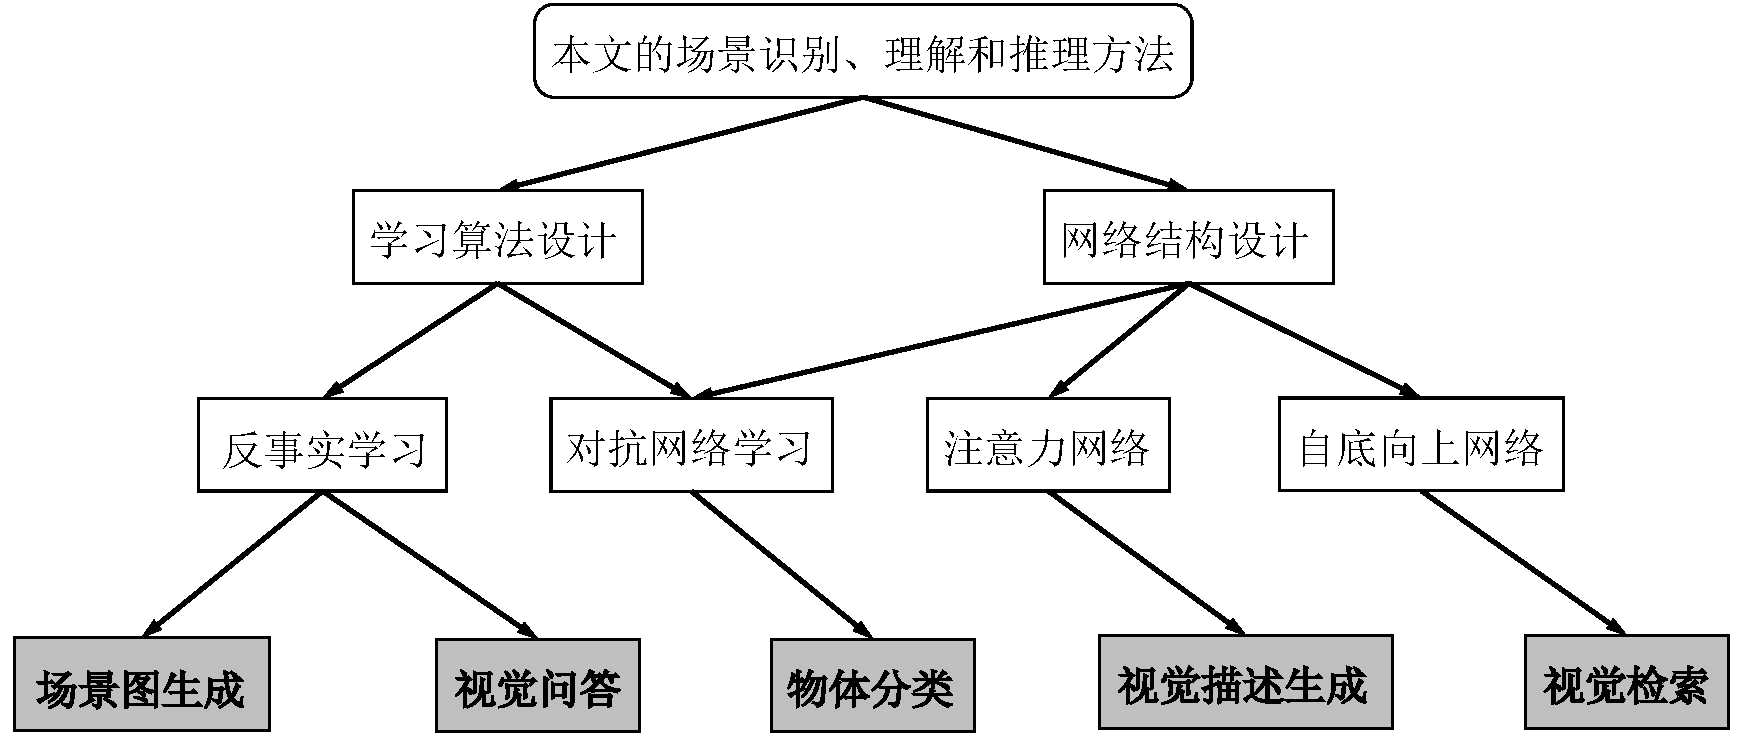
\includegraphics[width=0.95\linewidth]{chapter1/res/technique_summary.pdf}
    \centering
    \caption{复杂场景识别、检测和推理的关键技术研究方法}
    \label{ch1:fig:technique_summary}
\end{figure}


\subsection{基于反事实多智能体学习的场景图生成}
在复杂场景理解中,除了需要对单个的物体进行识别,还需要检测物体间的视觉关系。图像场景图生成任务主要研究如何充分利用场景中所有物体和物体关系之间的内在联系,提升最终所有物体和视觉关系整体的检测结果。

现有的场景图生成方法基本都是将场景内所有的物体和视觉关系分类的交叉熵之和作为模型的优化目标,并将所有的物体和视觉关系的预测认为是相互独立的。这种优化目标忽略了场景中不同物体的重要性,容易使模型陷入局部最优解。本文提出一种全新的框架,将场景图生成问题看成是一种多智能体协同决策问题,其中图像中每个物体为独立的智能体。每个智能体通过预测不同的类别(动作),提升整体的场景图生成质量。同时,本文基于反事实学习,提出一种反事实基准模型,有效地对不同物体的决策分配不同的训练梯度。本文提出的反事实多智能体学习,可以显著提升物体的类别预测,进而提升整个场景图的生成质量。


\subsection{基于多层空间和通道注意力网络的视觉描述生成}

视觉描述语句生成是一种典型的视觉场景理解任务。该任务要求模型对整个视觉场景进行充分的理解,然后生成准确的自然语言描述语句。

现有的图像描述生成模型都是基于编码-解码框架(encoding-deconding framework):即利用卷积神经网络对输入图像进行编码,然后利用递归神经网络(Recurrent Neural Network, RNN)将编码的特征向量解码成自然语句。为了提升描述语句生成的质量,空间注意力机制被广泛的使用在现有的视觉描述生成模型中。这些模型只考虑在空间维度上使用注意力机制,然而,卷积神经网络的特征图(feature map)除空间维度外,还包含通道和层级两个维度。本文,提出一种全新的多层空间和通道注意力网络,充分考虑特征图的三个维度信息,大大提升编码向量的表达能力,使得模型生成更加准确的描述语句。同时,在生成语句的过程中,帮助理解卷积神经网络中特征图的变化过程。

\subsection{基于密集型自底向上框架的视觉检索}

视觉检索任务也是一种常见的视觉场景理解任务。给定一个查询(query),模型首先需要对所有的视觉场景内容进行充分的理解,然后输出与查询内容相匹配的视觉内容。在此关键技术上,我们以视频片段的检索作为切入点,研究基于查询的视频片段检索任务。

本文首先分析了现有基于查询的视频片段检索的主流框架(自顶向下模型和稀疏型自底向上模型)的优缺点,针对目前稀疏型自底向上模型的设计缺陷,我们提出了一种全新的密集型自底向上框架。该框架包含一个密集型头网络,通过将边界预测问题分解成相关性预测和边界回归两个问题,大大降低了模型对视频动作边界定位的难度。同时,我们提出一个基于图卷积的特征金字塔层,来增强骨干网络编码的特征。该框架大大提升了自底向上模型的检索准确率。对于两种不同的查询输入(自然语句和视频片段)任务,本文提出的密集型自底向上模型都达到了目前最先进水平。

\subsection{基于反事实样本生成的视觉问答}

视觉场景理解的最终目标就是能够做到视觉推理。视觉问答是一个典型的视觉推理任务,通过对场景相关的内容进行提问,模型需要充分理解场景中的所有元素以及简单的逻辑推理关系。

本文针对于目前视觉问答模型中的普遍问题:模型受文本偏置影响较大,提出了一种全新的反事实样本生成机制。通过遮盖部分图像或者问句中的重要内容(图像区域或问句单词),同时更改标准答案,合成反事实样本。通过合并原始训练样本和新的反事实样本,迫使模型关注样本中被遮盖的重要内容,让模型在决策时关注正确的视觉区域和单词,提升模型的准确率和鲁棒性。本文提出的反事实样本生成机制可以无缝地运用到任意的视觉问答模型中,帮助提升模型回答准确率。

\section{本文组织结构}
本文通过对复杂视觉场景理解中的识别、检测和推理中的一系列典型问题,提出了多个新的优化算法和网络结构。全文共分为八章,后续章节安排如下:

\begin{asparaitem}

\item 第二章介绍了与本文相关的关键技术研究,就零样本物体分类、图像场景图生成、图像描述语句生成、视频片段检索和视觉问答等几方面的相关工作和本文的关系进行综述。

\item 第三章介绍了基于属性保持的对抗网络学习的零样本物体分类方法。本章首次提出图像分类与图像重建本质上是相互冲突的两个子任务。算法通过利用对抗学习的思想,对图像分类语义特征与图像重建语义特征进行对抗学习,让图像分类语义特征能够像图像重建语义特征保持尽量多的属性,进而提升零样本物体分类的结果。此项工作发表在国际顶级计算机视觉会议CVPR上.

\item 第四章介绍了基于反事实的多智能体学习的图像场景图生成方法。本章首次提出将场景图生成任务转化为多智能体协同决策任务,直接将整个场景图的生成质量当成优化目标,有效地对不同物体的预测类别赋予不同的梯度,显著提升物体类别的预测性能和整体场景图的生成质量。此项工作发表在国际顶级计算机视觉会议ICCV上。


\item 第五章介绍了基于多层空间和通道注意力网络的图像描述语句生成方法。本章首次提出通道注意力机制,通过对图像卷积网络的特征图在通道维度进行加权,让模型能关注到不同通道的语义信息。通过融合空间注意力机制和通道注意力机制,本章提出一种全新的多层空间和通道注意力网络,不仅极大地提升了描述语句的生成质量,也加深了人们对卷积网络特征图的理解。此项工作发表在国际顶级计算机视觉会议CVPR上。


\item 第六章介绍了基于密集型自底向上网络的视频片段检索方法。本章首次提出了一种密集型自底向上网络框架。通过提出全新的密集型头网络,解决了现有稀疏型自底向上网络框架的所有缺点。同时,本章提出一个图特征金字塔层,来增强查询和视频融合后的特征序列。通过结合密集头网络和图特征金字塔层,显著地提升了检索结果。此项工作发表在国际顶级人工智能会议AAAI上。


\item 第七章介绍了基于反事实样本生成的图像视觉问答方法。本章首次提出了一种通用的反事实训练样本生成方法,让视觉问答模型在决策时能够更加关注正确的图像区域或问句单词,提升视觉问答准确率和模型的鲁棒性。提出的样本生成方法可以无缝地运用于多种图像视觉问答模型中,持续地提升回答准确率。此项工作已经投稿至国际顶级计算机视觉大会CVPR上。


\item 第八章对全文介绍的工作进行了总结,并提出了对进一步对复杂场景理解的识别、检测和推理的研究内容以及今后的研究展望。

\end{asparaitem}


\section{本章小结}
本章对复杂视觉场景的识别、检测和推理问题进行了叙述,分别介绍了研究背景、本文的主要研究内容以及全文的组织结构。


\chapter{相关研究综述}

\section{零样本物体识别}

\section{图像场景图检测}

\section{图像描述语句生成}

\section{图像视觉问答}

\section{视频片段检索}
\chapter{基于属性保持的零样本物体分类方法}


零样本物体分类旨在对训练过程中从未见过类别的图像进行分类。为了解决零样本物体分类问题,本章我们提出了一个全新的学习框架:属性保持的对抗网络学习(Semantics-Preserving Adversarial Embedding Networks, SP-AEN)。SP-AEN主要解决了一个目前主流零样本分类框架(基于嵌入映射的模型)中不可避免的问题:语义损失。语义损失是指在训练集的训练过程中,模型往往容易“丢失”一些对训练类别来说区分性不大的属性,但是这些属性可能对测试集(包含不可知的未见类别的图像)非常有用。具体来说,SP-AEN通过引入一个新的映射函数,从而将两个冲突的任务:分类和重建进行分离,映射到两个子空间中。通过对抗学习,SP-AEN可以让重建子空间中部分属性迁移到分类子空间,实现对未见类别的分类。通过与现有零样本分类方法的对比,SP-AEN不仅仅在分类性能上有大幅提升,同时可以生成非常逼真的图像,表现出非常好的属性保持效果。在通用的四个数据集中:CUB、AWA、SUN和aPY, SP-AEN比现有最好的零样本分类方法~\cite{xian2017zero}在H值上分别提升了12.2\%、9.3\%、4.0\%和3.6\%


\section{问题描述}


零样本物体识别(Zero-Shot Recogintion, ZSR)或零样本学习(Zero-Shot Learning, ZSL)是为了能够对训练过程未见过的新类别图像进行分类识别。目前,关于零样本学习问题的难点,学界的共识是如何将已见类别的知识迁移到未见类别上。尽管到目前为止,已经有非常多的零样本分类方法,这些方法都是依据一些非常简单和直观的机制。例如,虽然“浣熊”这个类别在训练的时候没有见过,但是我们仍然可以识别出浣熊的图像,通过检查浣熊这个类别特有的一些属性特征,像“有条纹的尾巴”~\cite{farhadi2009describing,lampert2009learning,zhang2013attribute,li2010object}、“像狐狸的外观”~\cite{torresani2010efficient,li2010object}、以及“浣熊”这个类别的语义信息~\cite{pennington2014glove,mikolov2013distributed}。这些属性特征通常在训练阶段被建模,然后期待在测试阶段中可以在所有的类别(已见类别和未见类别)中共享。经过数十年的发展,目前的零样本学习框架已经从初始基于属性分类器的模型~\cite{lampert2009learning}发展到基于嵌入映射的模型~\cite{akata2015label,frome2013devise,weston2010large}。这种基于嵌入映射的模型往往简单有效,如图~\ref{ch3:fig:zsl_paradigms}(a)所示,这种模型首先将图像从视觉空间(V)映射到语义空间(S),同时,图像类别的语义特征也在该语义空间中。这样映射之后,零样本学习问题就“退化”成一个最近邻的类别查找问题。

\begin{wrapfigure}{r}{0.6\linewidth}
    \centering
        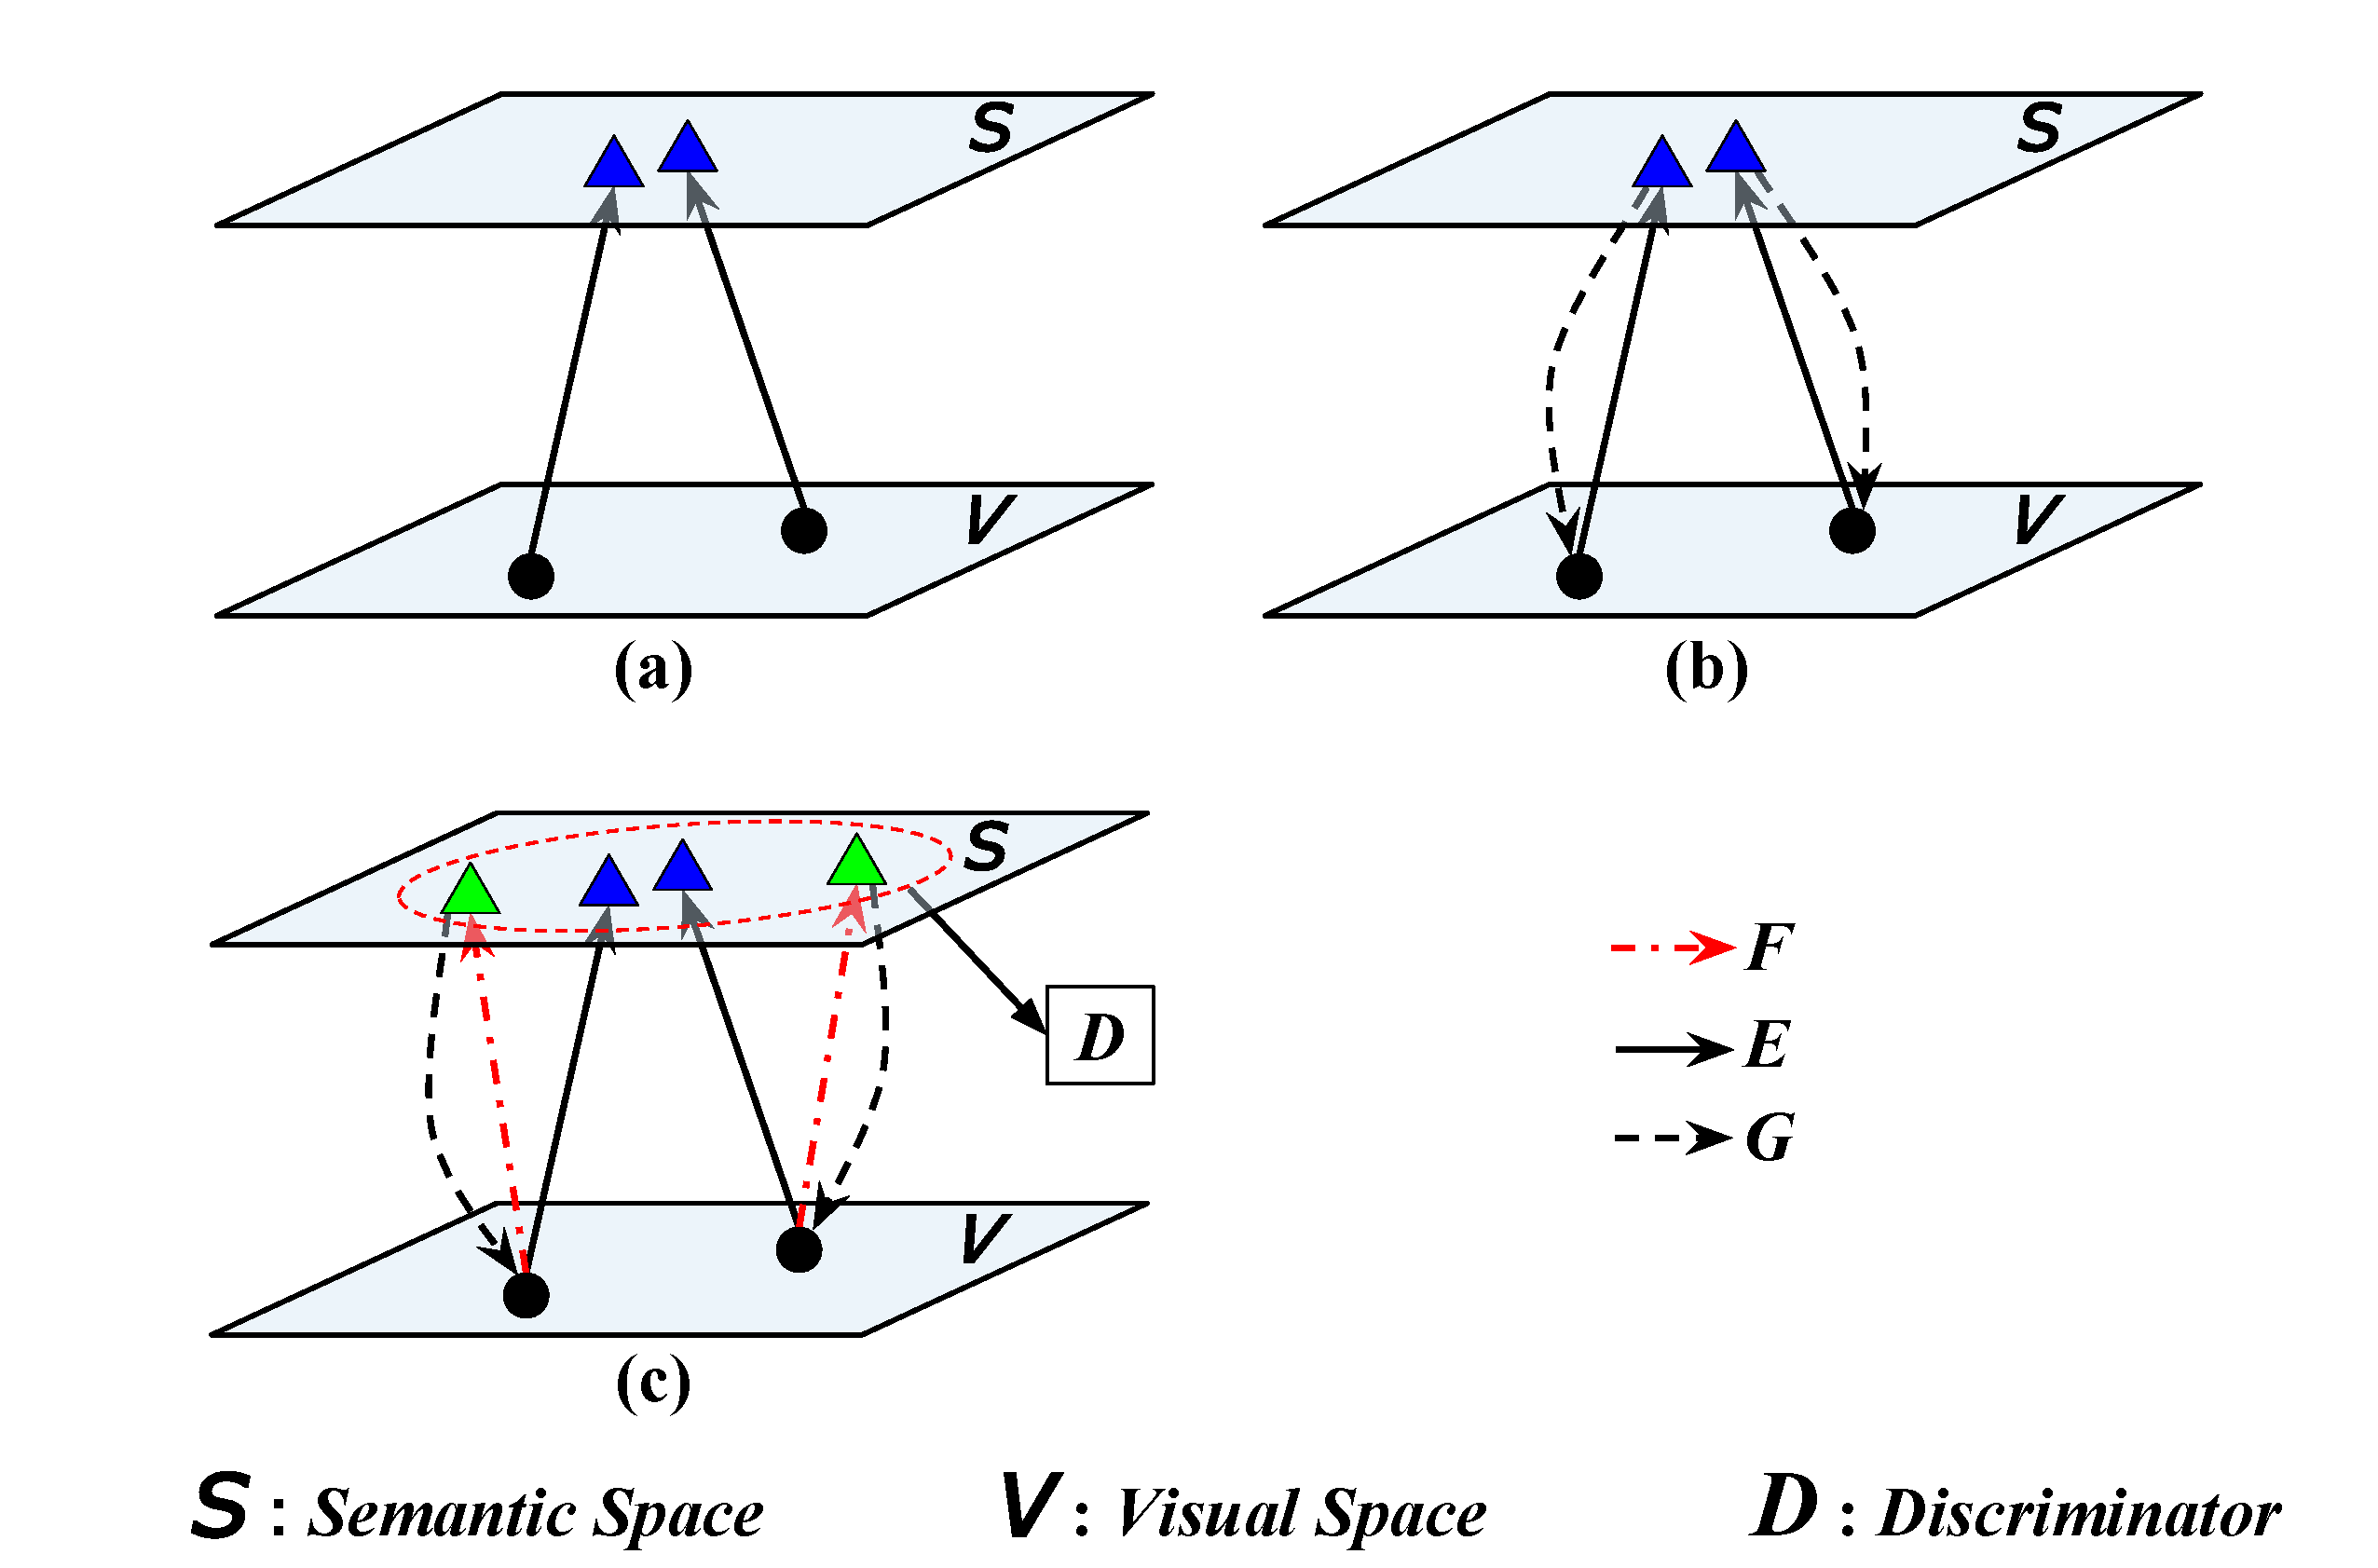
\includegraphics[width=0.95\linewidth]{chapter3/res/zsl_paradigms.pdf}
    \captionof{figure}{三种典型的零样本学习框架}
    \label{ch3:fig:zsl_paradigms}
\end{wrapfigure}

这种嵌入映射模型的知识迁移能力受限于\textbf{语义损失}的问题。如图~\ref{ch3:fig:zsl_paradigms}所示,模型丢失一些对训练集图像方差较小的属性(即,不同类之间区别小的属性)有利于训练集的分类。然而,由于训练集和测试集之间存在差异,这些“丢失”的属性可能对测试集来说具有较大的区别性,这样就会造成对测试集分类的困难。虽然类别在语义空间是一个单独的“点”,具有丰富的语义信息,但是将所有同类的图像从视觉空间映射到这个点附近,就不可避免地造成部分属性的丢失~\cite{lazaridou2015hubness,fu2015transductive}。


为了尽可能多地减少属性的丢失,一个可能的解决方法是通过图像重建,即先将图像从视觉空间映射到语义空间中,然后将语义空间的特征映射回视觉空间。如果映射后的视觉空间的特征能够重建初始的图像,说明语义空间的特征已经尽可能多地保持了原有的属性,否则将无法重建~\cite{kim2017learning,yi2017dualgan,zhu2017unpaired,he2016dual}。然而,图像重建和图像分类是两个相互冲突的目标:前者希望能够尽可能多地保持图像的细节,而后者希望只关注类别差异性大的特征、忽略不相关的特征。例如,只用“头”或者“躯干”就可以充分地对“人”这个类别进行识别分类,而一些其他的颜色属性,如“红色”或者“白色”就需要忽略。为了进一步展示,如图~\ref{ch3:fig:zsl_paradigms}(b)假设 $E$: $\mathcal{V}\rightarrow \mathcal{S}$和$G$: $\mathcal{S}\rightarrow \mathcal{V}$ 是视觉空间与语义空间中的两个映射函数。对于图像分类,我们希望视觉空间中同一类别的两个图像$x, x'\in \mathcal{V}$在语义空间能够接近$s, s'\in\mathcal{S}$, 即, $E(x) = s \approx s' = E(x')$;对于图像重建,我们希望$G(s)\approx x$和$G(s')\approx x'$,这样就很难满足$s\approx s'$。因此,同时训练这两个目标(分类和重建)对于保持属性的效劳往往有限(SAE~\cite{kodirov2017semantic})。如图~\ref{ch3:fig:reconstruction_visualization}所示,如果我们想实现好的分类结果,那往往重建会失败。


\begin{figure}[h]
    \centering
        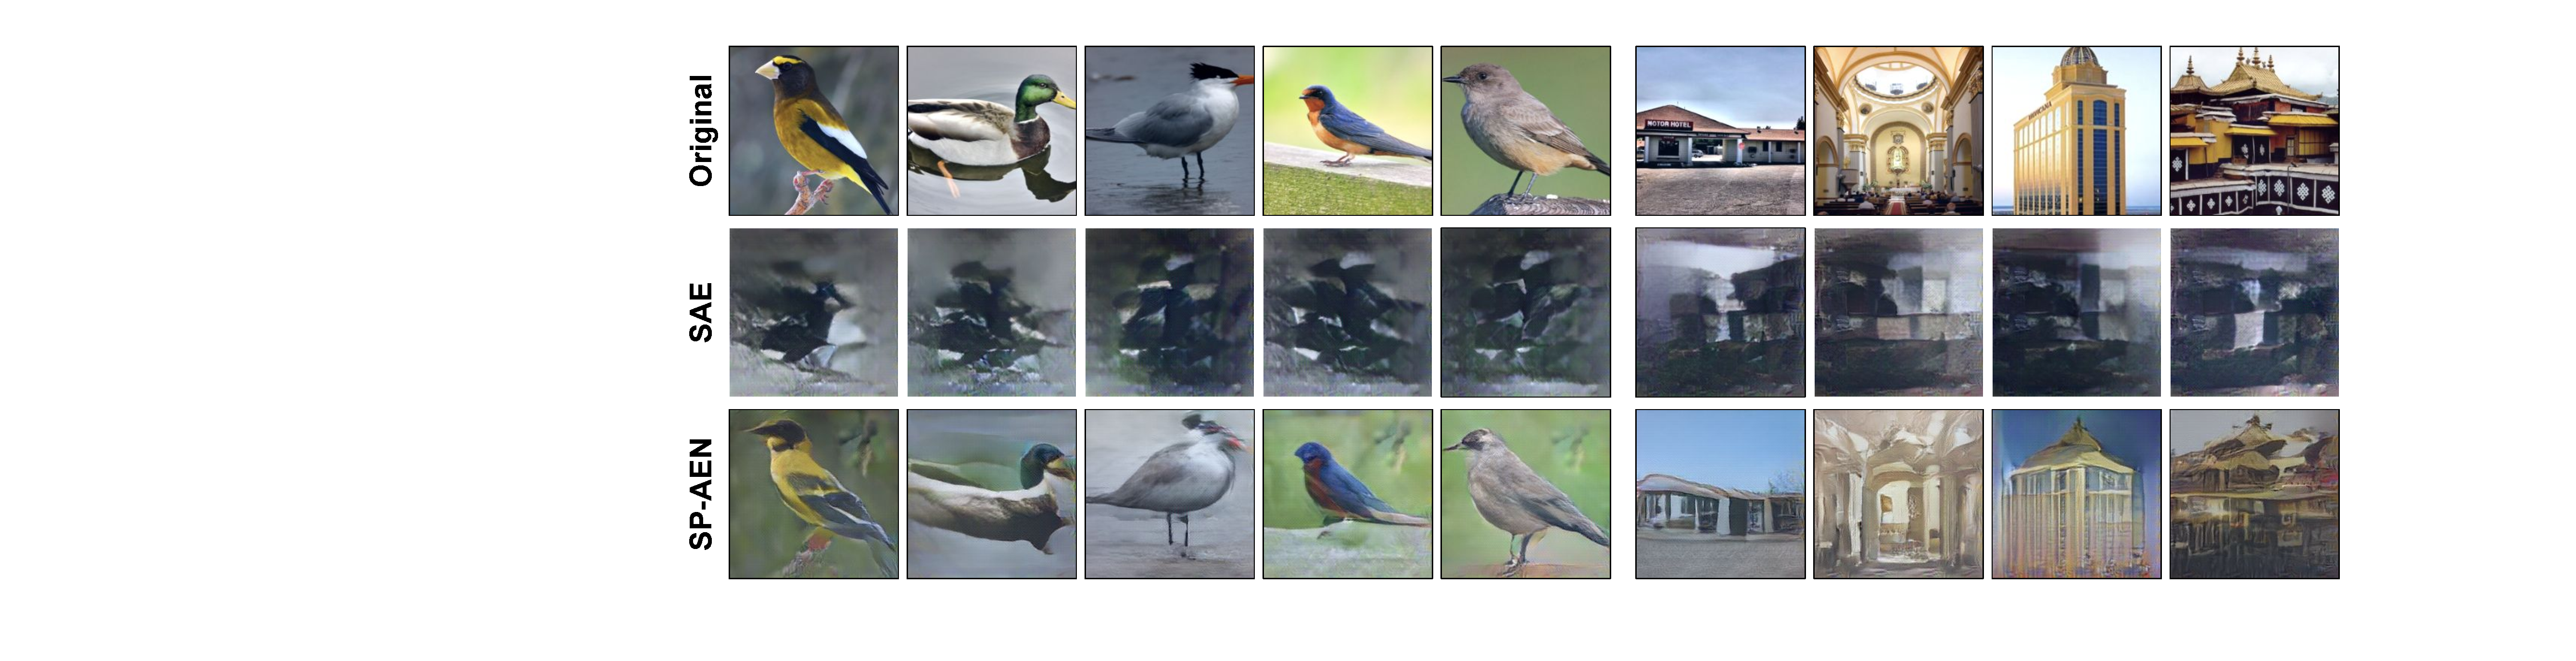
\includegraphics[width=\linewidth]{chapter3/res/reconstruction_visualization.pdf}
    \caption{现有模型SAE~\cite{kodirov2017semantic}和提出模型SP-AEN的图像重建结果对比}
    \label{ch3:fig:reconstruction_visualization}
\end{figure}

为了缓解分类任务和重建任务的冲突,本文提出一个全新的视觉-语义映射的框架:属性保持的对抗网络学习(SP-AEN)。如图~\ref{ch3:fig:zsl_paradigms}(c)所示,我们引入一个新的映射函数$F$: $\mathcal{V}\rightarrow \mathcal{S}$和一个对抗优化目标~\cite{goodfellow2014generative}。映射函数$F$和对抗训练的目的是让判别器$D$无法区分这两个不同的映射分布$E(x)$和$F(x)$。具体来说,这样做有两个好处:(1)\textbf{语义迁移}:虽然对于单独的分类映射函数$E$来说,语义损失是不可避免的。我们通过利用判别器$D$的训练,让分类映射向量$E(x)$和重建映射向量$F(x)$在同一个分布下,实现属性特征的迁移,让$E(x)$尽可能地保持更多的属性。(2)\textbf{分类任务与重建任务分解}:映射网络$F$和$G$实现重建任务,而映射网络$E$实现分类任务。通过将分类任务和重建任务进行分解,之前的严格条件$G(E(x)) \approx x$和$G(E(x')) \approx x'$变成了$G(F(x))\approx x$和$G(F(x'))\approx x'$,同时$F(x)$与$F(x')$在语义空间中也不需要非常接近。如图~\ref{ch3:fig:reconstruction_visualization}所示,我们的映射$G(F(x))$可以重建出较好的输入图像,说明属性特征能够更好地保持。

本文在四个通用的零样本分类数据集中对模型SP-AEN的效果进行验证:CUB~\cite{wah2011caltech},AWA~\cite{lampert2009learning}, SUN~\cite{patterson2012sun},和aPY~\cite{farhadi2009describing}。相比于目前最好的零样本分类方法~\cite{xian2017zero},SP-AEN在评价指标H值(Harmonic Mean Value)上对于上述四个数据集各自提升了12.2\%,9.3\%,4.0\%,和3.6\%。据我们了解,SP-AEN是第一个能够直接重建回原始图像的零样本分类方法。


\section{属性保持的对抗网络学习}

在本节,我们首先介绍零样本分类任务,然后再具体介绍本章提出模型SP-AEN的各个优化目标的细节。

\subsection{零样本分类预备知识}
给定一个训练集$\{x_i, l_i\}$,其中$x_i\in\mathcal{V}$是图像在视觉空间的映射向量,$l_i\in \mathcal{L}_s$是已见类别的类别标签,零样本分类任务的目标是学习一个分类器。这个分类器不仅可以预测已见类别的图像($\mathcal{L}_s$),也可以预测未见类别的图像($\mathcal{L}_u$)。按照之前工作的总结~\cite{xian2017zero,lei2015predicting},几乎所有先进的零样本分类方法都是基于嵌入映射的。这类方法旨在找到一个映射函数$\mathcal{V}\rightarrow \mathcal{S}$,其中所有的类别标签在语义空间$\mathcal{S}$都是编码成$\mathbf{y}_l\in\mathbb{R}^d$。因此,预测类别标签$l^*$时,可以直接通过简单的最近邻查找:
\begin{equation}\label{ch3:eq:eq_1}
l^* = \max_{l\in\mathcal{L}}~\mathbf{y}^T_l E(x)
\end{equation}
特别地,如果$l\in\mathcal{L}_u$,这是\textbf{传统型零样本分类};如果$l \in\mathcal{L}_s\cup \mathcal{L}_u$,这是\textbf{通用型零样本分类问题}。另外,公式~\eqref{ch3:eq:eq_1}中$E$不一定是线性函数,同样可以利用深度神经网络等非线性函数。


\begin{figure}[tbp]
    \centering
        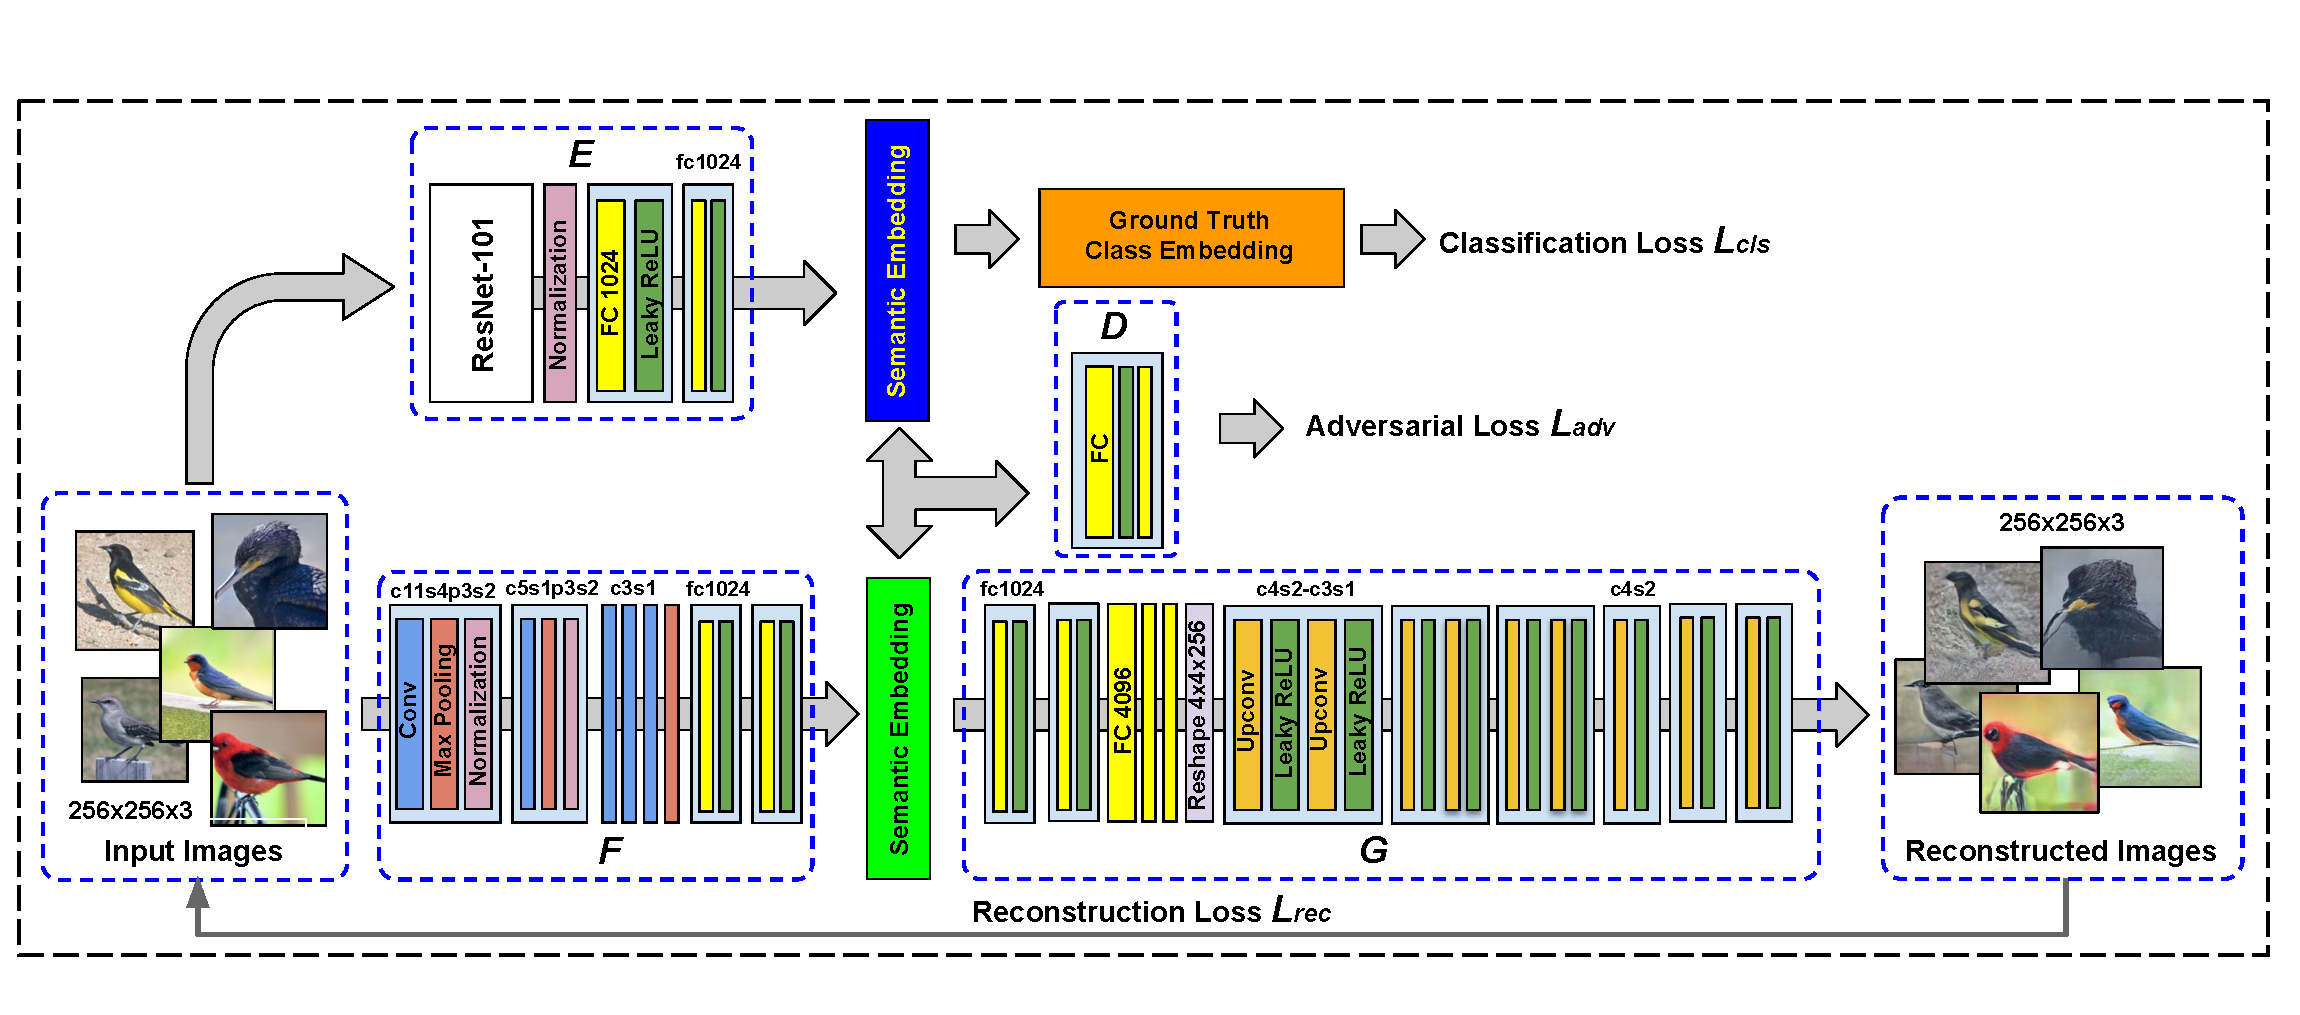
\includegraphics[width=\linewidth]{chapter3/res/sp_aen.pdf}
    \caption{模型SP-AEN的整体结构流程图}
    \label{ch3:fig:sp_aen}
\end{figure}


\subsection{分类任务优化目标}
由于公式~\eqref{ch3:eq:eq_1}的标签预测本质上是一个排序问题,我们使用排序损失(Ranking Loss)作为分类任务的优化目标~\cite{frome2013devise,weston2010large},即给定一个训练样本$(x, l)$,我们希望$\mathbf{y}_l$和$E(x)$之间有一个较大的点积相似度,而负样本$(x,l')$有较小的点积相似度,并且正样本的相似度相比负样本的相似度要大于一定的阈值:
\begin{equation}\label{ch3:eq:eq_2}
L_{cls} = \sum\limits_{l\neq l'}~\max\{0, \gamma - \mathbf{y}_l^T E(x) + \mathbf{y}^T_{l'} E(x)\}
\end{equation}
其中,$\gamma >0$是一个超参数(即阈值)。在每次训练迭代过程中,$l'$是从所有错误的标签中任选一个。

分类任务优化目标$L_{cls}$的目的是让所有的同一类图像的语义空间映射向量$E(x)$都接近与其类别标签$\mathbf{y}$在语义空间的映射向量。它造成的语义损失问题将由后续介绍的两个额外的优化目标来解决。


\subsection{重建任务优化目标}
重建任务的目标是学习一个从语义空间到视觉空间的映射函数$G$: $\mathcal{S}\rightarrow \mathcal{V}$,使得将语义映射向量$s\in\mathcal{S}$可以重建输入图像,并且使差别$\|G(s)-x\|$很小。由于在自编码器中重建任务$s = E(x)$与分类任务是相互冲突的,我们引入一个新的视觉空间到语义空间的映射函数$F$,使得$s = F(x)$。另外,不同于SAE~\cite{kodirov2017semantic}利用卷积神经网络~\cite{he2016deep,simonyan2015very}的输入作为视觉空间$\mathcal{V}$的特征,我们直接利用原始的$256\times 256 \times 3$大小的RGB色彩空间来进行图像重建。这样做的主要原因是,卷积神经网络的输出特征在网络的预训练阶段已经存在语义损失问题。


为了最小化重建损失,映射向量$F(x)$会尽可能地保持多的属性,以便于重建回输入图像。我们参考最新的图像生成工作~\cite{johnson2016perceptual,dosovitskiy2016generating,ledig2017photo},将优化目标定义为:
\begin{equation}\label{ch3:eq:eq_3}
L_{rec} = L_{feat}+\lambda_p L_{pixel}
\end{equation}
其中$L_{feat} = \|\phi\left(G\left(F(x)\right)\right)-\phi(x)\|^2_2$是特征维度上的重建损失函数,帮助图像能够保持细节感知上的相似度。我们使用卷积神经网络AlexNet~\cite{krizhevsky2012imagenet}中$conv5$层来表示$\phi$。$L_{pixel} = \|G(F(x))-x\|^2_2$是像素维度上的重建损失函数,有利于算法的稳定性。


\subsection{对抗学习优化目标}
到目前为止,语义向量$E(x)$和$F(x)$之间没有知识迁移。我们的目标是让$E(x)$从$F(x)$中迁移部分丢失的属性特征。然后,手工直接定义$E(x)$与$F(x)$之间的迁移比较困难。因此,我们借助于对抗学习的思想,来鼓励$E(x)$的分布向$F(x)$的分布靠近,通过“欺骗”判别网络$D$,使$F(x)$的知识向$E(x)$迁移:
\begin{equation}\label{ch3:eq:eq_4}
L_{adv} = \mathbb{E}_{x}\left( \log D(F(x)) \right) + \mathbb{E}_{x'}\left( \log \left[1-D(E(x'))\right] \right)
\end{equation}
其中网络$E$为了减少优化目标$L_{adv}$,而网络$D$希望增大优化目标$L_{adv}$,即:$E^* = \arg\min_E \max_D L_{adv}$。

目前,许多研究工作都发现目标函数$L_{adv}$进行优化容易陷入“塌陷问题”~\cite{arjovsky2017wasserstein}。在我们这个任务中,如果两个同类别的图像$x$和$x'$非常相似,容易导致$\|F(x)-E(x')\|\approx 0$,引起塌陷问题。为了避免塌陷问题,我们参考WGAN的策略~\cite{arjovsky2017wasserstein},极大地增加了模型训练的稳定性。


\subsection{总体优化目标}
将之前提到的分类任务优化目标、重建任务优化目标、以及对抗学习优化目标合在一起,得到最终整体的优化目标:
\begin{equation}\label{ch3:eq:eq_5}
\begin{split}
L (E, F, G, D) = L_{cls}(E) &+ \alpha L_{rec} (E, F, G) \\
&+ \beta L_{adv}(E, F, G, D)
\end{split}
\end{equation}
其中,$\alpha$和$\beta$是参数用于权衡不同的训练目标。最终的目标是得到:
\begin{equation}\label{ch3:eq:eq_6}
E^* = \arg\min\limits_{E, F, G}\max\limits_{D} L(E, F, G, D)
\end{equation}

如图~\ref{ch3:fig:sp_aen}所示,网络$F$是编码网络,网络$G$是解码网络,重建映射向量$F(x)$可以看成是瓶颈层,来约束分类映射向量$E(x)$。另外,SP-AEN可以转换成其他条件下的零样本分类问题,例如半监督条件下,我们只需要给$F(x)$增加一个额外的对抗学习优化目标来近似先验的映射空间。



\section{实验设置与性能分析}
\subsection{零样本物体分类数据集}
\textbf{CUB}~\cite{wah2011caltech}:全称是Caltech-UCSD-Birds 200-2011数据集。它是一个细粒度鸟类别分类数据集,总共包含11788张来自200个细粒度类别的鸟图像,并且每张图像有312个语义属性标注。其中训练集包含150个已见类别的7057张图像,测试集包含150个已见类别的1764张图像和50个未见类别的2967张图像。

\textbf{SUN}~\cite{patterson2012sun}:全称是SUN attribute数据集。它是一个细粒度场景分类数据集,总共包含14340张来自717个场景类别的场景图像,并且每张图像有102个语义属性标注。其中训练集包含645个已见类别的10320张图像,测试集包含645个已见类别的2580张图像和72个未见类别的1440张图像。

\textbf{AWA}~\cite{lampert2009learning}:全称是Animals with Attributes数据集。它是一个动物类别分类数据集,总共包含30475张来自50个类别的动物图像,并且每张图像有85个语义属性标注。其中训练集包含40个已见类别的23527张图像,测试集包含40个已见类别的5882张图像和10个未见类别的7913张图像。由于原始AWA数据集图像版权的问题,我们这里的AWA数据集实际上使用的是AWA2~\cite{xian2017zero}.

\textbf{aPY}~\cite{farhadi2009describing}:全称是Attribute Pascal and Yahoo数据集。它是一个通用的物体分类数据集,总共包含12051张来自32个类别,并且每张图像有64个语义属性标注。其中训练集包含20个已见类别5932张图像,测试集包含20个已见类别1483张图像和12个未见类别的7924张图像。

为了公平地和其他模型进行比较,我们使用Xian等人~\cite{xian2017zero}提供的类别嵌入映射向量,其中每个嵌入映射向量都经过$l_2$范数进行归一化。


\subsection{实验设定与零样本物体分类评价指标}
\noindent{\kaishu{实验设定}}:
为了评估模型对零样本物体分类的结果,我们采用三种实验设定:
\begin{asparaenum}
\item U$\to$U: 测试图像的类别和可以预测的类别都只是未见类别;

\item S$\to$T: 测试图像的类别是未见类别,但是可以预测的类别是未见类别和已见类别的总和;

\item U$\to$T: 测试图像的类别和可以预测的类别都是未见类别和已见类别的总和。
\end{asparaenum}
通常,U$\to$U被称为传统型零样本分类,而U$\to$T被称为通用型零样本分类。

\noindent{\kaishu{评价指标}}:
我们参考现有的文献~\cite{xian2017zero},常用的每类平均准确率作为评价指标。对于通用型零样本分类,我们另外使用常用的$H$作为主要的评价指标,其中$H$是已见类别$L_s$的准确率($Acc_{S\rightarrow T}$)和未见类别$L_u$的准确率($Acc_{U\rightarrow T}$)的调和平均数:
\begin{equation} \label{ch3:eq:eq_7}
H = 2\times Acc_{S\rightarrow T}\times Acc_{U\rightarrow T} /(Acc_{S\rightarrow T}+Acc_{U\rightarrow T})
\end{equation}

\subsection{网络模型与参数设置}
\noindent{\kaishu{网络结构}}:整个网络结构都是端到端地直接进行训练。其中映射网络$E$是基于ResNet-101~\cite{he2016deep},输入图像的大小是$224\times224\times3$。映射网络$F$是基于AlexNet~\cite{krizhevsky2012imagenet},然后附加上两层额外的全连接层。重建网络$G$采用类似于生成器~\cite{dosovitskiy2016generating}的结构,通过五个连续的反卷积和非线性操作(leaky ReLU)将向量特征转换成三维卷积特征。


\noindent{\kaishu{参数设置}}:对于本章所有的实验,训练图像都将短边放缩到256个像素。参照AlexNet~\cite{krizhevsky2012imagenet},我们采用了增大十倍训练图像的数据增强方式。为了提升训练速度,映射网络$E$中ResNet-101部分参数始终保持固定,映射网络$F$的参数初始化采用预训练好的AlexNet的参数,重建网络$G$的参数初始化用预训练好的生成器~\cite{dosovitskiy2016generating}。剩余的所有参数都是用MSRA的随机初始化~\cite{he2015delving}。初始的学习率设置为$1e^{-4}$,然后当loss不下降时,学习率降低10倍。


\subsection{零样本物体分类的性能对比}
本节将本章方法与目前最先进的零样本物体分类方法进行对比。这些方法主要可以分类:(1)基于嵌入映射的模型:DeViSE~\cite{frome2013devise}、ALE~\cite{akata2015label}、SJE~\cite{akata2015evaluation}、ESZSL~\cite{romera2015embarrassingly}、LTM\cite{xian2016latent}、CMT/CMT$^*$~\cite{socher2013zero}和SAE~\cite{kodirov2017semantic}。这类方法和SP-AEN一样,将图像从视觉空间映射到语义空间。据我们了解,SAE是现有的唯一一个利用信号重建来解决语义损失的模型。(2)基于属性的模型:DAP~\cite{lampert2009learning}、IAP~\cite{lampert2009learning}、SSE~\cite{zhang2015zero}、CSE~\cite{norouzi2014zero}和SYNC~\cite{changpinyo2016synthesized}。这类方法只适用于有属性标注的情况。

%%%%%%%%%%%%%%%%%%%%%%%%%% SOTA %%%%%%%%%%%%%%%%%%%%
\begin{table}[htbp]
\centering
\scalebox{0.7}{
\begin{tabular}{|c | c | c c c c c c c c c c c c c|}
\hline
Dataset &  & DAP & IAP & SSE & CSE & SYNC & CMT & LTM & DeViSE & ALE & SJE & ESZSL & SAE & SP-AEN \\
\hline
\multirow{4}{*}{SUN} & $Acc_{U\to U}$ & 39.9 & 19.4 & 51.5 & 38.8 & 56.3 & 39.9 & 55.3 & 56.5 & 58.1 & 53.7 & 54.5 & 40.3 & \textbf{59.2} \\
& $Acc_{U\to T}$ & 4.2 & 1.0 & 2.1 & 6.8 & 7.9 & 8.1 & 14.7 & 16.9 & 21.8 & 14.7 & 11.0 & 8.8 & \textbf{24.9} \\
& $Acc_{S\to T}$ & 25.1 & 37.8 & 36.4 & \textbf{39.9} & 43.3 & 21.8  & 28.8 & 27.4 & 33.1 & 30.5 & 27.9 & 18.0 & 38.6 \\
& H & 7.2 & 1.8 & 4.0 & 11.6 & 13.4 & 11.8 & 19.5 & 20.9 & 26.3 & 19.8 & 15.8 & 11.8 & \textbf{30.3} \\
\hline
\multirow{4}{*}{CUB} & $Acc_{U\to U}$ & 40.0 & 24.0 & 43.9 & 34.3 & \textbf{55.6} & 34.6 & 49.3 & 52.0 & 54.9 & 53.9 & 53.9 & 33.3 & 55.4 \\
& $Acc_{U\to T}$ & 1.7 & 0.2 & 8.5 & 1.6 & 11.5 & 7.2 & 15.2 & 23.8 & 23.7 & 23.5 & 12.6 & 7.8 & \textbf{34.7} \\
& $Acc_{S\to T}$ & 67.9 & \textbf{72.8} & 46.9 & 72.2 & 70.9 & 49.8 & 57.3 & 53.0 & 62.8 & 59.2 & 63.8 & 54.0 & 70.6 \\
& H & 3.3 & 0.4 & 14.4 & 3.1 & 19.8 & 12.6 & 24.0 & 32.8 & 34.4 & 33.6 & 21.0 & 13.6 & \textbf{46.6} \\
\hline
\multirow{4}{*}{AWA} & $Acc_{U\to U}$ & 46.1 & 35.9 & 61.0 & 44.5 & 46.6 & 37.9 & 55.8 & 59.7 & \textbf{62.5} & 61.9 & 58.6 & 54.1 & 58.5 \\
& $Acc_{U\to T}$ & 0.0 & 0.9 & 8.1 & 0.5 & 10.0 & 0.5 & 11.5 & 17.1 & 14.0 & 8.0 & 5.9 & 1.1 & \textbf{23.3} \\
& $Acc_{S\to T}$ & 84.7 & 87.6 & 82.5 & 90.6 & 90.5 & 90.0 & 77.3 & 74.7 & 81.8 & 73.9 & 77.8 & 82.2 & \textbf{90.9} \\
& H & 0.0 & 1.8 & 14.8 & 1.0 & 18.0 & 1.0 & 20.0 & 27.8 & 23.9 & 14.4 & 11.0 & 2.2 & \textbf{37.1} \\
\hline
\multirow{4}{*}{aPY} & $Acc_{U\to U}$ & 33.8 & 36.6 & 34.0 & 26.9 & 23.9 & 28.0 & 35.2 & \textbf{39.8} & 39.7 & 32.9 & 38.3 & 8.3 & 24.1 \\
& $Acc_{U\to T}$ & 4.8 & 5.7 & 0.2 & 0.0 & 7.4 & 1.4 & 0.1 & 4.9 & 4.6 & 3.7 & 2.4 & 0.4 & \textbf{13.7} \\
& $Acc_{S\to T}$ & 78.3 & 65.6 & 78.9 & \textbf{91.2} & 66.3 & 85.2 & 73.0 & 76.9 & 73.7 & 55.7 & 70.1 & 80.9 & 63.4 \\
& H & 9.0 & 10.4 & 0.4 & 0.0 & 13.3 & 2.8 & 0.2 & 9.2 & 8.7 & 6.9 & 4.6 & 0.9 & \textbf{22.6} \\
\hline
\end{tabular}
}
\caption{不同零样本物体分类方法在4个数据集上的性能对比}
\label{ch3:tab:sota}
\end{table}
%%%%%%%%%%%%%%%%%%%%%%%%%%%%%%%%%%%%%%%%%%%%%%%%%%%%%

\textbf{定量性能对比}:表~\ref{ch3:tab:sota}总结了不同的零样本分类方法在四个数据集(SUN、CUB、AWA、aPY)和三种不同实验设定下(U$\to$U、U$\to$T、S$\to$T)的性能对比。从表~\ref{ch3:tab:sota}我们能有两个发现:(1)SP-AEN在通用型零样本分类问题能够显著提升性能,如:在$Acc_{U\to T}$和H值两个指标下,SP-AEN能比目前最好的模型提升4\%到12\%。当数据集中训练集和测试集所有属性方差的余弦相似度越大时\footnote{数据集SUN、CUB、AWA、aPY中,训练集和测试集所有属性方差的余弦相似度分别为0.9851、0.9575、0.7459、0.5847。},提升更加明显,这也表明SP-AEN可以有效地缓解语义损失问题。(2)在传统型零样本分类的设定下(U$\to$U),在绝大多数的情况下,SP-AEN可以得到最佳的性能。在U$\to$U设定下,图像类别的搜索空间仅限于未见类别,然而,语义损失问题可能导致未见类别的图像与已见类别非常接近,造成一定的预测错误。

\subsection{零样本物体分类方法分析}

\begin{wrapfigure}{r}{0.55\linewidth}
    \centering
        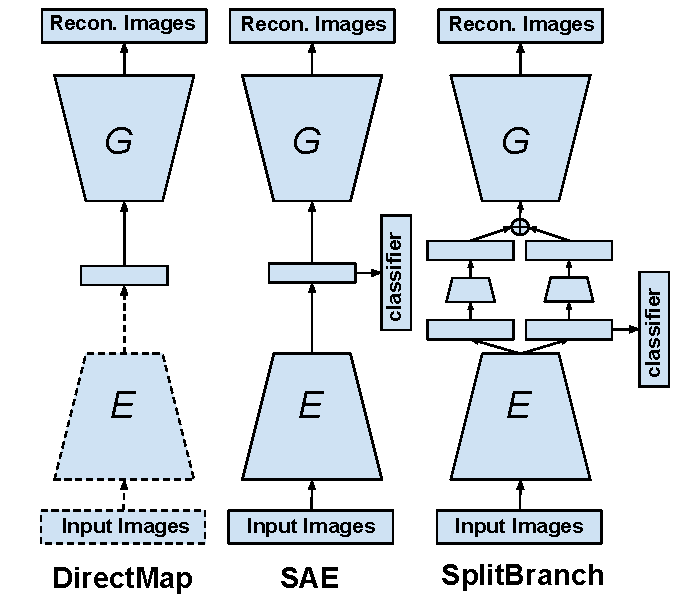
\includegraphics[width=0.95\linewidth]{chapter3/res/conflict.pdf}
    \captionof{figure}{三种图像重建网络框架}
    \label{ch3:fig:conflict}
\end{wrapfigure}

\textbf{分类任务与重建任务的冲突}:为了验证本章提出模型SP-AEN的设计动机:分类任务和重建任务时相互冲突的。如图~\ref{ch3:fig:conflict}所示,我们设计了三种可能的重建网络框架,可以实现SP-AEN中语义空间到视觉空间的重建:(1)\textbf{DirectMap}:对于输入图像,我们使用网络$E$将图像从视觉空间映射到语义空间,得到语义嵌入向量,然后使用网络$G$将语义嵌入向量映射回视觉空间。在该网络中,我们固定$E$的参数,只训练网络$G$的参数。DirectMap可以衡量初始的语义嵌入向量包含多少语义信息。(2)\textbf{SAE}~\cite{kodirov2017semantic}:我们采用与SAE模型相同的框架,用重建网络$G$作为解码网络,分类网络$E$作为编码网络,其中的瓶颈层用来分类任务。在训练阶段,我们同时训练网络$E$和$G$的参数。(3)\textbf{SplitBranch}:我们将网络$E$的输出分别输入到两个不同的支路中,其中一条支路用来分类。然后两条主路再连接到一起,合并的语义特征输入到网络$G$中进行重建。


\begin{table}[htbp]
\centering
\begin{tabular}{|c c| c| c| c|}
\hline
Method & \textbf{SUN} & \textbf{CUB} & \textbf{AWA} & \textbf{aPY} \\
\hline
 DirectMap & 0.079 & 0.069 & 0.075 & 0.085 \\
 SAE & 0.285 & 0.281 & 0.259 &  0.275\\
SplitBranch & 0.070 & 0.058  & 0.059 & 0.076 \\
SP-AEN & \textbf{0.053}  & \textbf{0.040}& \textbf{0.047} & \textbf{0.055} \\
\hline
\end{tabular}
\caption{不同重建网络下重建图像与输入图像之间的平均像素差平方}
\label{ch3:tab:conflict_quantitative}
\end{table}


\begin{figure}[htbp]
    \centering
    \scalebox{0.9}{
        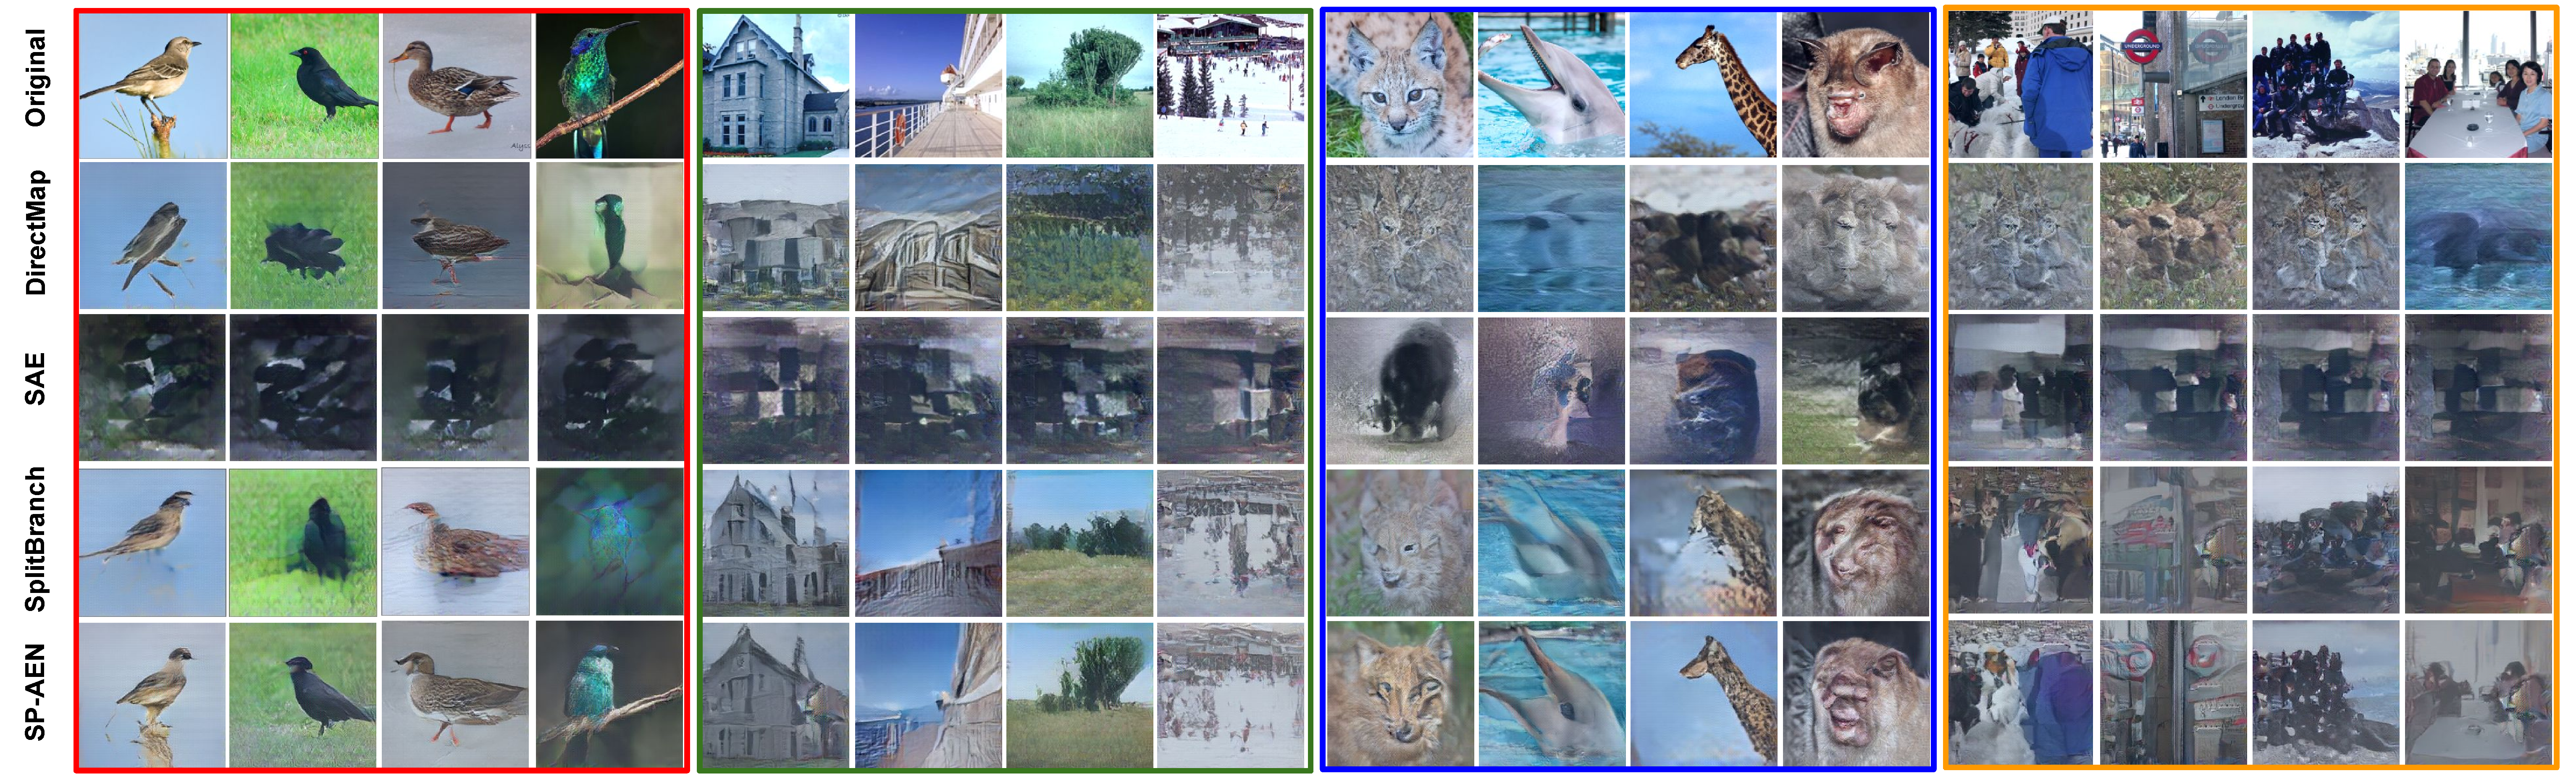
\includegraphics[width=\linewidth]{chapter3/res/conflict_visualization.pdf}    
    }
    \caption{不同图像重建网络框架在数据集CUB、SUN、AWA、aPY上的重建结果}
    \label{ch3:fig:conflict_visualization}
\end{figure}

图~\ref{ch3:fig:conflict_visualization}和表~\ref{ch3:tab:conflict_quantitative}分别表示四个数据集中测试集未见类别图像的重建图像和重建差异。从实验结果中,我们可以有以下结论:(1)在数据集CUB和SUN中,DirectMap重建的图像和SP-AEN非常接近,都具有较好的重建结果。然而,在数据集AWA和aPY中,DirectMap的重建效果有明显下降。同样地,这是由于在数据集CUB和SUN中,训练集和测试集所有属性方差的余弦相似度大于AWA和aPY。(2)如果像SAE模型一样同时训练分类网络E和重建网络G,所有的样本都重建失败。如果像SplitBranch模型一样同时训练,我们可以看到重建效果得到显著的提升,十分接近SP-AEN。但是,我们发现在SplitBranch中,分类分支合并时的权重几乎为零。这一方面说明分类的映射向量基本对重建任务没有贡献,另一方面也引导我们借助对抗学习来实现语义迁移和高质量图像的重建。

\textbf{网络D和网络G的作用}:由于可见类别标签的分数常常大于未见类别标签的分数,通常使用“校准规则”来解决这个问题。具体来说,就是对已见类别的分数减掉一个偏置,然后再和未见类别一起进行排序比较:

\begin{equation}\label{ch3:eq:eq_8}
    l^* = \max_{l\in \mathcal{L}_u \cup \mathcal{L}_s }~\mathbf{y}^T_l E(x) - \gamma \mathbf{1} \left[ l \in \mathcal{L}_s \right]
\end{equation}
其中,指示函数$\mathbf{1} \left[ \cdot \right]$用于判断$l$是否时已见类别,$\gamma \in \mathbb{R}$是校准系数。这个校准规则能够有效地实现对已见类别和未见类别预测之间的权衡。通过改变校准系数$\gamma$,我们可以得到一系列分类准确率($Acc_{U \to T}$和$Acc_{S \to T}$),并且可以画出已见-未见准确率曲线(Seen-Unseen accuracy Curve, SUC)。已见-未见准确率曲线下区域面积(Area Under Seen-Unseen accuracy Curve, AUSUC)也是通用型零样本分类问题中一个常用评价指标,用来评估$Acc_{U \to T}$和$Acc_{S \to T}$之间的权衡。

\begin{figure}[ht]
    \centering
    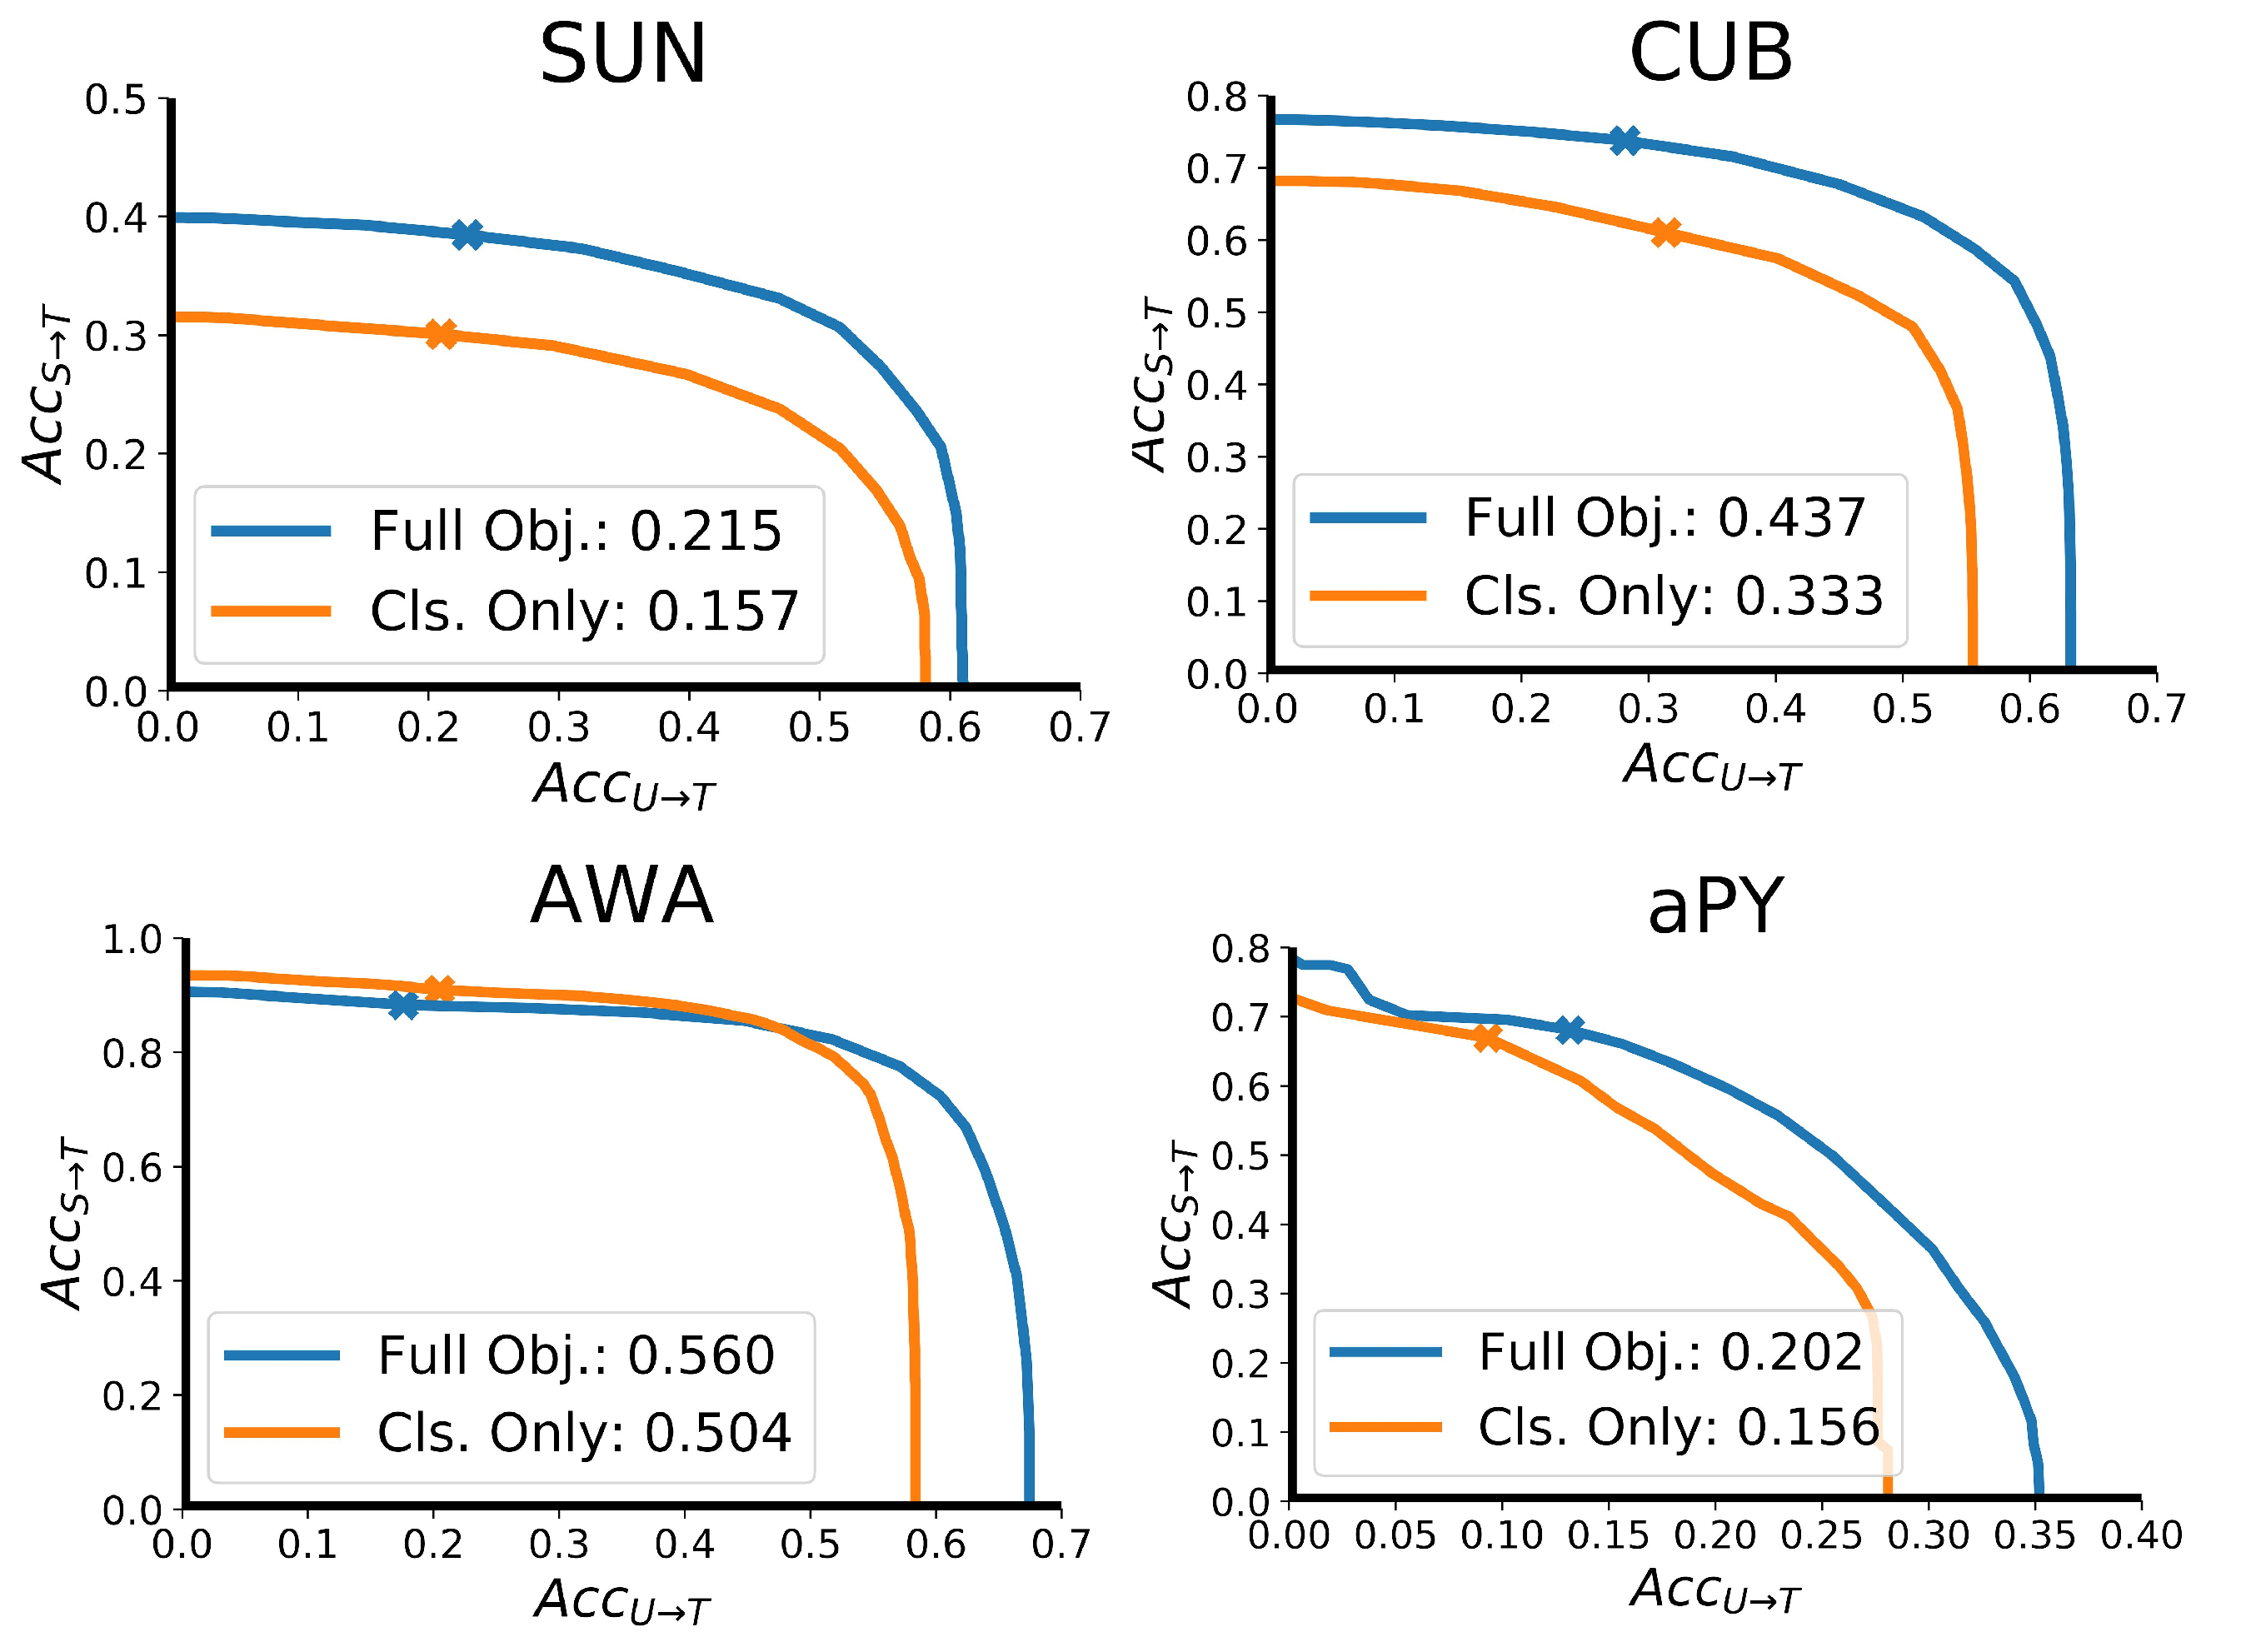
\includegraphics[width=0.8\linewidth]{chapter3/res/ausuc.pdf}
    \caption{在数据集SUN、CUB、AWA和aPY中的已见-未见准确率曲线下区域面积~\cite{chao2016empirical}}
\label{ch3:fig:ausuc}
\end{figure}


xxxx


\section{本章小结}

本章提出了一个全新的零样本分类框架:属性保持的对抗网络学习(SP-AEN),用于解决目前零样本分类模型中普遍存在的语义损失的问题。SP-AEN主要通过两个设计来解决语义损失问题:(1)引入一个独立的重建网络,同时重建网络不直接影响分类网络的优化目标。(2)通过对抗学习,实现重建语义向量和分类语义向量之间的知识迁移。我们通过大量的实验对比在四个标准数据集上验证了SP-AEN的性能。


\chapter{基于反事实多智能体学习的图像场景图生成方法}

图像场景图(scene graph)是将图像中每个物体当成一个节点,两两物体之间的视觉关系看成节点间的有向边,即视觉三元组“主语(物体)$\to$谓语(视觉关系)$\to$宾语(物体)”。图像场景图描绘了整个图像视觉场景中所有物体的类别、位置以及物体间的交互。为了生成准确的场景图,现有的场景图生成方法几乎都是通过“信息传递机制”(message passing),让每个物体和视觉关系都能充分地考虑和融合周围的视觉信息。例如,物体“人”和物体“自行车”之间一个最常见的视觉关系就是“骑”(即“人$\to$骑$\to$自行车”);同样,视觉关系“骑”也能够提升这两个物体(“人”和“自行车”)的类别预测概率。最后,这些方法都是直接利用物体和视觉关系分类的交叉熵之和作为模型最终的优化目标。然而,这个优化目标(交叉熵之和)将所有节点分类的重要性看成完全相同,即每个不同节点的分类损失对总的损失函数影响相同,这将大大限制模型融合周围信息的能力。

在本章,我们提出一种全新的反事实多智能体学习方法(Counterfactual critic Multi-Agent Training, CMAT)。模型CMT是一种基于多智能体策略梯度优化方法。它通过将每个物体看成一个智能体,从而将图像场景图生成任务转换成一个多智能体协同决策问题。基于这种转换,模型CMAT就可以直接利用整体场景图的生成质量作为优化目标(即全局奖励函数)。与此同时,为了给每个智能体分配适当的奖励,我们设计来一个反事实基准模型(counterfactual baseline)。这个反事实基准模型通过改变目标智能体的预测类别,同时固定其他所有智能体的预测,来推测当前智能体预测的局部贡献。通过在图像场景图生成数据集Visual Genome上进行大量的对比实验,模型CMAT在多个设定和评价指标下都达到当时最好的性能。


\section{问题描述}

视觉场景理解是计算机视觉研究领域一个重要的研究领域。它不仅仅需要对场景中所有物体的类别以及位置进行预测,同时需要对两两物体之间的视觉关系进行预测。随着目标检测~\cite{ren2015faster,liu2016ssd}与物体分割技术~\cite{long2015fully,he2017mask}的成熟,计算机已经可以准确地识别物体的类别、位置以及属性。然而,视觉场景理解不仅仅只是对单个物体的识别,还需要进一步对物体间视觉关系进行识别。所有的物体和视觉关系组合在一起,就构成了场景图~\cite{johnson2015image}。如图~\ref{ch4:fig:sgg}所示,场景图中每个节点和边分别表示图像中的物体和对应物体间的视觉关系。与此同时,图像场景图通常作为一种结构化的视觉知识,辅助许多视觉场景理解任务,如:图像描述生成~\cite{yao2018exploring,yang2019auto,kim2019dense}、视觉问答~\cite{norcliffe2018learning,hudson2019gqa}和视觉推理~\cite{shi2019explainable,haurilet2019s}等。

\begin{figure}[t]
    \centering
    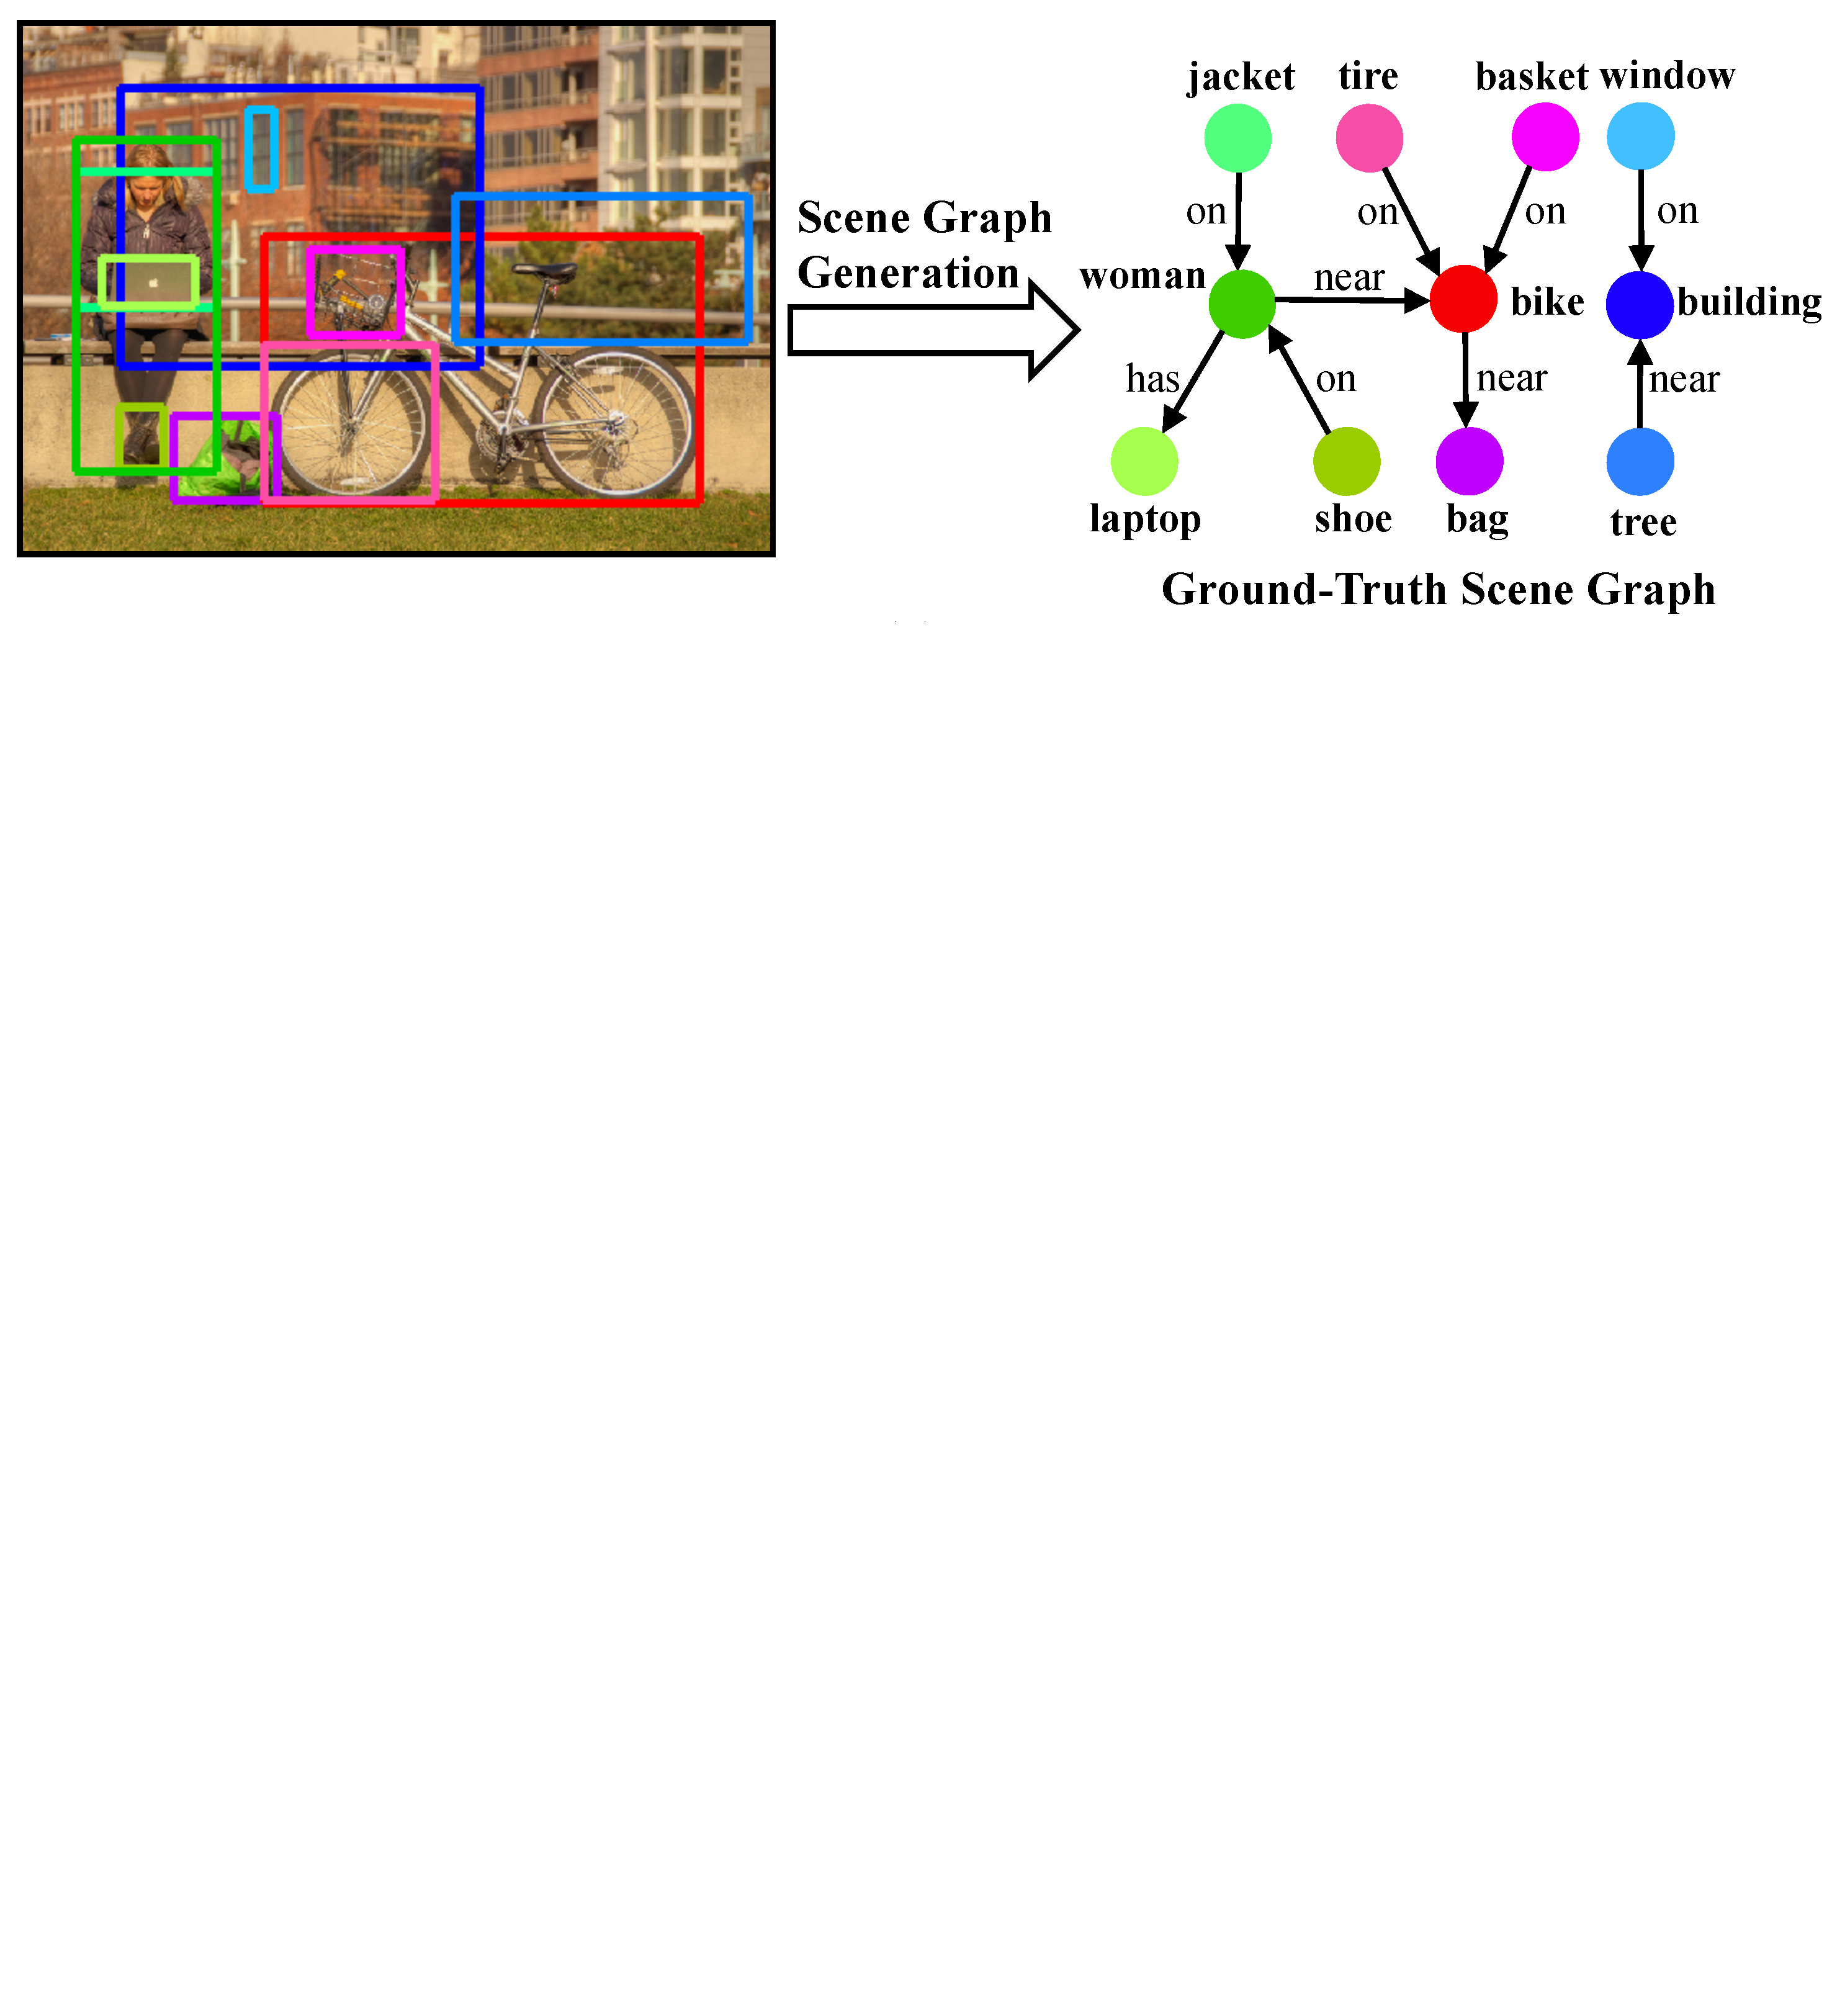
\includegraphics[width=0.95\linewidth]{chapter4/res/sgg.pdf}
    \caption{图像场景图生成任务示例}
    \label{ch4:fig:sgg}
\end{figure}

对于图像场景图生成任务(Scene Graph Generation, SGG),一个最直接的解决思路就是将场景图生成任务分解成物体分类和视觉关系分类两个独立的子任务,即先用一个物体检测器定位出物体框,然后分别预测每个物体框的类别以及两两物体框之间视觉关系的类别~\cite{lu2016visual,zhang2017visual,yang2018shuffle}。尽管这类方法的结构十分简单,但是它们都忽略了图像中所有视觉元素之间的内在联系,即每个物体(视觉关系)周围的视觉信息往往会提供一些归纳偏置~\cite{divvala2009empirical}(inductive bias)来辅助物体(视觉关系)的预测。如图~\ref{ch4:fig:sgg}所示,物体“窗户”(window)和物体“建筑物”(building)常常会出现在同一张图像中,“在附近”(near)也是物体“树”(tree)和物体“建筑物”(building)之间最常见的视觉关系类别。因此,从视觉关系三元组“窗户$\to$在上面$\to$?”或“树$\to$在附近$\to$?”中,很容易推测出物体“?”是“建筑物”。这些归纳偏置带来的辅助信息已经被广泛地用来提升场景图生成性能~\cite{xu2017scene, dai2017detecting, li2017vip, li2017scene, li2018factorizable, yin2018zoom, jae2018tensorize, zellers2018neural, tang2019learning, gu2019scene, qi2019attentive, wang2019exploring, qian2019video}。具体来说,这些方法都是通过借助条件随机场~\cite{zheng2015conditional}(Conditional Random Field, CRF)来建模所有节点和边的联合分布,然后通过信息传递机制来更新节点和边的特征~\cite{krahenbuhl2011efficient}。最后,整个模型利用所有节点(物体)和边(视觉关系)分类的交叉熵之和作为模型的优化目标进行参数优化。

\begin{figure}[t]
    \centering
    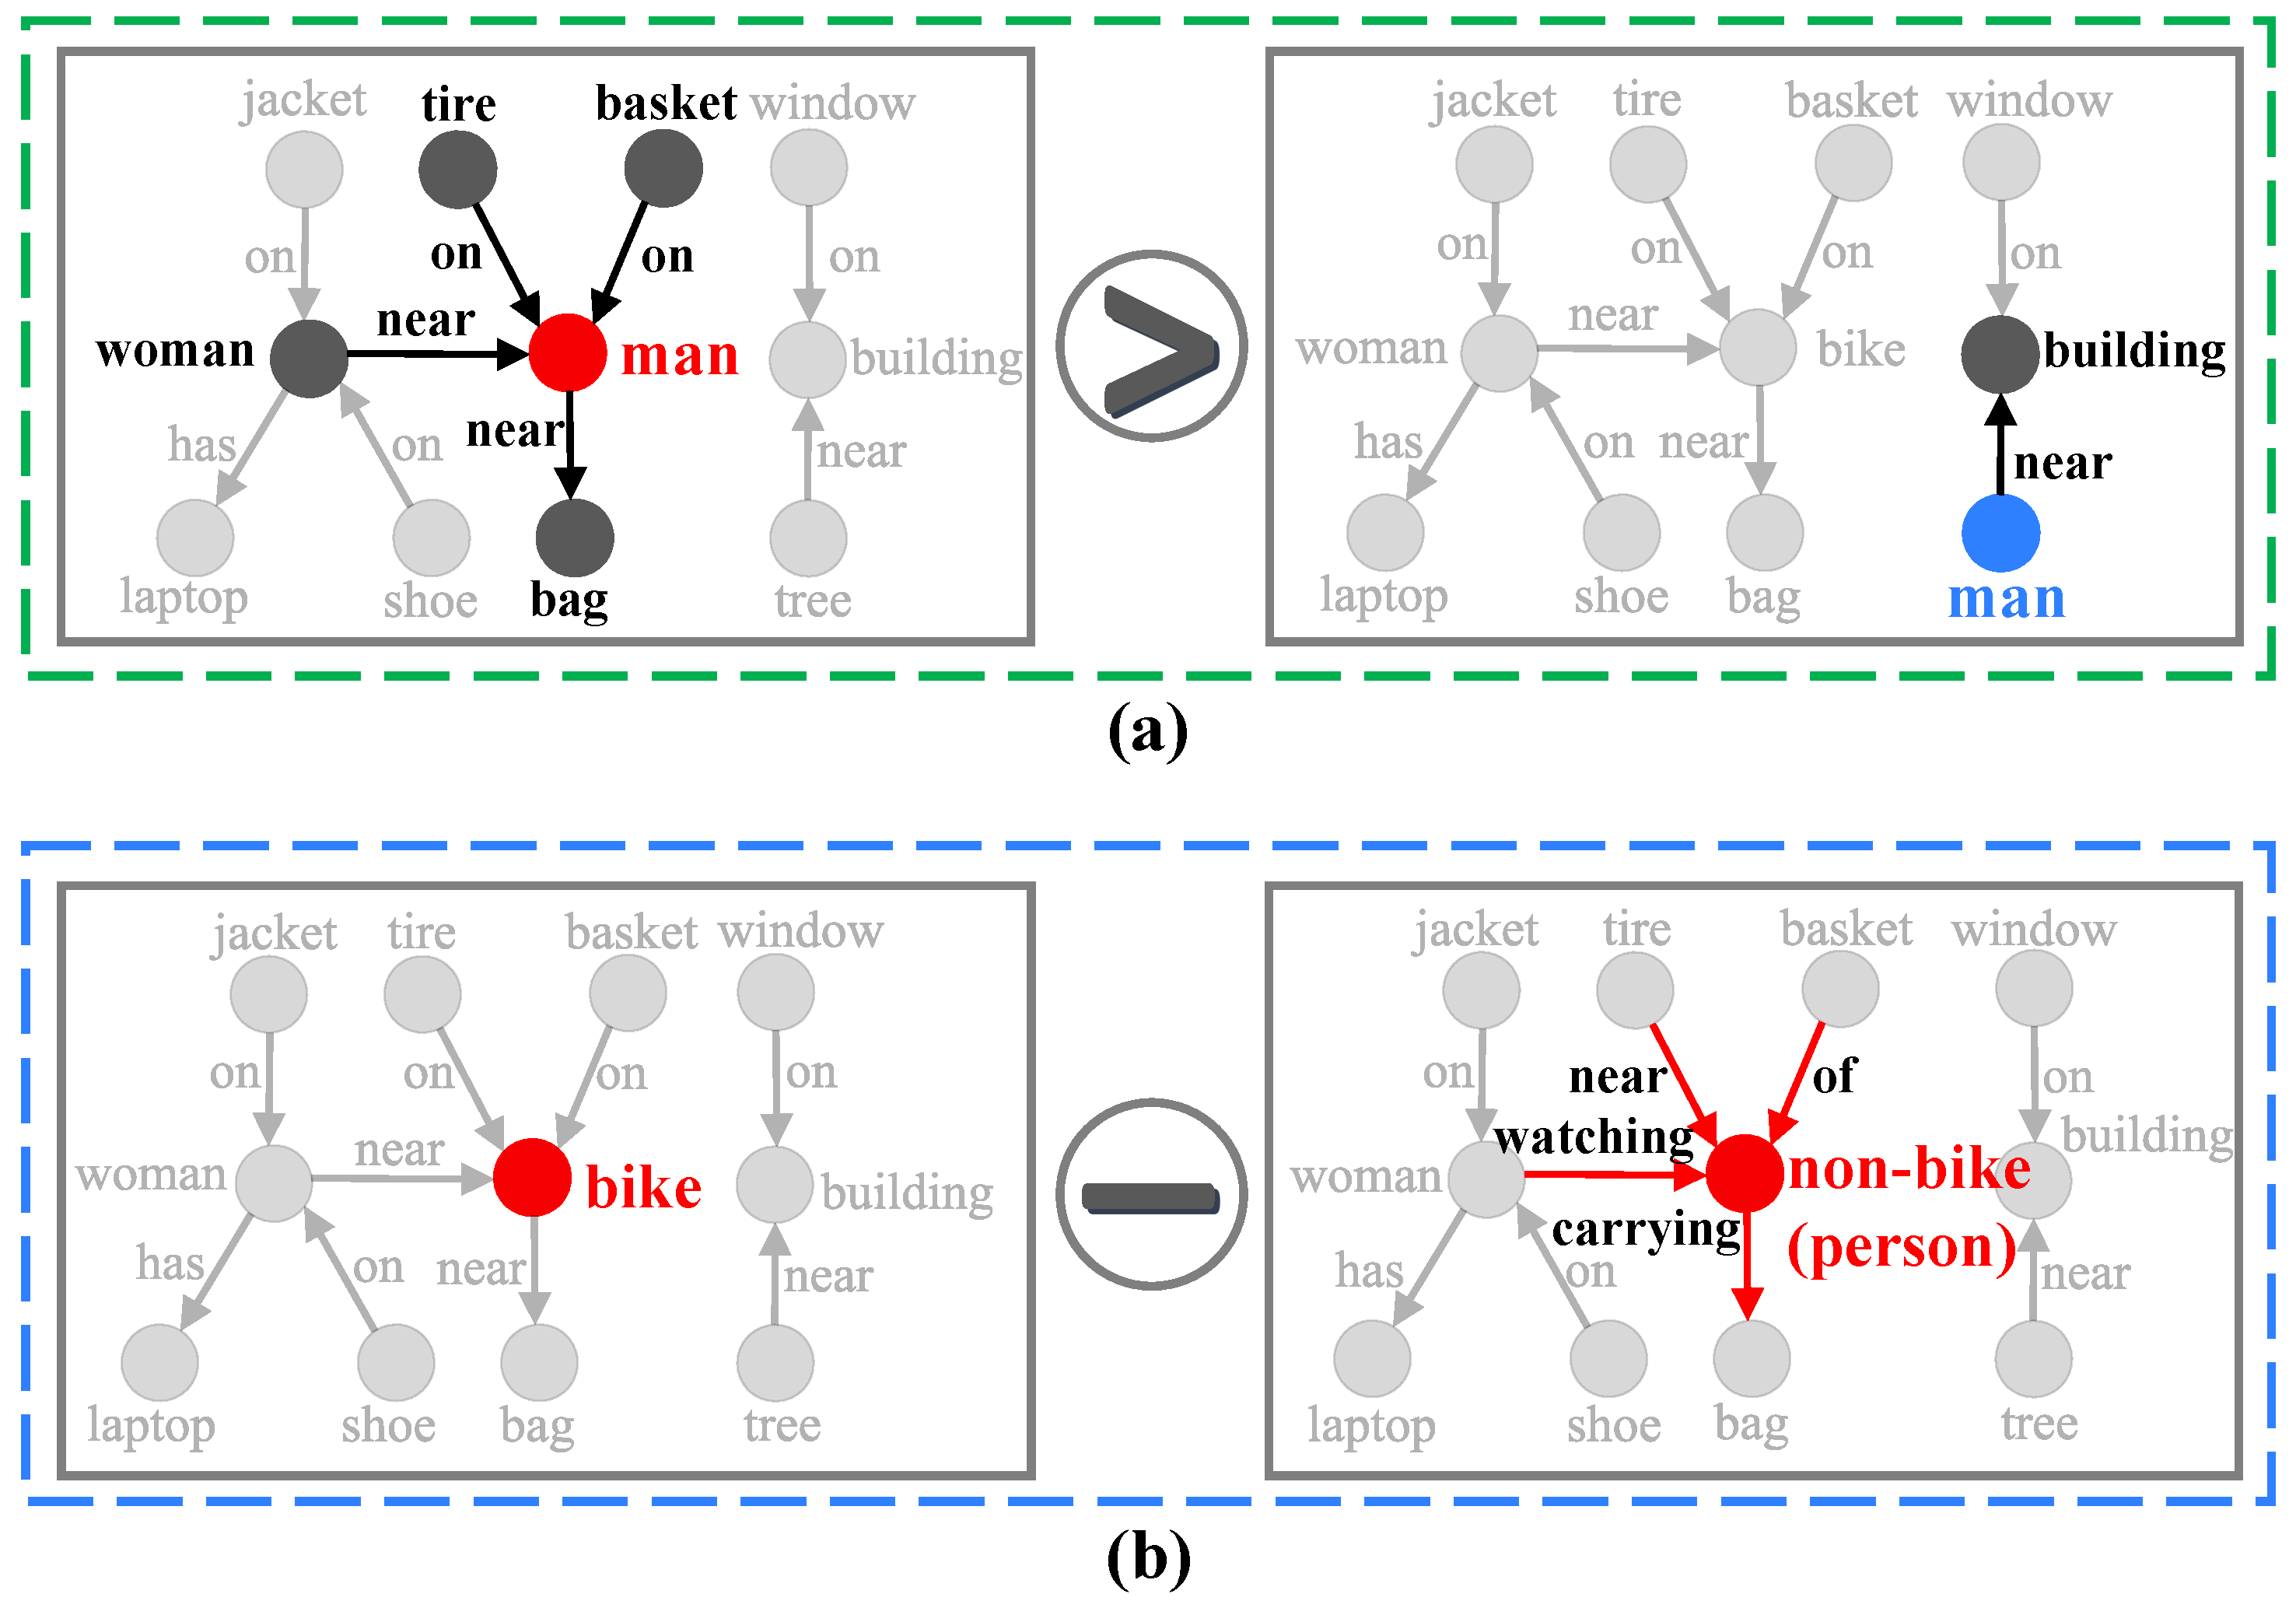
\includegraphics[width=0.95\linewidth]{chapter4/res/motivation.pdf}
    \caption{场景图生成中优化目标的整体一致性和局部敏感性}
    \label{ch4:fig:motivation}
\end{figure}

现有的图像场景图生成方法没有充分地利用场景中视觉元素之间的内在联系,一个重要的原因就是将物体和视觉关系分类的交叉熵之和作为场景图生成的优化目标。这个优化目标不具备\textbf{整体一致性}。所谓的“整体一致性”是指所有预测的物体类别和视觉关系类别之间应该保持整体一致。而交叉熵之和将所有的物体和视觉关系的预测看成是相互独立的。如图~\ref{ch4:fig:motivation}(a)所示,考虑两种极端情形,分别只有红色节点(“bike”)或蓝色节点(“tree”)被错误地分类成同一类别“man”,而其他所有的物体和视觉关系都正确。对于这两种情况,根据交叉熵之和的损失函数,它们最终的损失大小是完全相同的。然而,因为红色节点连接的边远多于蓝色节点,即对红色节点的错误分类将影响更多的视觉关系。因此,错误分类红色节点相比于错误分类蓝色节点应该导致更大的损失。因此,我们提出直接使用Recall@K~\cite{lu2016visual}或者SPICE~\cite{anderson2016spice}等图像场景图的全局评价指标作为优化目标。另一方面,场景图生成的优化目标还应该具备\textbf{局部敏感性}。所谓的“局部敏感性”是指优化目标应该能够感知每个节点类别的预测影响。由于场景图的全局评价指标是一个整体生成质量的评价数值,忽略了单个节点的预测贡献。因此我们需要设计一种机制,可以分解出每个节点各自预测的贡献,进而为每个局部预测计算更加有效的优化梯度。

在本章,我们提出了一种全新的场景图优化模型,可以同时满足优化目标的整体一致性和局部敏感性:反事实多智能体学习(CMAT)。具体来说,我们将图像场景图生成任务转换成一种多智能体协同决策任务。其中将每个物体看成是一个智能体,每个智能体的动作空间是所有可选择的物体类别。每个智能体之间可以进行通信,来编码周围的视觉元素,提升智能体内部的特征表达。经过多轮智能体通信之后,我们再利用一个视觉关系预测模型来预测智能体之间的视觉关系,得到最终的场景图预测结果。通过与人工标注的场景图对比,得到一个全局的奖励。

为了优化目标的整体一致性,我们直接将整体场景图生成的评价指标(如:Recall@K或SPICE~\cite{anderson2016spice})作为全局奖励函数,并且使用策略梯度(policy gradient)的方法对参数进行优化~\cite{sutton2000policy}。从多智能体强化学习~\cite{tampuu2017multiagent,lowe2017multi}(Multi-Agent Reinforcement Learning, MARL)的观点来看,尤其是“演员-评论家”方法~\cite{lowe2017multi}(actor-critic),模型CMAT模型中视觉关系预测模型可以看成是评论家(critic),而物体类别的分类模型可以看成是策略网络(policy network)。为了优化目标的局部敏感性,对于每个智能体,我们都从全局奖励中减去一个特定的反事实基准~\cite{foerster2018counterfactual}。这个反事实基准模型通过改变目标智能体的预测类别同时固定其他智能体的预测类别,来推测目标智能体预测的局部贡献。如图~\ref{ch4:fig:motivation}(b)所示,为了得到红色节点预测为“自行车”(bike)的贡献,我们可以固定其他节点的预测,而将红色节点的预测替换成其他的“非自行车”(non-bike)类,如“人”(person)等。进而通过计算出这种反事实式的替换对整体的场景图生成效果带来多大的影响,推测红色节点预测为“自行车”类别的贡献。

为了更好地编码物体周围的视觉元素信息和物体间的内在联系,我们还设计了一种更加有效的智能体通信(agent communication)模型。相比于现有的信息传递机制~\cite{xu2017scene, li2017scene, jae2018tensorize, li2017vip, yin2018zoom, li2018factorizable},我们不再将视觉关系也看成节点进行信息传递和更新。基于这个设计,我们可以将智能体通信与视觉关系分类两个任务分离出来,让前者关注如何编码物体周围视觉元素的内在联系,让后者作为评论家(critic)提供全局奖励来引导整个模型的优化。

我们在目前最大的图像场景图生成数据集Visual Genome上对模型CMAT的性能进行了验证。通过大量的对比实验,我们在通用的三种不同的实验设定下都可以达到当时最好的效果。

在本章,我们主要有三个技术贡献:

1)我们提出了一种全新的图像场景图生成模型的训练方法:反事实多智能体学习(CMAT)。据我们了解,我们是第一次将图像场景图生成任务转换成一个多智能体协同决策问题,使得优化目标满足整体一致性要求。

2)我们设计了一个全新的反事实基准模型,可以使得多智能体策略梯度算法的优化目标同时具备局部敏感性。

3)我们设计了一个有效的多智能体通信模型,有效地将智能体通信与视觉关系预测两个任务分离出来。


\section{反事实多智能体学习}
给定一个物体类别集$\mathcal{C}$(包括背景)和一个视觉关系类别集$\mathcal{R}$(包括没有视觉关系),图像场景图可以表示成:$\mathcal{G} = \left\{ \mathcal{V}=\{(v_i, \bm{l}_i)\},\mathcal{E}=\{r_{ij}\} | i,j = 1...n \right\}$,其中$\mathcal{V}$和$\mathcal{E}$分别表示所有节点(物体)和边(视觉关系)的集合。$v_i \in \mathcal{C}$表示第$i$个节点的物体类别,$\bm{l}_i \in \mathbb{R}^4$表示第$i$个节点的物体位置,$r_{ij} \in \mathcal{R}$表示第$i$个节点和第$j$个节点之间的视觉关系。图像场景图生成任务就是检测出图像中所有的物体以及物体间的视觉关系。

在本节,我们先介绍模型CMAT中的每个组成部分。然后,我们再介绍模型CMAT的优化目标。

\begin{figure}[t]
    \centering
    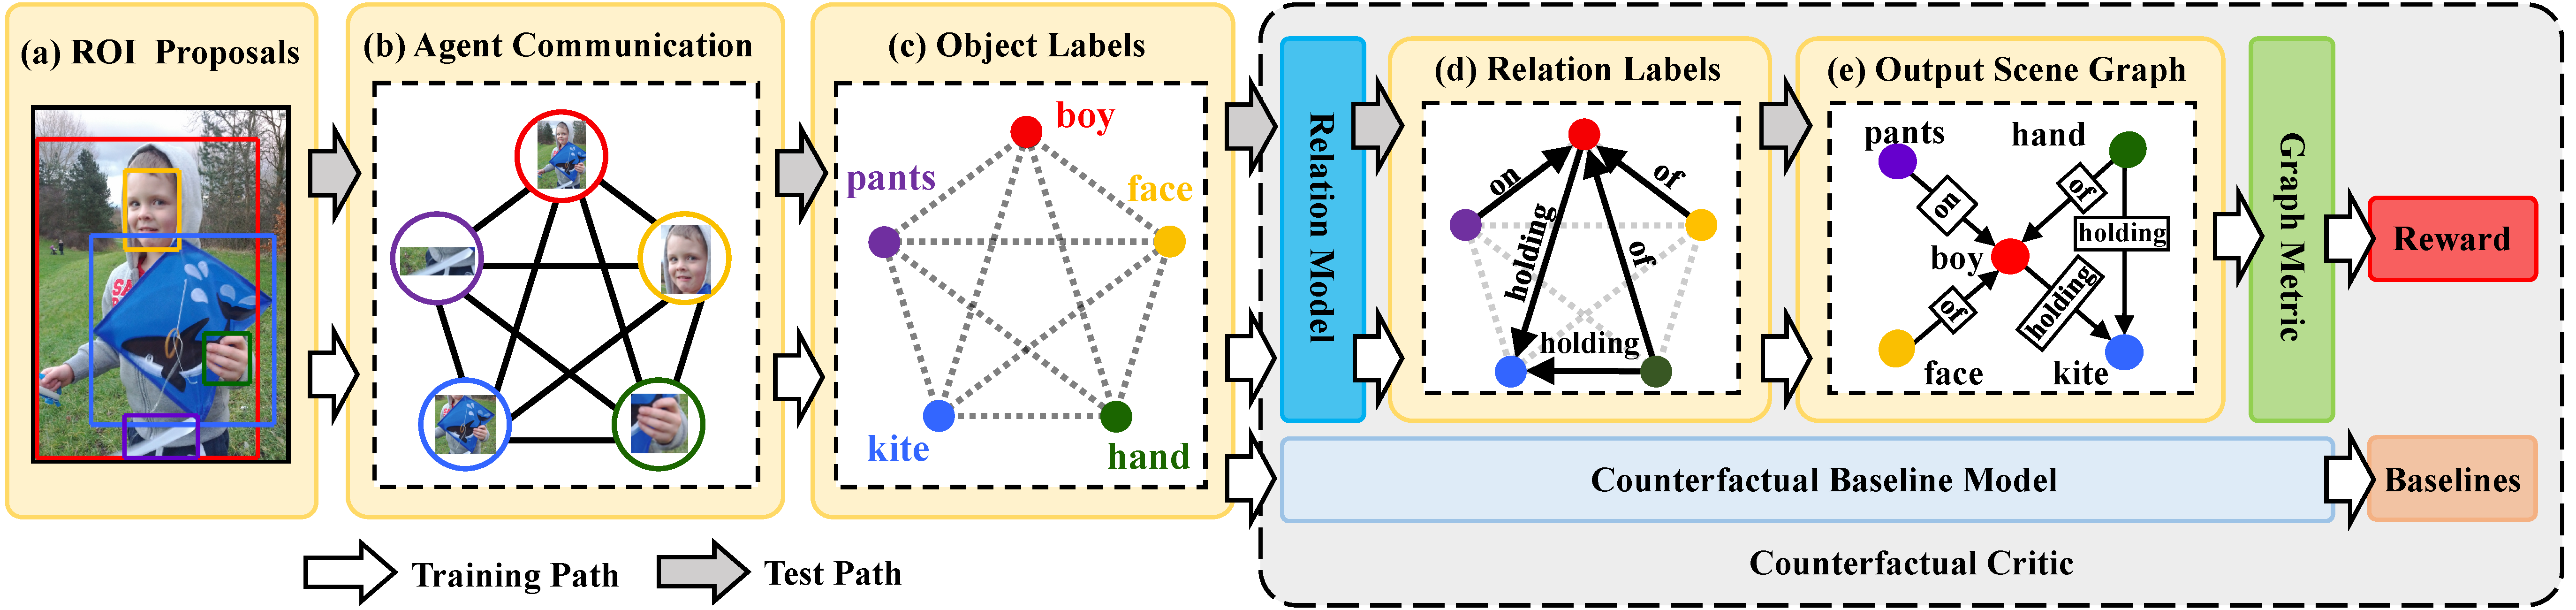
\includegraphics[width=\linewidth]{chapter4/res/architecture.pdf}
    \caption{模型CMAT的总体流程图}
    \label{ch4:fig:architecture}
\end{figure}

\subsection{多智能体协同决策模型}

\textbf{\kaishu{物体候选框检测}}:我们首先使用预训练好的目标检测器Faster R-CNN~\cite{ren2015faster}对输入图像进行物体检测,得到一系列候选框。对于每个候选框,我们可以同时得到其位置坐标$\bm{l}_i$、特征向量$\bm{x}^0_i$、以及初始的物体类别预测概率分布$\bm{s}^0_i$。上角标$0$表示$T$轮智能体通信的初始输入(第0轮)。我们参考现有的场景图生成工作~\cite{xu2017scene, zellers2018neural},固定所有候选框的位置$\{\bm{l}_i\}$作为物体位置的最终预测结果。为了后续表达的简洁性,我们在后续内容中省略位置坐标$\bm{l}_i$。


\textbf{\kaishu{智能体通信}}:给定$n$个物体候选框,我们将每个候选框看成是一个智能体。智能体之间将通过$T$轮的通信来编码每个物体与各自周围的视觉元素之间的内在联系。如图~\ref{ch4:fig:communication}所示,在单步智能体通信过程中,共有三个模块参与智能体通信:信息提取模块(extract module)、信息合成模块(message module)和状态更新模块(update module)。为了减小整个CMAT模型的参数量,这三个模块在所有的智能体之间都共享参数。关于这三个模块的具体细节如下:

\begin{figure}[t]
    \centering
    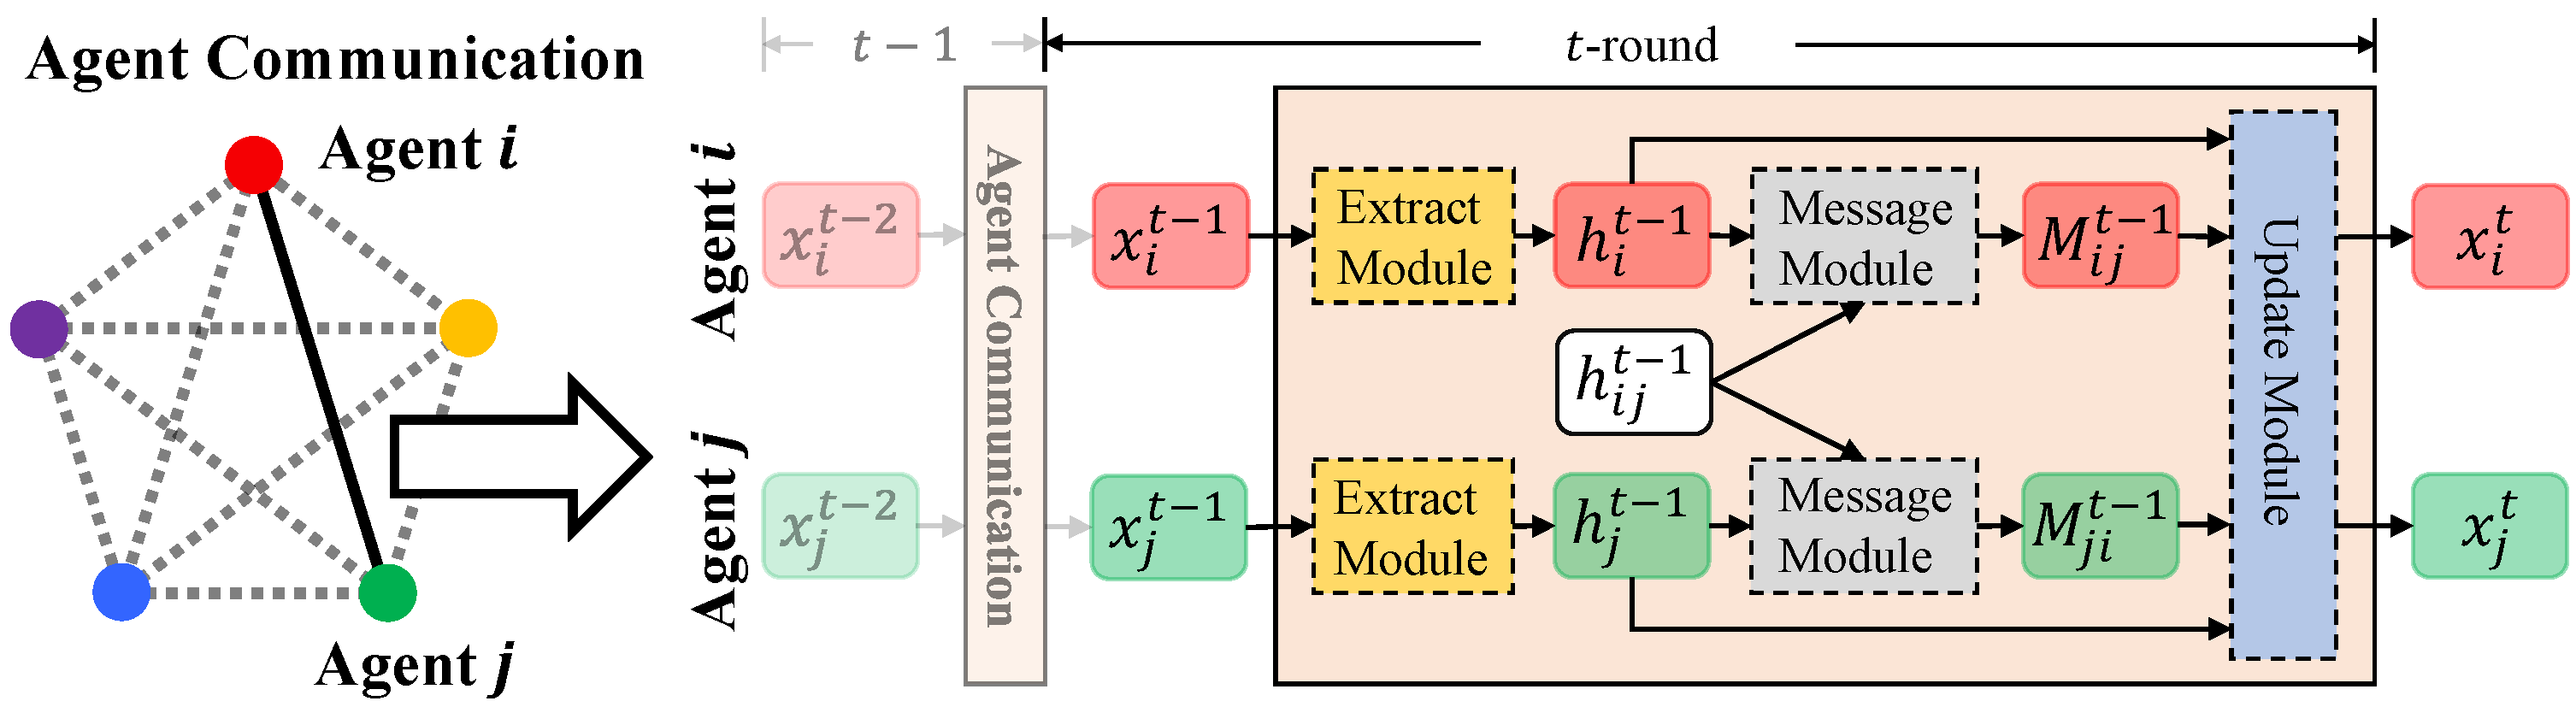
\includegraphics[width=\linewidth]{chapter4/res/communication.pdf}
    \caption{模型CMAT中的单步智能体通信示意图}
    \label{ch4:fig:communication}
\end{figure}

(a)信息提取模块:我们使用递归神经网络LSTM~\cite{hochreiter1997long}来实现信息提取模块。LSTM不仅可以编码智能体之间的交互历史,同时也可以提取智能体自身的内部状态。具体来说,对于第$i$个智能体,在第$t$轮($0 < t \leqslant T$)通信时:
\begin{equation}
\begin{aligned}
    \bm{h}^{t}_i & = \text{LSTM}(\bm{h}^{t-1}_i, [\bm{x}^{t}_i, \bm{e}^{t-1}_i]), \\
    \bm{s}^t_i & = \bm{s}^{t-1}_i + \bm{W}_h \bm{h}^{t}_i, \\
    v^t_i & \sim \bm{p}^{t}_i = \text{softmax}(\bm{s}^t_i), \\
    \bm{e}^{t}_i &= \textstyle{\sum_{\tilde{v}}} \bm{p}^{t}_i(\tilde{v}) \mathbf{E}[\tilde{v}],
\end{aligned}
\end{equation}
其中$\bm{h}^t_i \in \mathbb{R}^h$是LSTM的隐含状态向量,$\bm{x}^t_i \in \mathbb{R}^d$是每个LSTM时刻的输入特征,$\bm{s}^t_i \in \mathbb{R}^{|\mathcal{C}|}$是预测的物体类别概率分布。初始的(即第0步通信时)输入特征和类别预测概率都来自于物体候选框检测。$\mathbf{E}[\tilde{v}] \in \mathbb{R}^e$是类别标签$\tilde{v} \in \mathcal{C}$的特征编码向量,以及$\bm{e}^{t}_i \in \mathbb{R}^e$是一个基于类别概率$\bm{p}^t_i$加权的类别标签编码向量,$\bm{W}_h \in \mathbb{R}^{h \times |\mathcal{C}|}$是一个可学习的映射矩阵,以及$[,]$是向量间的连接操作。所有的隐藏状态$\{\bm{h}^t_i\}$都输入到之后的信息合成模块用于合成通信信息。


(b)信息合成模块:对于第$i$个智能体和第$j$个智能体之间的通信,信息合成模块将分别合成信息$M^t_{ij}$和$M^t_{ji}$。具体来说,对于第$i$个智能体收到的信息$M^t_{ij} = (\bm{m}^t_j, \bm{m}^t_{ij})$,主要包含两部分:
\begin{equation}
\begin{aligned}
\bm{m}^t_j = \bm{W}_u \bm{h}^t_j, \; \bm{m}^t_{ij} = \bm{W}_p\bm{h}^t_{ij},
\end{aligned}
\end{equation}
其中$\bm{m}^t_j \in \mathbb{R}^h$表示一元信息,用来表征第$j$个智能体本身的属性(如:单个物体的局部视觉特征),$\bm{m}^t_{ij} \in \mathbb{R}^h$表示二元信息,用来表征两个智能体之间的交互信息(如:两个智能体的相对位置信息)。$\bm{h}^t_{ij} \in \mathbb{R}^d$表示第$i$个智能体与第$j$个智能体之间的共同特征,它的初始化是两个智能体物体框合并之后的视觉特征。对于第$i$个智能体,所有来自其他智能体的通信信息$\{M^t_{i*}\}$和其内部状态$\bm{h}^t_i$都输入到状态更新模块,更新其内部状态。

(c)状态更新模块:在每轮智能体通信过程中,对于每个智能体,我们使用注意力机制~\cite{chen2017sca}来融合不同智能体的通信信息:
\begin{equation}
\begin{aligned}
    u^t_j &= \bm{w}_u [\bm{h}^t_i, \bm{h}^t_j], \\ 
    u^t_{ij} &= \bm{w}_p [\bm{h}^t_i, \bm{h}^t_{ij}], \\
    \alpha^t_j & = \exp(u^t_j) / \textstyle{\sum_k} \exp(u^t_k), \\
    \alpha^t_{ij} & = \exp(u^t_{ij}) / \textstyle{\sum_k} \exp(u^t_{ik}), \\
    \bm{x}^{t+1}_i &= \bm{W}_x (\text{ReLU} (\bm{h}^t_i + \textstyle{\sum_j} \alpha^t_j \bm{m}^t_j +  \textstyle{\sum_j} \alpha^t_{ij} \bm{m}^t_{ij})), \\
    \bm{h}^{t+1}_{ij} &= \text{ReLU} (\bm{h}^t_{ij} + \bm{W}_s \bm{h}^{t+1}_i + \bm{W}_e \bm{h}^{t+1}_j),
\end{aligned}
\end{equation}
其中$\alpha^t_j$和$\alpha^t_{ij}$是不同信息融合的权重,$\bm{w}_u \in \mathbb{R}^{2h}$、$\bm{w}_p \in \mathbb{R}^{h+d}$、$\bm{W}_x \in \mathbb{R}^{h\times d}$、$\bm{W}_s \in \mathbb{R}^{h\times d}$和$\bm{W}_e \in \mathbb{R}^{h\times d}$这些都是需要学习的映射矩阵。


\textbf{\kaishu{视觉关系预测}}:在$T$轮智能体通信之后,所有的智能体都完成了状态更新。在测试阶段,对于所有的智能体,我们直接根据预测的分数$\bm{s}^T_i$来选取所有智能体的物体类别$v^T_i$。最后,我们再利用视觉关系预测模型对任意两个智能体之间进行视觉关系分类:
\begin{equation}
\begin{aligned}
    \bm{z}_i & = \bm{W}_o [\bm{h}^T_i, \mathbf{E}[v^T_i]], \\
    \bm{z}_j & = \bm{W}_o [\bm{h}^T_j, \mathbf{E}[v^T_j]], \\
    \bm{p}_{ij} & = \text{softmax} ([\bm{z}_i,  \bm{z}_j] \odot \bm{W}_r \bm{z}_{ij} + \bm{w}_{v^T_i, v^T_j}), \\
    r_{ij} & = \arg \textstyle{\max_{r \in \mathcal{R}}} \bm{p}_{ij}(r),
\end{aligned}
\end{equation}
其中$\bm{W}_o \in \mathbb{R}^{(h+e) \times z}$、$\bm{W}_r \in \mathbb{R}^{z\times 2z}$都是需要学习的映射矩阵,$\bm{z}_{ij} \in \mathbb{R}^z$是第$i$个智能体与第$j$个智能体之间预测的视觉关系特征,$\odot$是特征融合函数~\cite{zhang2018learning}: $\bm{x} \odot \bm{y} = \text{ReLU}(\bm{W}_x \bm{x} + \bm{W}_y \bm{y}) - (\bm{W}_x \bm{x} - \bm{W}_y \bm{y})^2$,$\bm{w}_{v^T_i, v^T_j} \in \mathbb{R}^{|\mathcal{C}|}$是基于VG数据集统计的视觉关系类别偏置~\cite{zellers2018neural}。 


\subsection{反事实多智能体学习}

在本节,我们将详细介绍模型CMAT中优化目标的细节,具体包括:(1)符合整体一致性的多智能体策略梯度算法;(2)符合局部敏感性的反事实评论家模型。


\textbf{\kaishu{优化目标的整体一致性}}:目前,几乎所有的场景图生成算法都是将所有物体和视觉关系分类的交叉熵之和作为模型的优化目标。对于一个预测的场景图($\hat{\mathcal{V}}, \hat{\mathcal{E}}$),如果人工标注的场景图为($\mathcal{V}^{gt}, \mathcal{E}^{gt}$),根据交叉熵之和(cross-entropy, XE)的优化目标,整个模型的损失函数则为:
\begin{equation} \label{ch4:eq:eq_5}
\begin{aligned}
   L(\theta) =  \textstyle{\sum_{ij}} \left(\text{XE}(\hat{v}_i, v^{gt}_i) + \text{XE}(\hat{r}_{ij}, r^{gt}_{ij}) \right). 
\end{aligned}
\end{equation}
由公式~\eqref{ch4:eq:eq_5}可以看出,交叉熵之和的优化目标本质上将所有的节点预测都看成相互独立的。

为了解决上述问题,我们提出将交叉熵之和的优化目标替换成以下两种具备整体一致性的优化目标:(1)\textbf{Recall@K}~\cite{lu2016visual}在预测分数最高的前K个视觉三元组(“主语$\to$谓语$\to$宾语”)中,预测正确的视觉三元组占所有标注视觉三元组的百分比。(2)\textbf{SPICE}~\cite{anderson2016spice}:所有视觉三元组预测的准确率和召回率之间的F值。与交叉熵之和不同的是,Recall@K和SPICE都是不可导的。因此,模型CMAT需要借助多智能体策略梯度算法对模型参数进行优化。


\textbf{\kaishu{多智能体策略梯度}}:
我们首先定义模型CMAT中智能体的动作(action)、策略函数(policy)和状态(state)。然后,我们推导出模型参数的梯度计算公式。

(a)动作:每个智能体的动作空间是所有可选择的物体类别的集合,即第$i$的智能体的动作是$v^t_i$。我们用集合$V^t = \{v^t_i\}$来表示所有智能体的动作集合。

(b)状态:我们参考Hausknecht等人~\cite{hausknecht2015deep}使用递归神经网络LSTM(信息提取模块)来编码智能体与环境之间的交互历史(history)。LSTM的隐含状态$\bm{h}^t_i$可以看成是第$i$个智能体对局部可见环境状态的近似。我们用集合$H^t = \{\bm{h}^t_i\}$来表示所有智能体的状态集合。

(c)策略函数:每个智能体的策略函数就是物体类别分类模型。在训练阶段,每个智能体通过对分类概率进行采样得到智能体类别,即:$\bm{p}^T_i = \text{softmax}(\bm{s}^T_i)$。因为模型CMAT只在$T$轮智能体通信之后进行动作采样,根据策略梯度的理论~\cite{sutton2000policy},模型CMAT中梯度计算公式为:
\begin{align}
\nabla_{\theta} J \approx \sum^n_{i=1} \nabla_{\theta} \log \bm{p}^T_i (v^T_i|h^T_i; \theta)Q(H^T, V^T),
\end{align}
其中,$Q(H^T, V^T)$为状态-动作函数(state-action value function)。不同于现有的演员-评论家~\cite{bahdanau2017actor,lowe2017multi,konda2000actor}(actor-critic)算法通常用一个独立的网络来近似函数$Q$,在模型CMAT中,我们参考Rao等人~\cite{rao2018learning}直接使用实际的奖励来代替函数$Q$。这样做的原因主要有两个:(1)在图像场景图生成任务中,智能体的数量(如:SGDet中通常检测64个物体框)和动作空间的采样大小(如:数据集VG中有150个物体类别)都明显大于现有的多智能体策略梯度的工作。这容易导致训练样本不充足,难以训练一个准确的状态-动作函数。(2)直接使用实际的奖励可以大大减小模型的复杂度,提升模型训练速度。因此,模型CMAT中梯度计算公式变为:
\begin{align} \label{ch4:eq:eq_7}
\nabla_{\theta} J \approx \sum^n_{i=1} \nabla_{\theta} \log \bm{p}^t_i (v^T_i|h^T_i; \theta) R(H^T, V^T),
\end{align}
其中,$R(H^T, V^T)$是实际的全局奖励(即:Recall@K或SPICE)。另外,值得注意的是,$R(H^T, V^T)$里包含一个可以学习的视觉关系分类模型。

\begin{figure}[t]
    \centering
        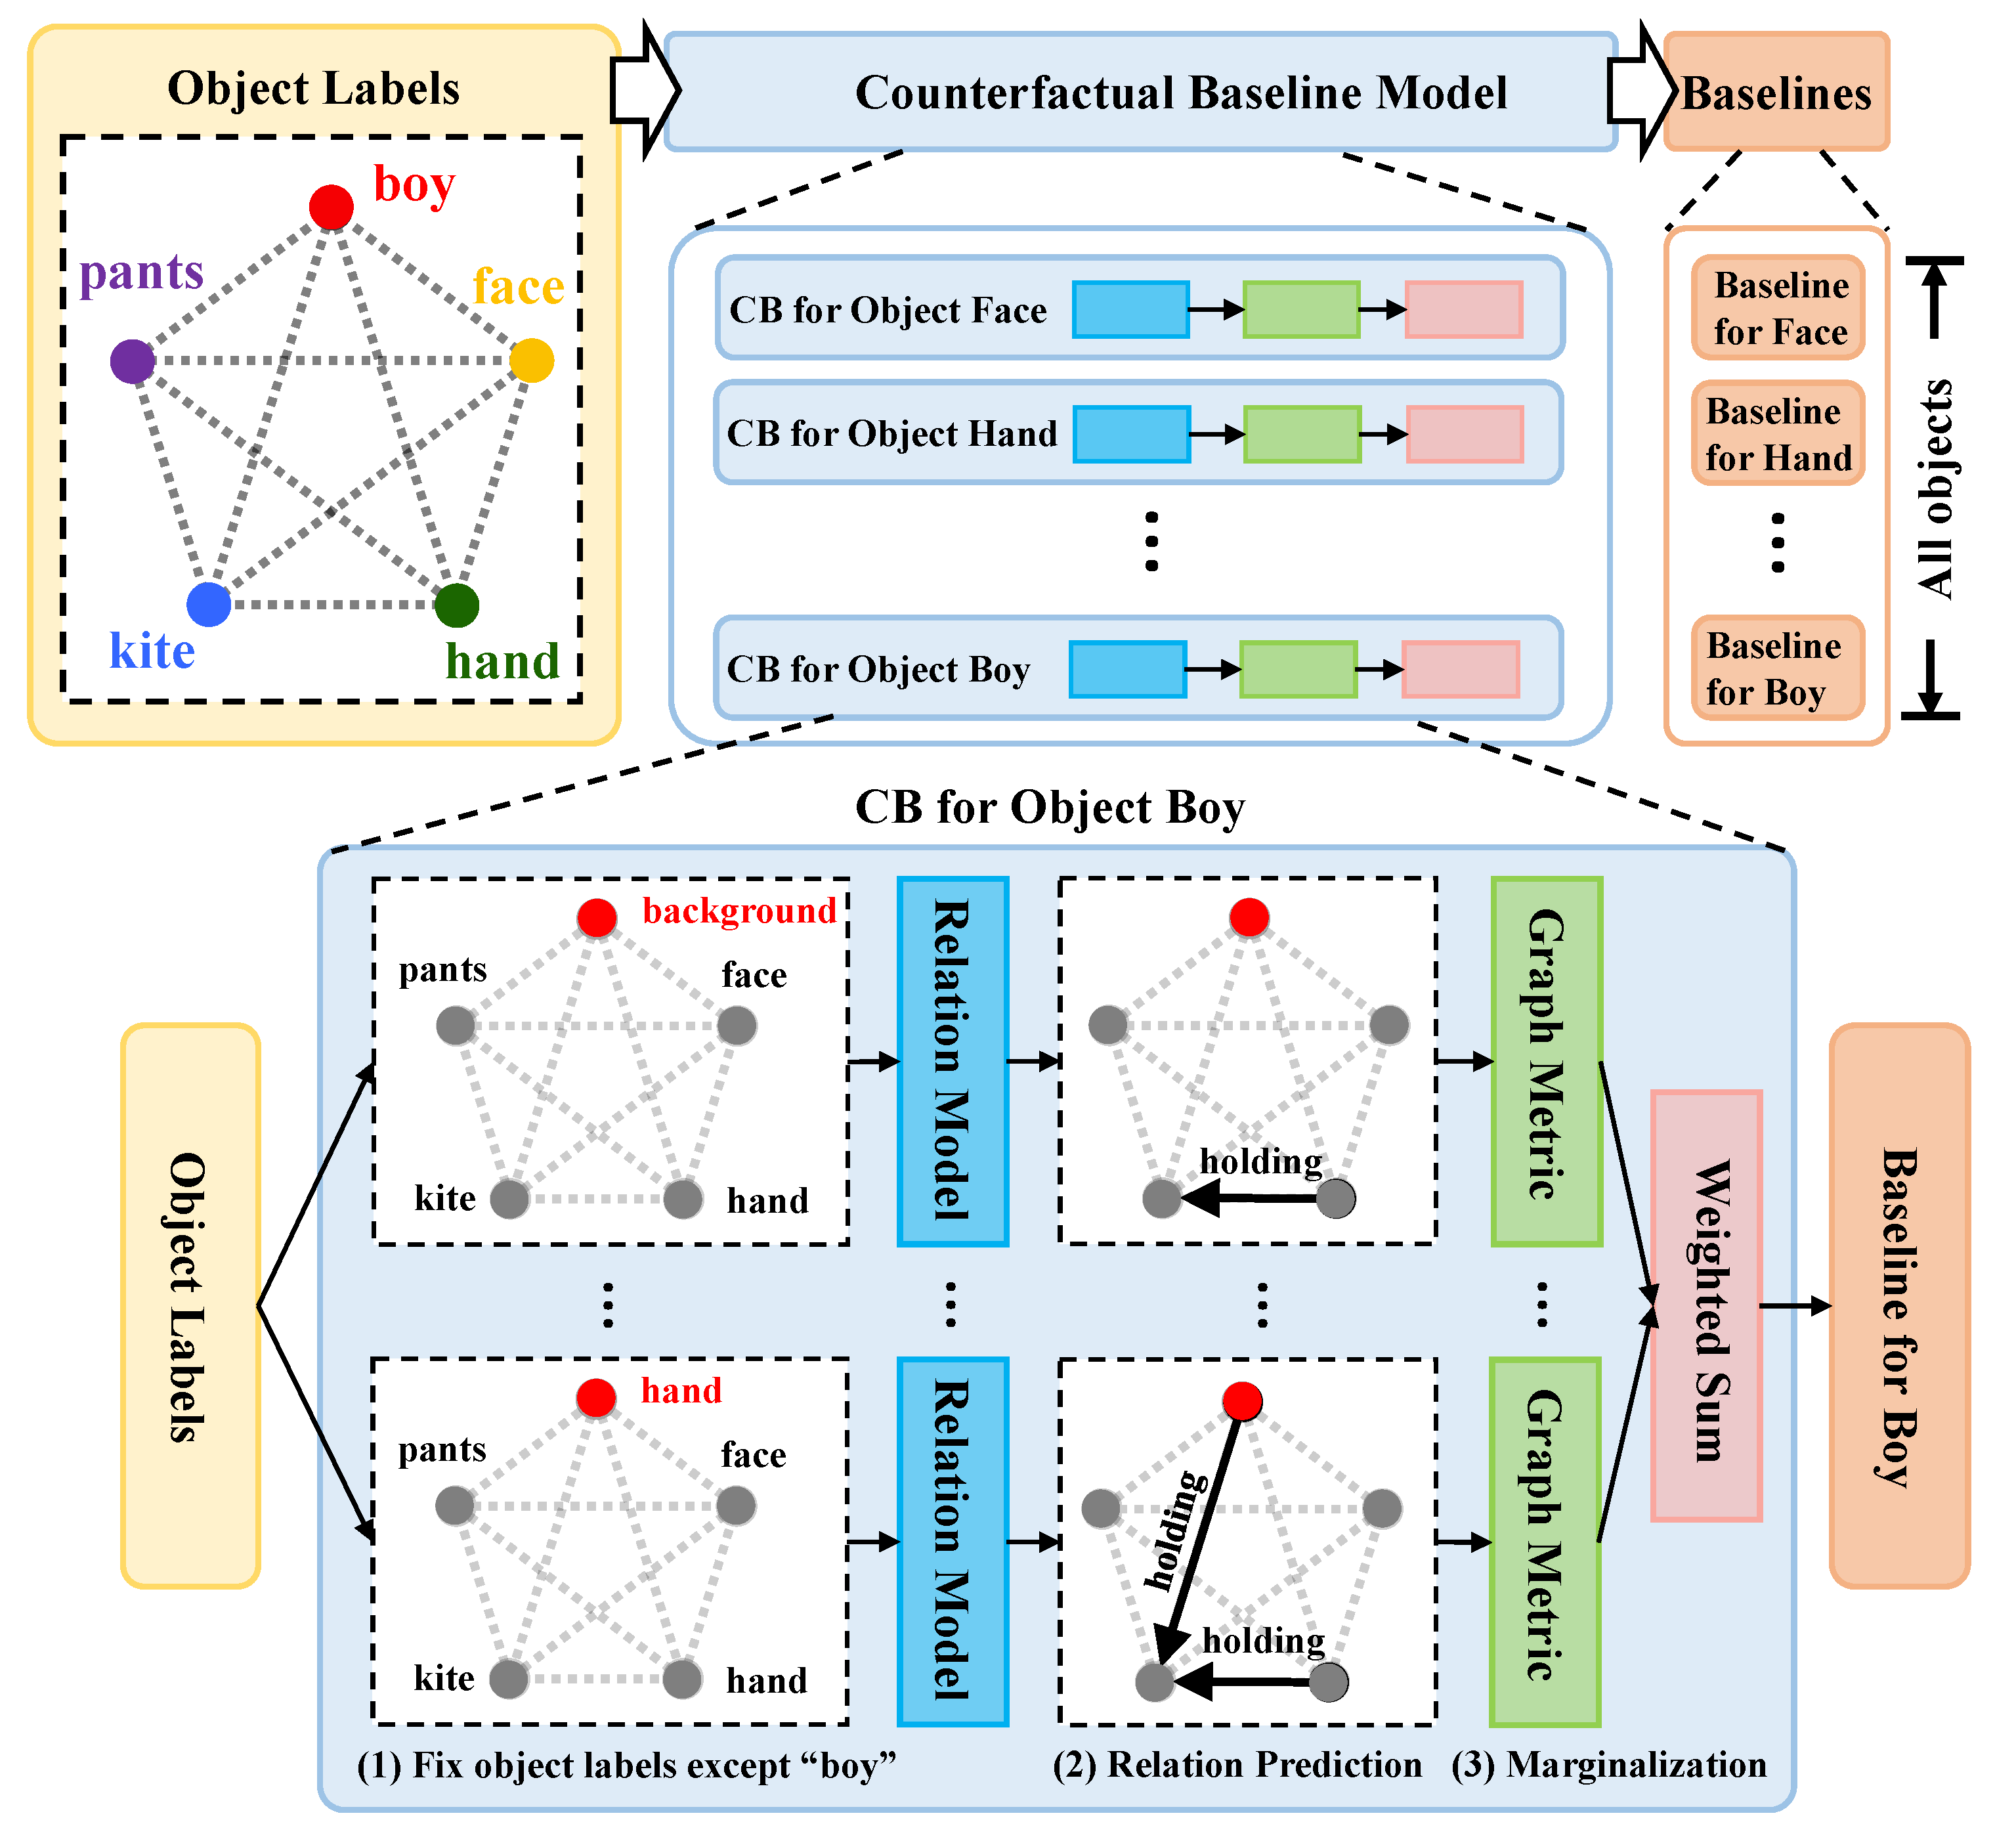
\includegraphics[width=0.95\linewidth]{chapter4/res/baseline.pdf}
    \caption{模型CMAT中反事实基准模型}
    \label{ch4:fig:baseline}
\end{figure}


\textbf{\kaishu{优化目标的局部敏感性}}:从上述公式~\eqref{ch4:eq:eq_7}可以看出,全局的奖励是综合考虑了所有智能体预测类别的总贡献,即对每个单独的智能体而言,总贡献是完全相同的。在图~\ref{ch4:fig:local_sensitive}中,我们用一个简单的示例来说明这种“总贡献”对场景图生成任务的副作用。如图~\ref{ch4:fig:local_sensitive}所示,绿色和红色分别表示正确的预测和错误的预测(包括节点和边),假定全局奖励函数定义为预测正确的视觉三元组数减去预测错误的视觉三元组数,且在图~\ref{ch4:fig:local_sensitive}(1)(2)两个场景图中只有节点“a”预测不同,其他预测都完全相同。

\begin{wrapfigure}{r}{0.55\linewidth}
    \centering
        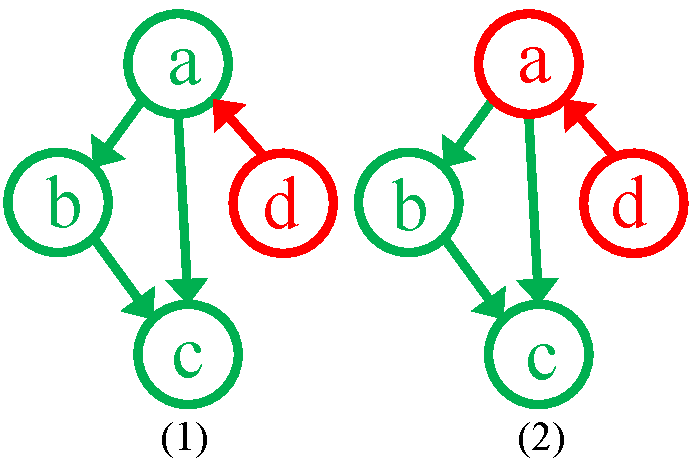
\includegraphics[width=0.9\linewidth]{chapter4/res/local_sensitive.pdf}
    \captionof{figure}{优化目标局部敏感性的重要性示例图}
    \label{ch4:fig:local_sensitive}
\end{wrapfigure}

根据公式~\eqref{ch4:eq:eq_7},场景图(1)中所有的节点都得到一个正的全局奖励(3-1=+2),而场景图(2)中所有的节点都得到一个负的全局奖励(1-3=-2)。在这两种情况下,虽然节点“b”、“c”、“d”的预测完全相同,但是对于它们计算得到的梯度方向却完全相反,容易造成模型多次无效的优化迭代。因此,通过让优化目标满足局部敏感性,即通过计算每个智能体各自的局部奖励,有利于提供更有效的优化梯度,提升模型训练效率。

\textbf{\kaishu{反事实评论家}}:一个直观地计算某个智能体动作的局部奖励的方法就是将目标智能体的动作替换成其他的动作,然后利用总贡献的变化来近似。因此,$R(H^T, V^T) - R(H^T, (V^T_{-i}, \tilde{v}^T_i))$可以表示第$i$个智能体的动作$v^T_i$的局部贡献,其中$V^T_{-i}$表示除第$i$个智能体以外其他所有智能体都保持初始的预测动作,而第$i$个智能体采取新的动作$\tilde{v}^T_i$。由于新的动作$\tilde{v}^T_i$有$|\mathcal{C}|$种可能性,为了准确地计算其他所有智能体动作(即:$V^T_{-i}$)的贡献,我们对所有可能的动作进行平均:$ \text{CB}^i(H^T, V^T) = \sum \bm{p}^T_i(\tilde{v}^T_i) R(H^T, (V^T_{-i}, \tilde{v}^T_i))$,其中$\text{CB}^i(H^T, V^T)$称为第$i$个智能体的\textbf{反事实基准}(counterfactual baseline)。这个反事实基准表示的意义是无论第$i$个智能体采用的动作,其他所有智能体采用默认动作时模型能够得到的平均全局奖励。模型CMAT的反事实基准模型展示在图~\ref{ch4:fig:baseline}中。

给定一个全局的奖励$R(H^T, V^T)$和第$i$个智能体动作的反事实基准$\text{CB}^i(H^T, V^T)$,我们可以得到第$i$个智能体动作的局部贡献为:
\begin{align}
    A^i(H^T, V^T) = R(H^T, V^T) - \text{CB}^i(H^T, V^T),
\end{align}
其中,$A^i(H^T, V^T)$在演员-评论家算法~\cite{sutton2018reinforcement,mnih2016asynchronous}中常被称为“优势”(advantage),$\text{CB}^i(H^T, V^T)$在策略梯度算法中常被称为“基准”(baseline),用来减少梯度计算时的方差。整个计算$A^i(H^T, V^T)$的网络结构可以合称为“反事实评论家”(counterfactual critic)。因此,根据公式~\eqref{ch4:eq:eq_7},模型CMAT的梯度计算公式变为:
\begin{align}
\nabla_{\theta} J \approx \sum^n_{i=1} \nabla_{\theta} \log \bm{p}^T_i (v^T_i|h^T_i; \theta) A^i(H^T, V^T).
\end{align}

最后,我们在加上交叉熵之和损失一起训练,最终参数训练的梯度为:
\begin{equation}
\begin{split}
\nabla_{\theta} J \approx  \overbrace{\sum^n_{i=1} \nabla_{\theta} \log \bm{p}^T_i (v^T_i|h^T_i; \theta) A^i(H^T, V^T)}^{\text{CMAT}} + \\
\underbrace{\alpha\sum^n_{i=1}\sum^n_{j=1} \nabla_{\theta} \log \bm{p}_{ij}(r_{ij})}_{\text{视觉关系交叉熵之和}} + 
\underbrace{\beta \sum^n_{i=1} \nabla_{\theta} \log \bm{p}^T_i(v^T_i)}_{\text{物体类别交叉熵之和}},
\end{split}
\end{equation}
其中,$\alpha$和$\beta$是不同损失函数之间权衡的权重,额外的交叉熵之和是为了增加模型训练的稳定性~\cite{rao2018learning}。同样,我们还增加了一个熵正则项~\cite{xu2015show, hu2017learning}来约束$\{\bm{p}^T_i\}_i$。


\section{实验设置与性能对比}
\subsection{图像场景图生成数据集与实验设定}

\textbf{\kaishu{图像场景图生成数据集}}:我们使用目前最大的图像场景图数据集Visual Genome~\cite{krishna2017visual}对模型性能进行评估。为了能够与现有的工作公平地进行比较,我们采用与它们完全相同的数据集划分和预处理步骤~\cite{xu2017scene, zellers2018neural, newell2017pixels, yang2018graph, herzig2018mapping}。处理后的数据集共包含150个物体类别和50个视觉关系类别。每张图像平均包含11.5个物体和6.2个视觉关系。在整个数据集中,70\%的图像作为训练集,剩余30\%的图像作为测试集。


\textbf{\kaishu{实验设定}}:我们参考现有的图像场景图生成的工作~\cite{xu2017scene, zellers2018neural, jae2018tensorize},在三种实验设定下评估场景图生成质量:
\begin{asparaenum}
\item \textbf{视觉关系分类(PredCls)}:给定图像中所有的物体框位置和物体类别,模型只需要预测两两物体间的视觉关系类别;

\item \textbf{场景图分类(SGCls)}:给定图像中所有的物体框位置,模型需要预测所有物体的类别以及两两物体间的视觉关系类别;

\item \textbf{场景图检测(SGDet)}:给定图像,模型需要检测物体框位置、预测物体类别以及两两物体间的视觉关系类别。
\end{asparaenum}

一个视觉三元组预测正确,不仅需要主语(subject)、谓语(predicate)和宾语(object)的类别都预测正确,同时需要主语和宾语的物体框与真实准确物体框的交并比(IoU)均大于0.5。按照图像场景图生成任务惯例,我们使用Recall@20(R@20)、Recall(R@50)和Recall(R@100)作为场景图生成质量的评价指标。

\subsection{实验细节}

\textbf{\kaishu{物体检测器}}:为了公平地与现有的工作进行对比,我们采用了与Zellers等人~\cite{zellers2018neural}完全相同的物体检测器。具体来说,它是以VGG网络~\cite{simonyan2015very}为主干网络,然后锚框的大小和长宽比与YOLO-9000~\cite{redmon2017yolo9000}设置一样, 然后用RoIAlign~\cite{he2017mask}代替RoIPooling~\cite{girshick2014rich,girshick2015fast}。

\textbf{\kaishu{训练细节}}:我们参照之前的策略梯度的工作,将整个训练过程分成两个阶段:先使用监督训练对模型参数进行初始化,再使用策略梯度对模型参数进行微调。在监督训练过程中,我们将RoIAlign层之前的参数都固定住,然后使用所有物体和视觉关系分类的交叉熵之和作为优化目标。批处理的大小和初始的学习率分别设为6和$10^{-3}$。在策略梯度优化过程中,初始的学习率设为$3\times5^{-5}$。对于场景图检测任务,因为所有可能的物体组合非常多(例如:64个物体框就存在大约4000中组合),我们参照Zellers等人~\cite{zellers2018neural}只考虑当物体有重叠时的视觉关系,这样可以将每张图预测的视觉关系数减少到1000左右。

\textbf{\kaishu{速度与正确率的权衡}}:在策略梯度的训练过程中,完整的反事实评论家的计算需要对所有可能的物体类别进行平均加权,通常需要非常多的时间(如:对于64个智能体,每个智能体共有151种物体类别选择,则需要超过9600次($\approx 151 \times 64$)计算评价指标Recall@K)。幸运的是,初始的目标检测器可以对物体类别有个初步的预测概率,而只有极少数的类别才有较大的预测概率,绝大多数类别的预测概率都趋近于0。为了速度与正确率之间的权衡,我们只对背景(background)和预测概率最高的两种类别进行平均求和来近似对所有的类别的期望。在我们的实验中,这样的实验简化可以减少70倍的评估计算,同时维持几乎相同的实验效果。

\textbf{\kaishu{SGDet的后处理}}: 对于场景图检测任务(SGDet),为了与之前的工作~\cite{zellers2018neural,zhang2019graphical}公平地进行对比,我们采用相同的后处理操作。具体来说,在对每个RoI预测出物体所有类别的概率分布之后,我们对每个类别使用一次非极大值抑制来确定最终的物体类别,以及选择对应类别的位移偏置。在我们的实验中,非极大值抑制的IoU阈值设置为0.5。


\subsection{场景图生成性能分析}
在本节,我们通过大量的对比实验来分析模型CMAT中的不同设计选择对总体性能的影响,包括全局奖励函数的选择、基准模型的选择、以及多智能体通信步数的选择等。

\textbf{\kaishu{全局奖励函数的选择}}:为了验证不同的全局奖励对最终场景图生成性能的影响,我们对比了两种全局奖励函数:\textbf{Recall@K}和\textbf{SPICE}。在这个实验中,我们使用预测前20个视觉三元组来计算对应的Recall@K和SPICE值。实验结果展示在表~\ref{ch4:tab:reward_choice}中,其中XE表示以所有物体和视觉关系交叉熵之和为优化目标的预训练结果。从表~\ref{ch4:tab:reward_choice}可以看出,全局奖励函数Recall@K和SPICE都能在交叉熵之和为优化目标的预训练基础上进一步提升场景图生成性能,这主要是因为将全局奖励函数作为场景图生成优化目标满足整体一致性。另外,使用Recall@K可以得到比SPICE稍微好一点的结果,可能的原因是因为目前的场景图生成数据集都是不完全标注的,而评价指标SPICE不适合用来评估这类数据集。因此,在后续的实验中,我们都使用Recall@K作为全局奖励函数。

%%%%%%%%%%%%%%%%% reward choice %%%%%%%%%%%%%%
\begin{table}[t]
\begin{center}
\scalebox{0.95}{
    \begin{tabular}{|l|l ccc|}
    \hline
    & & XE & R@20 & SPICE  \\
    \hline
    \multirow{2}{*}{SGCls} & R@20 & 34.08 & \textbf{35.93} & 35.27  \\
    & SPICE & 15.39 & \textbf{16.01} & 15.90 \\
    \hline
    \multirow{2}{*}{SGDet} & R@20 & 16.23 & \textbf{16.53} & 16.51  \\
    & SPICE & 7.48 & \textbf{7.66} & 7.64  \\
    \hline
    \end{tabular}
}
\end{center}
\caption{不同全局奖励函数对性能的影响}
\label{ch4:tab:reward_choice}
\end{table}
%%%%%%%%%%%%%%%%%%%%%%%%%%%%%%%%%%%%%%%%%%%%%%%%%%%%

%%%%%%%%%%%%%%%%% baseline types %%%%%%%%%%%%%%
\begin{table}[t]
\begin{center}
\scalebox{0.95}{
    \begin{tabular}{|l|l cccc|}
    \hline
    & & XE & MA & SC & CF  \\
    \hline
    \multirow{3}{*}{SGCls} & R@20 & 34.08 & 34.76 & 34.68 & \textbf{35.93} \\
    & R@50 & 36.90 & 37.58 & 37.54 & \textbf{39.00} \\
    & R@100 & 37.61 & 38.29 & 38.25 & \textbf{39.75} \\
    \hline
    \multirow{3}{*}{SGDet} & R@20 & 16.23 & 16.07 & 16.37 & \textbf{16.53} \\
    & R@50 & 20.62 & 20.41 & 20.82 & \textbf{20.95} \\
    & R@100 & 23.24 & 23.02 & 23.41 & \textbf{23.62} \\
    \hline
    \end{tabular}
}
\end{center}
\caption{不同基准模型对性能的影响}
\label{ch4:tab:baseline_types}
\end{table}
%%%%%%%%%%%%%%%%%%%%%%%%%%%%%%%%%%%%%%%%%%%%%%%%%%%%

%%%%%%%%%%%%%%%%% communication steps %%%%%%%%%%%%%%
\begin{table}[t]
\begin{center}
\scalebox{0.95}{
    \begin{tabular}{|l|l cccc|}
    \hline
    & & 2-step & 3-step & 4-step & 5-step  \\
    \hline
    \multirow{3}{*}{SGCls} & R@20 & 35.09 & 35.25 & 35.40 & \textbf{35.93} \\
    & R@50 & 37.95  & 38.19 & 38.37 & \textbf{39.00} \\
    & R@100 & 38.67 & 38.91 & 39.09 & \textbf{39.75} \\
    \hline
    \multirow{3}{*}{SGDet} & R@20 & 16.35 & 16.43 & 16.47 & \textbf{16.53} \\
    & R@50 & 20.89 & 20.88 & 20.92 & \textbf{20.95} \\
    & R@100 & 23.49 & 23.50 & 23.54 & \textbf{23.62} \\
    \hline
    \end{tabular}
}
\end{center}
\caption{不同多智能体通信步数对性能的影响}
\label{ch4:tab:comm_steps}
\end{table}
%%%%%%%%%%%%%%%%%%%%%%%%%%%%%%%%%%%%%%%%%%%%%%%%%%%%

\textbf{\kaishu{基准模型的选择}}:为了验证不同的基准模型对最终场景图生成性能的影响,我们将本章提出的反事实基准(CounterFactual baseline, CF)与其他两种流行的基准模型进行对比:“移动平均”(Moving Average, MA)~\cite{weaver2013optimal}和“自评论”(Self-Critical, SC)~\cite{rennie2017self}。模型MA是一个对总体奖励进行动态平均得到的常数~\cite{xu2015show, hu2017learning},而模型SC是对所有的动作都采取贪婪选择时得到的全局奖励。实验结果展示在表~\ref{ch4:tab:baseline_types}中,其中XE表示以所有物体和视觉关系交叉熵之和为优化目标的预训练结果。从表~\ref{ch4:tab:baseline_types}可以看出,反事实基准CF可以在交叉熵之和作为优化目标的预训练基础上显著提升实验性能;而模型MA和模型SC只能提升细微的实验性能。这主要是因为反事实基准符合局部敏感性,可以对所有的智能体提供更加有效的训练梯度;而模型MA和模型SC都只能提供全局的奖励,不具备局部敏感性。

\textbf{\kaishu{多智能体通信步数的选择}}:为了验证不同的多智能体通信步数对最终场景图生成性能的影响,我们将通信步数分别从2步依次增加到5步。从表~\ref{ch4:tab:comm_steps}可以看出,随着通信步数的增加,模型的性能可以持续提升,同时会造成计算资源和训练时间的增加。由于GPU的限制,我们将最大步数设为5步。通过与现有的信息传递机制相比,我们的多智能体通信模型可以避免过早饱和的问题~\cite{dai2017detecting,xu2017scene}。这主要的原因是我们没有将视觉关系也看成节点进行信息传递。


\subsection{场景图生成性能对比}
在本节,我们将本章提出模型CMAT与目前最先进的图像场景图生成算法进行对比。这些方法主要可以分为两大类:(1)\textbf{VRD}~\cite{lu2016visual}、\textbf{AED}~\cite{newell2017pixels}、\textbf{FREQ}~\cite{zellers2018neural}。这类方法都是将图像场景图生成任务分解成物体类别分类和视觉关系分类两个独立的子任务。(2)\textbf{MSDN}~\cite{li2017scene}、\textbf{IMP}~\cite{xu2017scene}、\textbf{TFR}~\cite{jae2018tensorize}、\textbf{MOTIFS}~\cite{zellers2018neural}、\textbf{G-RCNN}~\cite{yang2018graph}、\textbf{GPI}~\cite{herzig2018mapping}、\textbf{KER}~\cite{chen2019knowledge}。这类方法都是利用信息传递机制来编码每个物体周围的视觉元素和物体间的内在联系。特别地,这些方法都是利用所有物体和视觉关系分类的交叉熵之和作为模型的优化目标。

\textbf{\kaishu{定量性能分析}}:表~\ref{ch4:tab:sota}展示了不同场景图生成方法在数据集Visual Genome上的实验结果,其中图限制(Graph Constraint)~\cite{zellers2018neural}表示当主语和宾语确定时,两个物体之间只能存在一种视觉关系;而没有图限制(No Constraint)表示当主语和宾语确定时,两个物体之间可以存在多种视觉关系。由表~\ref{ch4:tab:sota}可以看出,模型CMAT在所有的评估指标下都达到了最好的性能。尤其值得注意的是,模型CMAT在场景图分类(SGCls)任务中可以显著提升实验效果(即:在有图限制和没有图限制的条件下可以分别提升3.4\%和4.3\%)。这也刚好符合我们的设计动机,即通过将预测物体类别看成智能体的动作选择来提升物体的类别预测准确率。另一方面,实验结果也表明反事实多智能体学习可以显著地提升场景图生成任务的性能。对于视觉关系分类任务(PredCls),即使我们使用的视觉关系分类模型非常简单,我们仍然可以达到最好的实验性能。这说明在模型CMAT中,视觉关系分类模型的输入可以更好地编码了智能体的内部状态。另外,模型CMAT可以兼容任何效果更好的视觉关系分类模型。对于场景图检测任务(SGDet),模型CMAT的提升没有场景图分类任务(SGCls)明显。我们猜测其中可能的原因来自于物体检测框的准确率还不是特别高,导致部分智能体本身是背景信息,引入额外的噪声。


%%%%%%%%%%%%%%%%%%%%%%% SOTA %%%%%%%%%%%%%%%%%%%%%%%%%%
\begin{table}[t]
\small
\begin{center}
\scalebox{0.95}{
\begin{tabular}{|l|l|ccc|ccc|ccc|}
\hline
& & \multicolumn{3}{c|}{SGDet} & \multicolumn{3}{c|}{SGCls} & \multicolumn{3}{c|}{PredCls} \\
& Model & R@20 & R@50 & R@100  & R@20 & R@50 & R@100 & R@20 & R@50 & R@100 \\ 
\hline\hline
\parbox[t]{2mm}{\multirow{12}{*}{\rotatebox[origin=c]{90}{Graph Constraint}}} & VRD & - & 0.3 & 0.5 & - & 11.8 & 14.1 & - & 27.9 & 35.0 \\
& IMP & - & 3.4 & 4.2 & - & 21.7 & 24.4 & - & 44.8 & 53.0  \\
& MSDN & - & 7.0 & 9.1 & - & 27.6 & 29.9 & - & 53.2 & 57.9 \\
& AED & 6.5 & 8.1 & 8.2 & 18.2 & 21.8 & 22.6 & 47.9 & 54.1 & 55.4 \\
& FREQ+ & 20.1 & 26.2 & 30.1 & 29.3 & 32.3 & 32.9 & 53.6 & 60.6 & 62.2 \\
& IMP+ & 14.6 & 20.7 & 24.5 & 31.7 & 34.6 & 35.4 & 52.7 & 59.3 & 61.3 \\
& TFR & 3.4 & 4.8 & 6.0 & 19.6 & 24.3 & 26.6 & 40.1 & 51.9 & 58.3 \\
& MOTIFS & 21.4 & 27.2 & 30.3 & 32.9 & 35.8 & 36.5 & 58.5 & 65.2 & 67.1 \\
& G-RCNN & - & 11.4 & 13.7 & - & 29.6 & 31.6 & - & 54.2 & 59.1 \\
& GPI & - & - & - & - & 36.5 & 38.8 & - & 65.1 & 66.9 \\
& KER & - & 27.1 & 29.8 & - & 36.7 & 37.4 & - & 65.8 & 67.6 \\
& \textbf{CMAT} & \textbf{22.1} & \textbf{27.9} & \textbf{31.2} & \textbf{35.9} & \textbf{39.0} & \textbf{39.8} & \textbf{60.2} & \textbf{66.4} & \textbf{68.1} \\
\hline
\parbox[t]{2mm}{\multirow{6}{*}{\rotatebox[origin=c]{90}{No Constraint}}} & AED & - & 9.7 & 11.3 & - & 26.5 & 30.0 & - & 68.0 & 75.2 \\
& IMP+ & - & 22.0 & 27.4 & - & 43.4 & 47.2 & - & 75.2 & 83.6  \\
& FREQ+ & - & 28.6 & 34.4 & - & 39.0 & 43.4 & - & 75.7 & 82.9  \\
& MOTIFS & 22.8 & 30.5 & 35.8 & 37.6 & 44.5 & 47.7 & 66.6 & 81.1 & 88.3  \\
& KER & - & 30.9 & 35.8 & - & 45.9 & 49.0 & - & 81.9 & 88.9  \\
& \textbf{CMAT} & \textbf{23.7} & \textbf{31.6} & \textbf{36.8} & \textbf{41.0} & \textbf{48.6} & \textbf{52.0} & \textbf{68.9} & \textbf{83.2} & \textbf{90.1} \\
\hline
\end{tabular}
}
\end{center}
\caption{不同场景图生成方法在Visual Genome数据集上的性能对比}
\label{ch4:tab:sota}
\end{table}
%%%%%%%%%%%%%%%%%%%%%%%%%%%%%%%%%%%%%%%%%%%%%%%%%%%%

\begin{figure}[t]
    \centering
    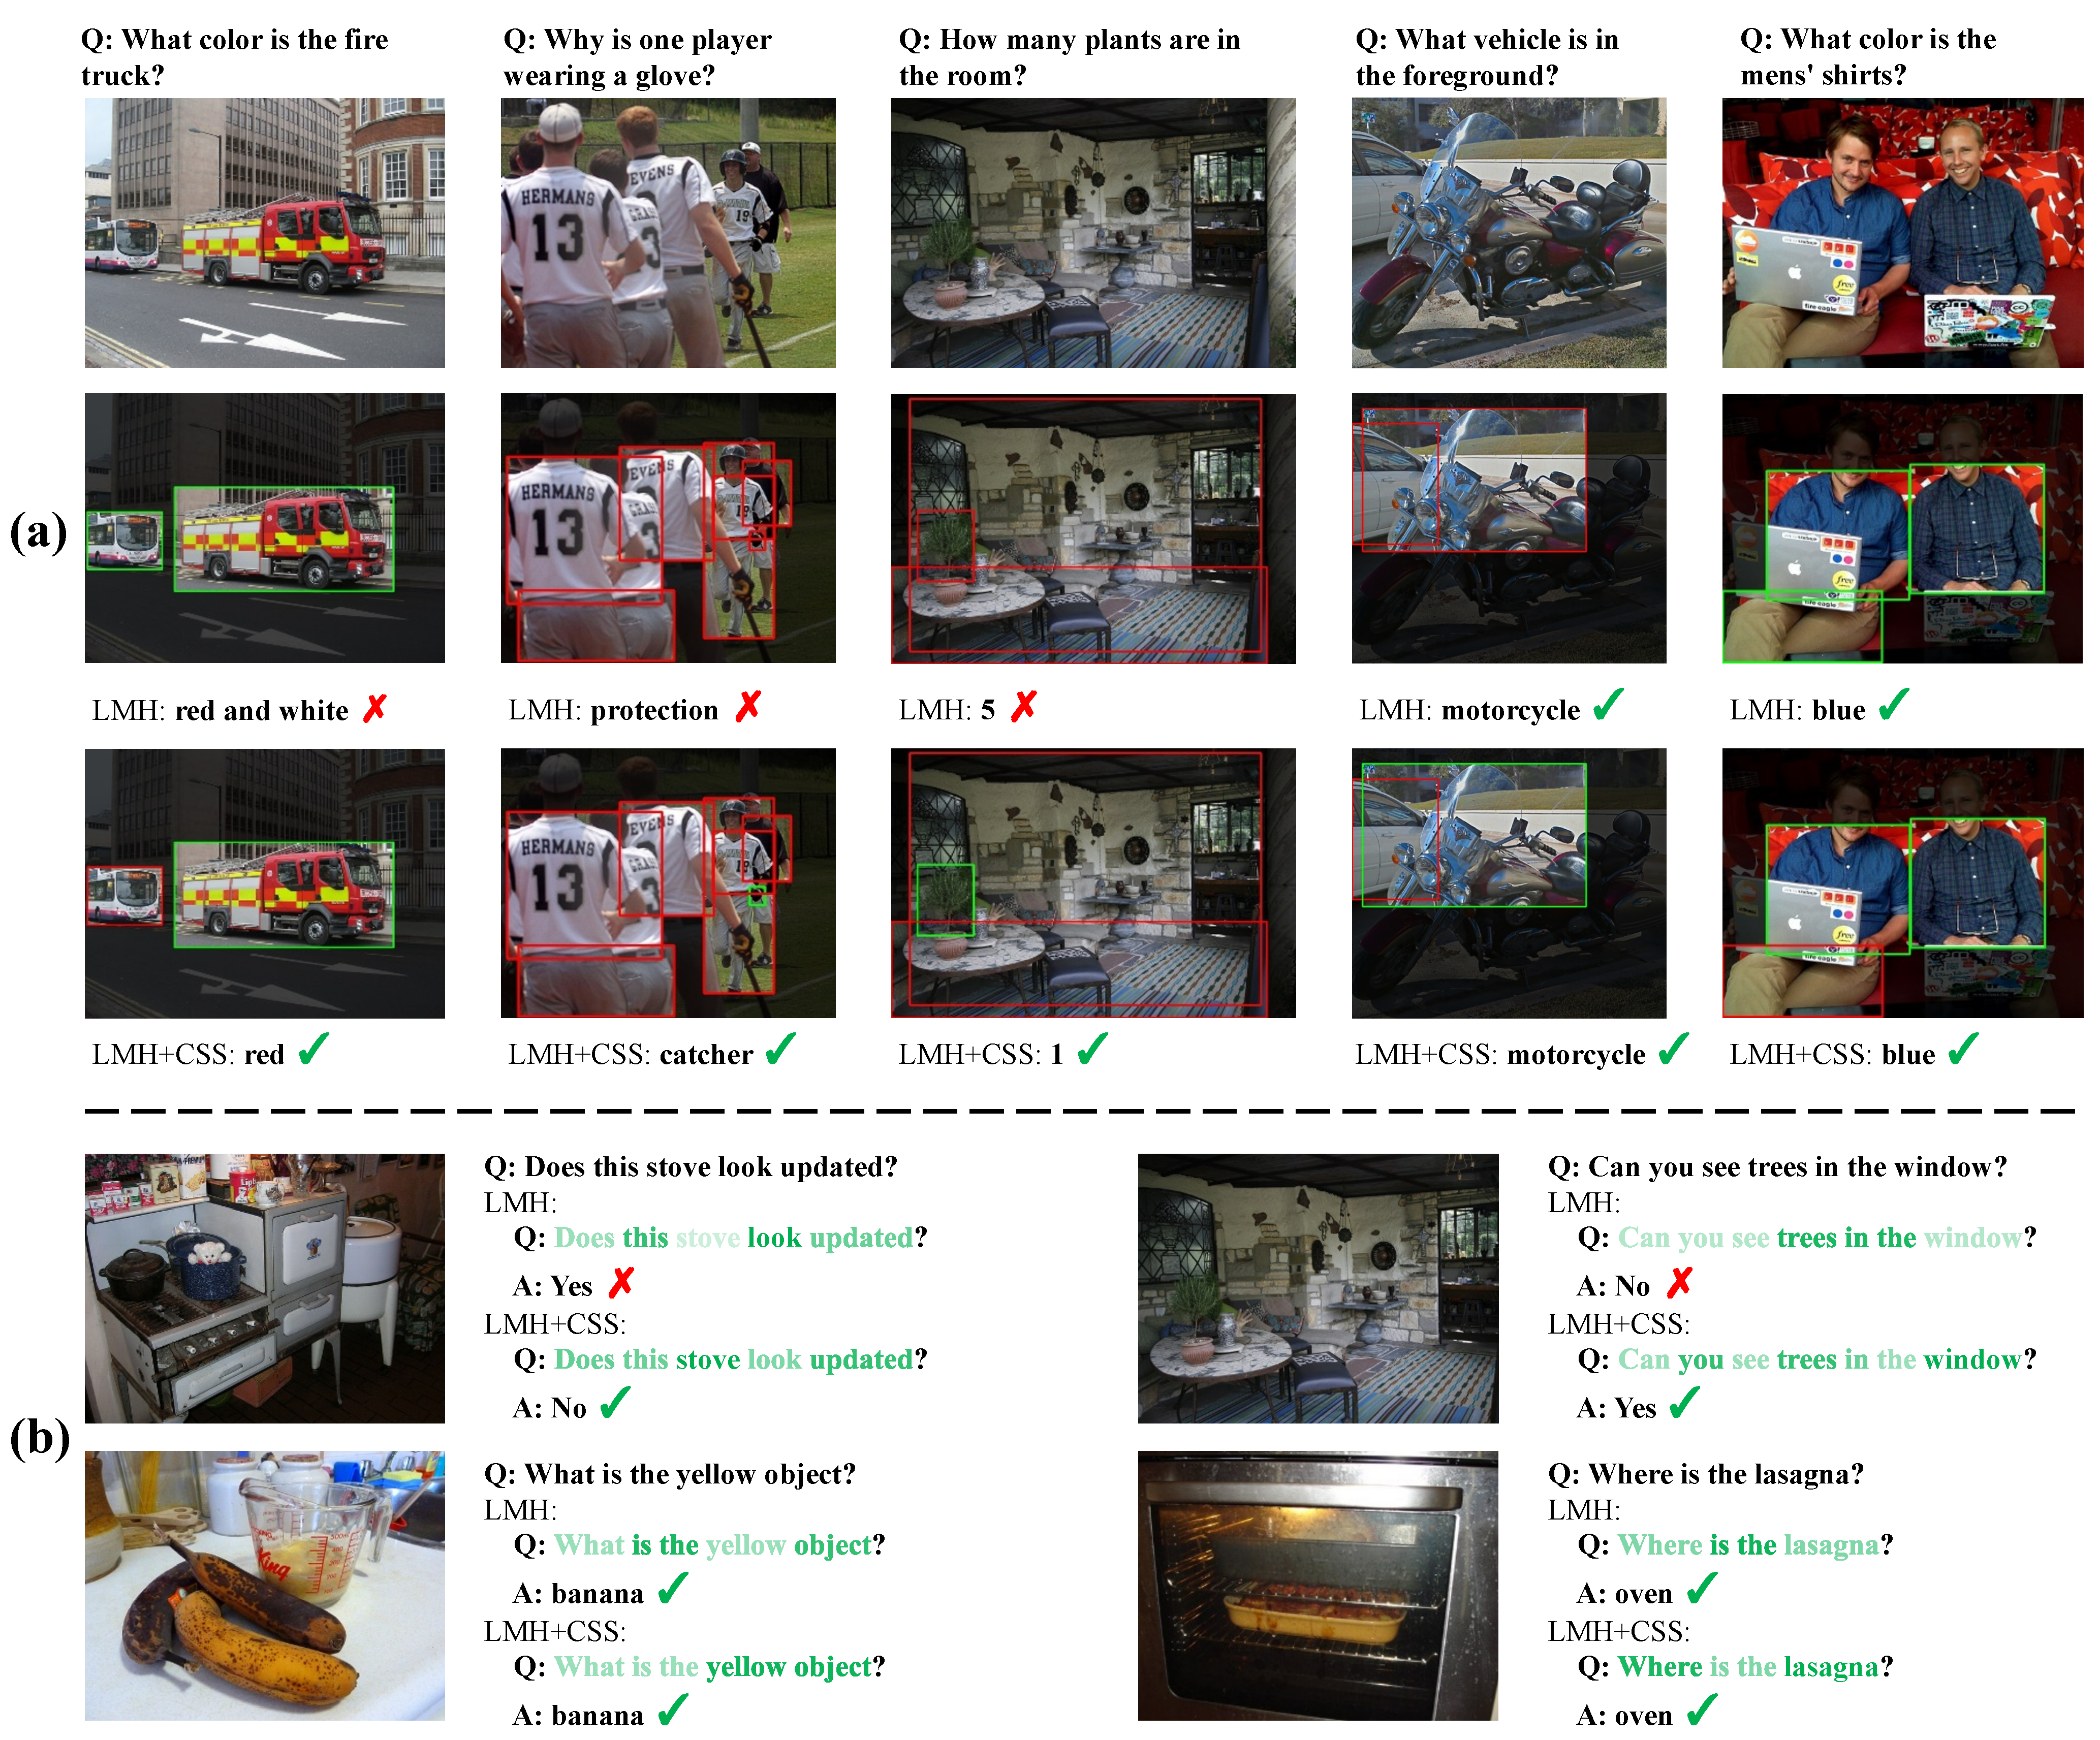
\includegraphics[width=0.95\linewidth]{chapter4/res/visualization.pdf}
    \caption{模型CMAT和模型MOTIFS在数据集Visual Genome上的场景图生成结果对比}
    \label{ch4:fig:visualization}
\end{figure}

\textbf{\kaishu{定性性能对比}}:图~\ref{ch4:fig:visualization}展示了模型CMAT和模型MOTIFS在数据集Visual Genome上的场景图生成结果。其中绿色框表示与真实物体框交叉比大于0.5的物体框,蓝色框表示模型的检测框但数据集中没有标注,红色框表示遗漏的真实物体框。绿色的边表示真阳性(true positive)的视觉关系预测,红色边表示假阴性(false negative)的视觉关系预测,以及蓝色边表示假阳性(false positive)的视觉关系预测。

由图~\ref{ch4:fig:visualization}前两排结果看出可以看出,模型CMAT很少遗漏一些重要的物体节点,如“laptop”、“surfboard”等。这主要原因是模型CMAT的优化目标满足整体一致性,往往对重要的物体节点赋予的权重更大。从第三排结果可以看出,模型CMAT的错误主要是检测出比模型MOTIFS更多的未标注的视觉关系(即蓝色边)。由于目前使用的评价指标主要是基于Recall@K,它只依据所有标注的视觉三元组的排序结果。因此,如果检测出更多的未标注的正样本,反而会得到更低的评价分数。


\section{本章小结}

在本章,我们提出图像场景图生成模型的优化目标应该同时具备整体一致性和局部敏感性。然而,现有的场景图生成模型基本都是使用所有物体和视觉关系分类的交叉熵之和作为模型的优化目标,缺乏整体一致性。为了解决这一问题,本章提出全新的反事实多智能体学习模型(CMAT)。模型CMAT首次将图像场景图生成任务转化成一个多智能体协同合作的决策问题,然后使用场景图生成的评价指标(如Recall@K)作为模型的优化目标,满足整体一致性要求。其次,模型CMAT中包含一个反事实基准模型,通过固定其他智能体的预测同时改变目标智能体的预测,来近似计算每个智能体的局部贡献,进而为每个智能体计算得到更加有效的训练信号。在大规模图像场景图生成数据集Visual Genome上的多个实验设定中,模型CMAT都可以通过提升物体类别的准确率,显著提升场景图生成质量。

\chapter{基于多层空间和通道注意力网络的图像描述生成方法}

注意力机制已经被广泛地运用在视觉场景理解任务中,如图像描述生成、视觉问答等。现有的注意力机制都是属于空间注意力机制,即只对卷积神经网络的最后一个特征图(feature map)在空间维度上进行加权。然而,卷积神经网络的特征图除了空间维度以外,还有通道和层级两个维度。因此,目前的注意力机制并没有充分利用卷积神经网络特征图的特性。在本章,我们提出一种全新的注意力机制网络:多层空间和通道注意力网络(Spatial and Channel-wise Attention in CNN, SCA-CNN)。对于图像描述生成任务,SCA-CNN在生成每个单词的过程中,动态地对不同层级下的特征图中所有的空间位置和通道进行加权,提升图像编码网络的表达能力。我们在图像描述生成的三个标准数据集(Flickr8K、Flickr30K、MSCOCO)对模型SCA-CNN进行评估,大量的对比实验结果都表明我们提出的多层空间和通道注意力网络(SCA-CNN)可以显著地提升图像描述生成质量。


\section{问题描述}

注意力机制已经被广泛地证明可以用来提升视觉场景理解任务的性能,如图像或视频的描述生成~\cite{xu2015show,yao2015describing}、视觉问答~\cite{chen2016abc,yang2016stacked,xu2016ask}等。在图像描述生成任务中,注意力机制的使用主要是基于一个合理的设想:人类在生成图像描述过程中,往往不是一次性直接记住整个图像,而是在生成语句的过程中不断地去调整关注的图像区域~\cite{corbetta2002control}。具体来说,与之前的图像描述生成工作直接将整个图像编码成一个固定的向量表达不同~\cite{vinyals2015show,karpathy2015deep},注意力机制让模型在语句生成的过程中不断地调整图像的特征表达,从而生成更加丰富和准确的描述语句。因此,注意力机制也可以被看成是一种动态的特征调节机制~\cite{mnih2014recurrent,stollenga2014deep}。

目前主要的图像视觉特征都是通过卷积神经网络进行编码~\cite{he2016deep,simonyan2015very}。给定一个大小为$W\times H\times 3$的彩色图像,通常卷积层用一个通道数为$C$的卷积核对输入图像进行卷积,得到一个大小为$W'\times H'\times C$的特征图,然后这个特征图又输入到后续的网络结构中。在三维的特征图中,每个通道本质上对应的是不同卷积核通道的响应。另一方面,卷积核也可以被看成是一种模式检测器:底层的卷积核往往倾向于检测一些底层的视觉特征(如:边、角等),而高层的卷积核往往倾向于检测一些高层的语义特征(如:物体等)~\cite{zeiler2014visualizing}。通过叠加多个卷积层,卷积神经网络实现对图像的多层语义特征提取。因此,卷积神经网络的图像特征本质上有三个维度:空间维度、通道维度、和层级维度。然而,目前所有注意力模型都只考虑了空间维度~\cite{xu2015show},即:只利用语句信息对卷积神经网络的最后一个特征图在空间维度上进行加权。

\begin{figure}[t]
    \centering
    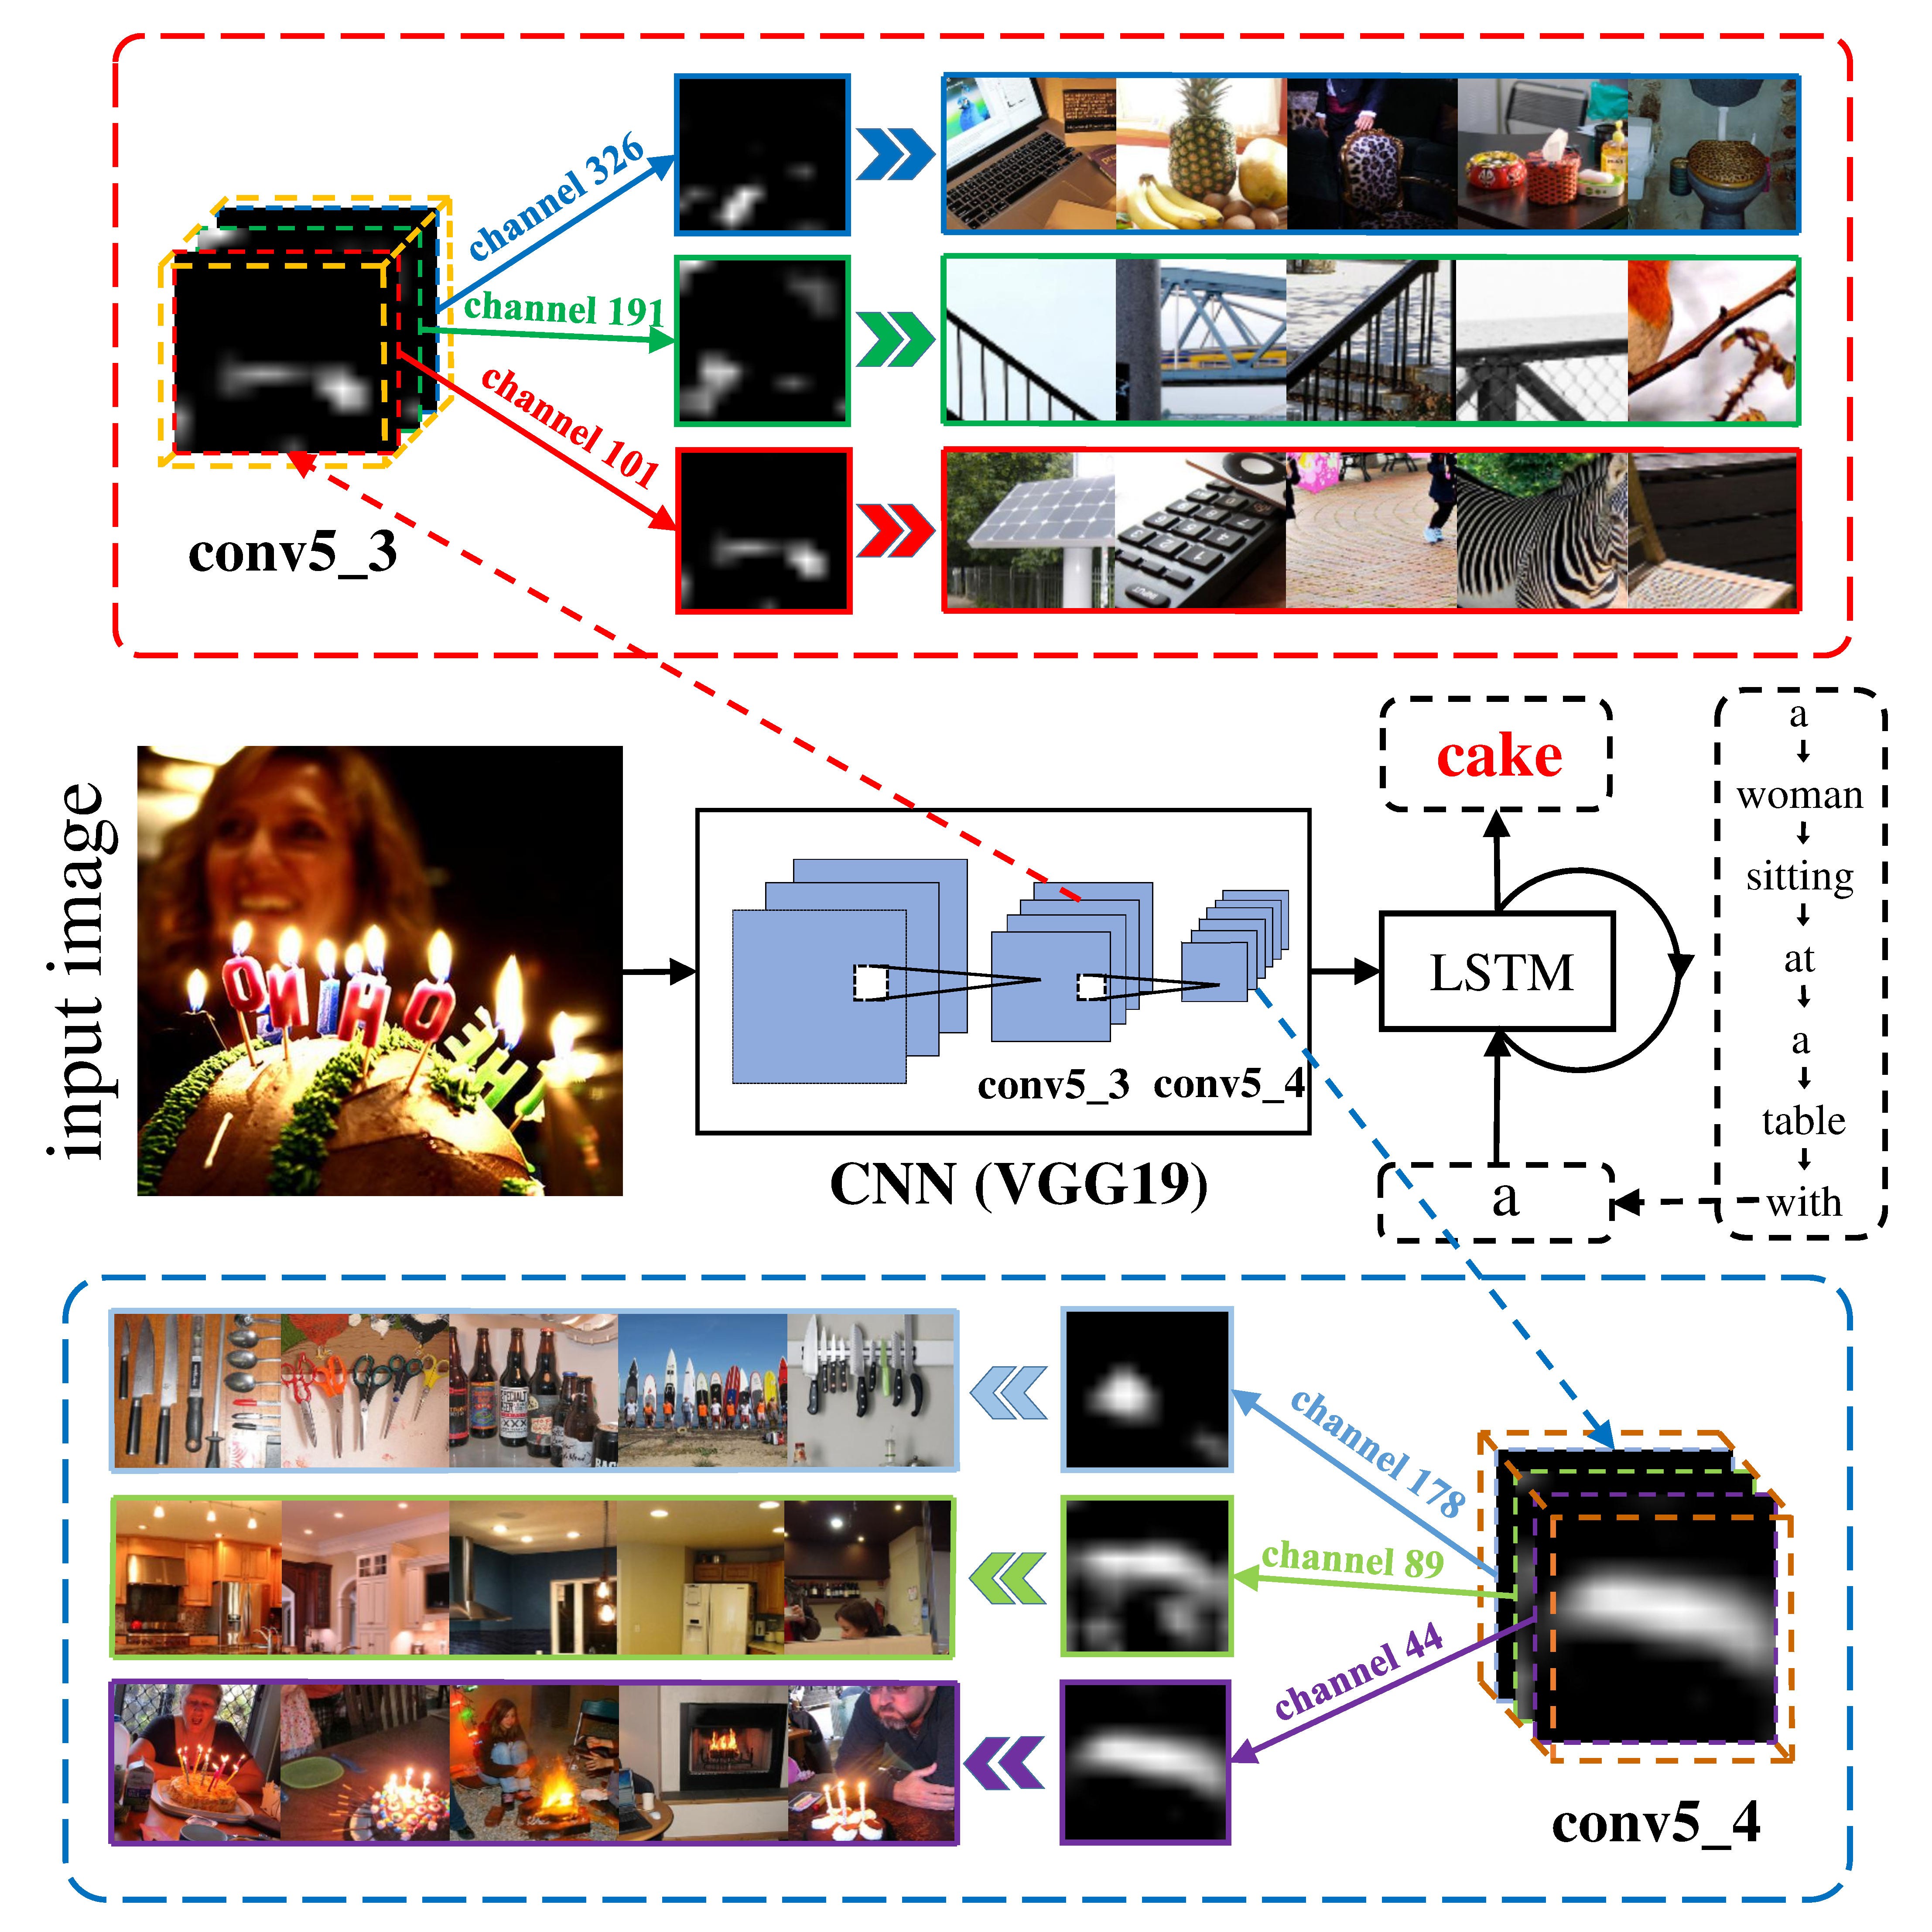
\includegraphics[width=0.9\linewidth]{chapter5/res/motivation.pdf}
    \caption{VGG19网络中conv5\_4层和conv5\_3层的通道注意力机制示意图}
    \label{ch5:fig:motivation}
\end{figure}

在本章,我们扩展现有的空间注意力模型,将注意力机制使用在卷积神经网络特征图的三个维度上。具体来说,我们提出了一种全新的网络结构:多层空间和通道注意力网络(SCA-CNN),对多个卷积层的所有元素都进行加权。如图~\ref{ch5:fig:motivation}所示,特征图的每一个通道本质上可以认为是一种特定属性或者物体检测器的响应结果,即通道注意力也可以看成是基于生成语句对不同的属性特征进行选择。例如,当模型要预测单词“cake”时,通道注意力机制(如图~\ref{ch5:fig:motivation}中的conv5\_4层和conv5\_3层)会对部分属性特征赋予更大的权重,如“火”、“光”、“蜡烛形状”等属性。另外,由于每个卷积层本质上都是底层卷积的输出结果,因此,可以对多个不同的卷积层同时在空间维度和通道维度使用注意力机制。例如,对于低层的特征图(如图~\ref{ch5:fig:motivation}中conv5\_3层)往往关注更加底层的属性特征。

我们在三个标准的图像描述生成数据集(Flickr8K、Flickr30K和MSCOCO)对模型SCA-CNN的性能进行评估。相比于现有的空间注意力模型~\cite{xu2015show},SCA-CNN可以在评价指标BLEU4上提升4.8\%。总而言之,我们提出了一种全新的注意力机制网络,对卷积神经网络特征层在空间上、通道上、和层级上三个维度使用注意力机制。SCA-CNN是一种通用的结构,可以运用在任意的卷积神经网络结构和网络层上,如VGG~\cite{simonyan2015very}、ResNet~\cite{he2016deep}等。SCA-CNN也帮助我们更好的理解卷积神经网络特征在描述语句生成过程中的变化过程。


\section{空间和通道注意力机制}

\subsection{概述}
我们采用流行的编码器-解码器框架(encoder-decoder framework)对图像生成描述语句,即先用编码器(如卷积神经网络)将图像编码成一个向量表达,然后再使用解码器(如递归神经网络)将图像编码向量解码成描述语句。如图~\ref{ch5:fig:architecture}所示,模型SCA-CNN利用语句信息对不同层级的特征图分别在空间维度和通道维度使用注意力机制。

假设当模型在生成第$t$个单词时,LSTM的隐含状态为$\bm{h}_{t-1}\in\mathbb{R}^d$,其中$d$是隐含状态的维度。对于第$l$层的特征,SCA-CNN根据$\bm{h}_{t-1}$和目前的卷积特征$\bm{V}^l$,可以得到新的卷积特征$\bm{X}^l$:
\begin{equation} \label{ch5:eq:eq_1}
\begin{split}
\bm{V}^l &= \textrm{CNN}\left(\bm{X}^{l-1}\right),\\
\gamma^l &= \Phi\left(\bm{h}_{t-1},\bm{V}^l\right),\\
\bm{X}^l &= f\left(\bm{V}^{l},\gamma^{l}\right).
\end{split}
\end{equation}
其中,$\Phi(\cdot)$是空间和通道注意力函数,$\bm{V}^l$是上一个卷积层的输出$\bm{X}^{l-1}$之后再接卷积层或池化层~\cite{simonyan2015very,he2016deep},$f(\cdot)$是线性加权函数。当卷积特征达到最后一层(第$L$层)时,我们使用$\bm{X}^L$来生成第$t$个单词:
\begin{equation}
\begin{split}
\bm{h}_t &= \textrm{LSTM}\left(\bm{h}_{t-1},\bm{X}^L,y_{t-1}\right),\\
y_t & \sim p_t = \textrm{softmax} \left(\bm{h}_t, y_{t-1} \right).
\end{split}
\end{equation}
其中,$p_t \in \mathbb{R}^{|\mathcal{D}|}$是字典中所有单词的预测概率,$\mathcal{D}$是预定义的字典,包含训练集所有语句中出现的所有单词。

当注意力参数$\gamma^l$与特征$\bm{V}^l$或$\bm{X}^l$具有相同的尺寸时(即$W^l\times H^l\times C^l$),网络的计算量大小为$\mathcal{O}(W^lH^lC^lk)$,其中$k$是将卷积网络特征$\bm{V}^l$和LSTM的隐含状态$\bm{h}_{t-1}$映射到同一空间中的维度大小。当特征图尺寸非常大时,对GPU的显存需求比较大。因此,我们提出将三维的$\gamma^l$分解成空间注意力参数$\alpha^l$和通道注意力参数$\beta^l$:
\begin{eqnarray}
\alpha^l &= & \Phi_s \left(\bm{h}_{t-1},\bm{V}^l\right),  \label{ch5:eq:eq_3} \\
\beta^l &= & \Phi_c \left(\bm{h}_{t-1},\bm{V}^l\right). \label{ch5:eq:eq_4}
\end{eqnarray}
其中$\Phi_c$和$\Phi_s$分别表示通道注意力模型和空间注意力模型。这种简化将极大地减小计算空间到$\mathcal{O}(C^lk+W^lH^lk)$。

\begin{figure}[tbp]
    \centering
    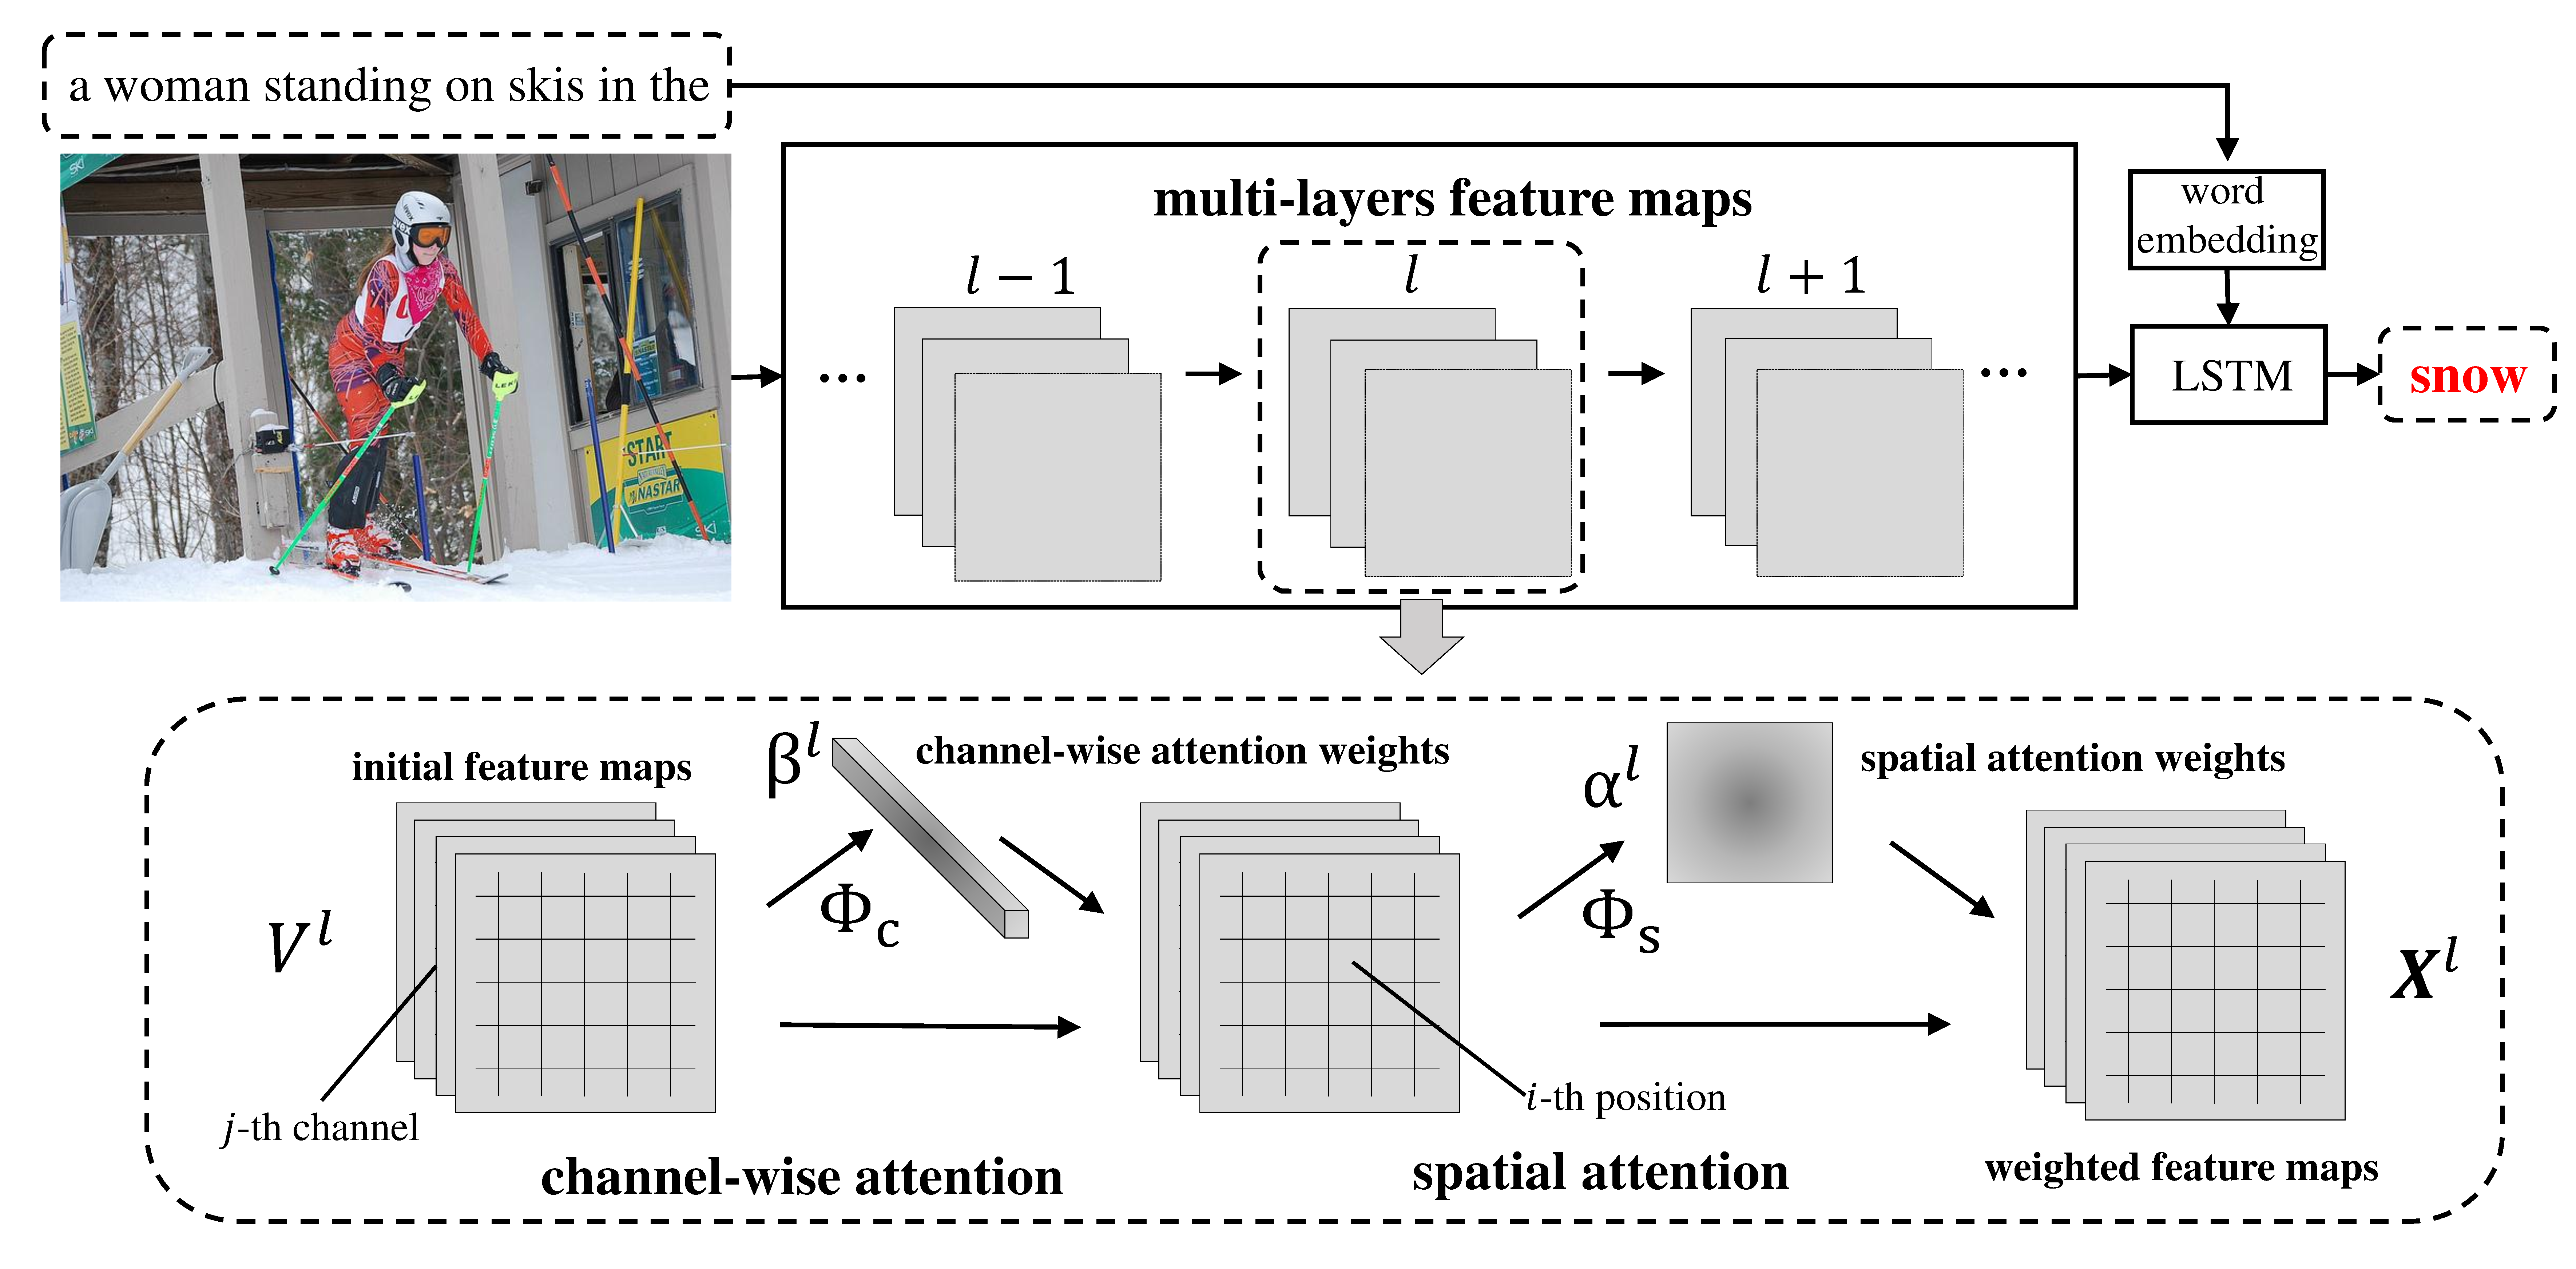
\includegraphics[width=\linewidth]{chapter5/res/architecture.pdf}
    \caption{空间和通道注意力卷积神经网络流程图}
    \label{ch5:fig:architecture}
\end{figure}

\subsection{空间注意力机制}
通常,语句中的每个单词只与图像中的部分区域有关,如图~\ref{ch5:fig:motivation}所示,当预测单词“cake”时,只有包含“蛋糕”的图像区域对于单词“cake”的预测有用。因此,在生成每个单词时,如果直接使用同一个全局图像特征,容易使模型陷入局部最优解。空间注意力机制就是对空间维度上不同的图像区域特征赋予不同的权重。为了不失一般性,我们省略层数上角标$l$。我们先将视觉特征$\bm{V}$改写成$\bm{V}  = \left[\bm{v}_1, \bm{v}_2, ..., \bm{v}_m
\right]$,其中$\bm{v}_i\in\mathbb{R}^C$,$m=W\cdot H$,$\bm{v}_i\in\mathbb{R}^C$可以看成是第$i$个位置的图像特征。给定上一个时刻的LSTM的隐含状态$\bm{h}_{t-1}$,我们使用单层神经网络来生成空间注意力权重$\alpha$:
\begin{equation} \label{ch5:eq:eq_5}
\begin{split}
\bm{a} & = \tanh \left( \left( \bm{W}_s \bm{V} + \bm{b}_s \right) \oplus \bm{W}_{hs}\bm{h}_{t-1}\right), \\
\alpha & = \textrm{softmax} \left( \bm{W}_i \bm{a} + b_i \right).
\end{split}
\end{equation}
其中,$\bm{W}_s \in \mathbb{R}^{k \times C}$、$\bm{W}_{hs} \in \mathbb{R}^{k \times d}$、$\bm{W}_i \in \mathbb{R}^k$都是需要学习的映射矩阵,其中$\bm{W}_s$和$\bm{W}_{hs}$分别将视觉特征、隐含状态映射到同一个维度。符号$\oplus$表示矩阵和向量之间相加,即对矩阵中的每一个列向量都加上该向量。$\bm{b}_s \in \mathbb{R}^k, b_i \in \mathbb{R}^1$是模型中可学习的偏置。


\subsection{通道注意力机制}
从公式~\ref{ch5:eq:eq_3}中可以看出,空间注意力机制需要使用视觉特征$\bm{V}$计算空间注意力参数,我们也同时可以使用通道注意力机制对$\bm{V}$在通道维度上进行加权。因为卷积神经网络的特征图的每一个通道本质上可以认为是一种特定属性或者物体检测器的响应结果,所以对特征图使用通道注意力机制可以看成是对不同的语义特征进行筛选的过程。

对于通道注意力机制,我们先将特征图$\bm{V}$改写成$\bm{U}$,其中$\bm{U} = [\bm{u}_1, \bm{u}_2, ..., \bm{u}_C]$,$\bm{u}_i \in \mathbb{R}^{W \times H}$表示特征图$\bm{V}$的第$i$个通道,$C$是总的通道数。然后,我们对每个通道使用平均池化,得到通道特征$\bm{v}$:
\begin{equation}
\bm{v} = \left[v_1, v_2, ..., v_C \right], \bm{v} \in \mathbb{R}^{C},
\end{equation}
其中标量$v_i$是向量$\bm{u}_i$的平均,表示第$i$个通道的特征。于是,通道注意力模型$\Phi_c$可以定义为:
\begin{equation} \label{ch5:eq:eq_7}
\begin{split}
\bm{b} & = \tanh \left(\left(\bm{W}_c \otimes \bm{v} + \bm{b}_c \right) \oplus \bm{W}_{hc}\bm{h}_{t-1} \right), \\
\beta & = \textrm{softmax} \left(\bm{W'}_i \bm{b} + {b'}_i \right).
\end{split}
\end{equation}
其中$\bm{W}_c \in \mathbb{R}^k$、$\bm{W}_{hc} \in \mathbb{R}^{k \times d}$和$\bm{W'}_i \in \mathbb{R}^k$是需要学习的映射矩阵,$\otimes$表示向量间的外积,$\bm{b}_c \in \mathbb{R}^k, {b'}_i \in \mathbb{R}^1$是模型可学习的偏置。


根据空间注意力模型和通道注意力模型的使用顺序,总共有两种不同的组合形式:

\textbf{\kaishu{通道-空间模型}}(Channel-Spatial):第一类是先使用通道注意力机制再使用空间注意力机制。对于这类,如图~\ref{ch5:fig:architecture}所示,给定一个初始的视觉特征图$\bm{V}$,我们先使用通道注意力模型$\Phi_c$得到通道注意力权重$\beta$,然后利用$\beta$对$\bm{V}$进行线性加权。之后,我们将加权的特征图输入到空间注意力模型$\Phi_s$得到空间注意力权重$\alpha$。在得到注意力权重$\alpha$和$\beta$之后,我们可以得到最终的特征图$\bm{X}$:
\begin{equation} \label{ch5:eq:eq_8}
\begin{split}
\beta &= \Phi_c \left(\bm{h}_{t-1},\bm{V} \right), \\
\alpha &= \Phi_s \left(\bm{h}_{t-1}, f_c \left(\bm{V}, \beta \right) \right), \\
\bm{X} &= f \left(\bm{V}, \alpha, \beta \right).
\end{split}
\end{equation}
其中,$f_c(\cdot)$表示特征图通道与通道注意力权重在通道维度上进行乘积。


\textbf{\kaishu{空间-通道模型}}(Spatial-Channel):第二类是先使用空间注意力机制再使用通道注意力机制。对于这类,给定一个初始的视觉特征图$\bm{V}$,我们先使用空间注意力模型$\Phi_s$得到空间注意力权重$\alpha$。通过注意力权重、线性函数$f_s(\cdot)$和通道注意力模型$\Phi_c$,我们可以得到最终的特征图$\bm{X}$:
\begin{equation} \label{ch5:eq:eq_9}
\begin{split}
\alpha &= \Phi_s \left(\bm{h}_{t-1}, \bm{V} \right), \\
\beta &= \Phi_c \left(\bm{h}_{t-1}, f_s \left(\bm{V}, \alpha \right) \right), \\
\bm{X} &= f \left(\bm{V}, \alpha, \beta \right).
\end{split}
\end{equation}
其中,$f_s(\cdot)$表示特征图空间不同区域特征与空间注意力权重进行乘积。


\section{实验设置与性能对比}
\subsection{图像描述生成任务的数据集和评价指标}

\textbf{\kaishu{图像描述生成数据集}}:我们在三个通用的图像描述生成数据集对模型SCA-CNN的性能进行评估。各个数据集具体的细节如下:

\textbf{Flickr8k}~\cite{hodosh2013framing}:它一共包含8000张图像。按照官方的数据集划分,其中6000张图像作为训练集,1000张图像为验证集,1000张图像为测试集。

\textbf{Flickr30k}~\cite{young2014image}: 它一共包含31000张图像。由于这个数据集缺少官方的数据集划分,我们参考Karpathy等人~\cite{karpathy2015deep}的数据集划分,将其中29000张图像作为训练集,1000张图像作为验证集,1000张图像作为测试集。

\textbf{MSCOCO}~\cite{lin2014microsoft}:根据该数据集的官方划分,训练集包含82783张图像,验证集包含40504张图像,以及测试集包含40775张图像。由于官方测试集中所有的图像都没有公开其中的人工标注信息。我们同样参考Karpathy等人~\cite{karpathy2015deep}的数据集划分,其中验证集和测试集各包含5000张图像。

\textbf{\kaishu{图像描述生成评价指标}}:我们在四个常用的图像描述生成评价指标对模型SCA-CNN的性能进行评估。各个评价指标具体的细节如下:

\textbf{BLEU}~\cite{papineni2002bleu} (B@1, B@2, B@3, B@4):BLEU(Bilingual evaluation understudy)通过比较生成语句和所有人工标注语句中的n元词组(n-gram)的准确率,然后对所有的n元词组准确率计算几何平均数。其中,四元词组(即$n=4$)时计算得到的评估结果与人工的评估结果最接近。

\textbf{METEOR}~\cite{banerjee2005meteor} (MT):METEOR(Metric for Evaluation of Translation with Explicit ORdering)是基于生成语句和人工标注语句中一元词组的对齐关系。先对所有的一元词组进行精确匹配、近义词匹配、词干匹配之后,计算所有一元词组匹配的F分数(F-measure)。同时,METEOR引入一个权重系数,对生成过长的语句减小权重系数,通过对F分数进行加权得到每个生成语句的分数。对于多个人工标注语句,METEOR分别用生成语句和每个标注语句单独计算分数,然后选取其中的最高分作为最终的分数。

\textbf{CIDEr}~\cite{vedantam2015cider} (CD):CIDEr(Consensus-based Image Description Evaluation)先将所有单词进行词干提取(stemming),然后对所有预处理后的语句中的n元词组利用TF-IDF~\cite{robertson2004understanding}进行加权,
最后利用所有n元词组的余弦相似度得到分数。

\textbf{ROUGE-L}~\cite{lin2002manual} (RG):ROUGE(Recall-Oriented Understudy for Gisting Evaluation)先找到生成语句和人工标注语句之间最长的相同序列,然后基于最长的相同序列计算匹配的F分数。同样,对于多个人工标注语句,ROUGE-L分别单独计算与每个标注语句的分数,然后选取最高分作为最终分数。

总之,这四种评价指标都是通过比较生成语句和人工标注语句中n元词组的匹配程度。所有实验中这些评价指标的计算都是直接采用MSCOCO官方的测评工具:https://github/tylin/coco-caption。


\subsection{实验细节设定}
对于图像编码部分,我们采用两种流行的卷积神经网络:VGG-19~\cite{simonyan2015very}和ResNet-152~\cite{he2016deep}。对于文本解码部分,我们使用递归神经网络LSTM~\cite{hochreiter1997long}来生成描述语句。单词编码向量的维度和LSTM的隐含状态的维度分别设定为100和1000。用于计算注意力权重的共同空间维度设置为512。对于Flickr8k数据集,批处理大小设置为16;对于Flickr30k和MSCOCO,批处理大小设置为64。为了避免模型过拟合,我们采用dropout和early stopping机制。整个SCA-CNN模型直接采用端到端的训练方式,用优化算法Adadelta~\cite{zeiler2012adadelta}进行参数优化。当模型刚好预测一个特定的“END”字符或者达到了预先设定的句子最长的长度时,整个语句的生成过程将会终止。在测试阶段,我们采用BeamSearch~\cite{vinyals2015show}的方法,在每个时刻选择5个语句作为候选答案。


\subsection{通道注意力机制的性能分析}

\textbf{\kaishu{实验设定}}:本小节主要探讨通道注意力机制对现有空间注意力模型的影响。我们总共比较了五种实验设定:(1)\textbf{Spatial}:它是一个空间注意力模型,对卷积网络最后一层特征图先计算空间注意力权重,然后对最后一层特征图的不同空间区域特征进行加权。对于VGG19和ResNet152网络,最后一层分别为conv5\_4和res5c。在对最后一层特征图进行加权之后,我们将加权后的特征图输入的原本的网络结构中。对于VGG19网络而言,conv5\_4层之后还有两个全连接层;对于ResNet152网络而言,res5c层之后是一个平均池化层。(2)\textbf{Channel}:它是一个通道注意力模型,和空间注意力模型Spatial基本相同,除了将空间注意力模型(公式~\eqref{ch5:eq:eq_3})替换成通道注意力模型(公式~\eqref{ch5:eq:eq_4})。(3)\textbf{Channel-Spatial}:第一种融合方式,先使用通道注意力模型,再使用空间注意力模型(公式~\eqref{ch5:eq:eq_8})。(4)\textbf{Spatial-Channel}:第二种融合方式,先使用空间注意力模型,再使用通道注意力模型(公式~\eqref{ch5:eq:eq_9})。(5)\textbf{HAT}:它是Xu等人~\cite{xu2015show}提出的“硬注意力”模型(Hard-ATtention, HAT)。HAT模型和Spatial模型一样,都属于空间注意力模型。但是与Spatial模型主要有两个区别:第一个是注意力权重和特征图的融合方式,第二个是是否将加权的特征图输入到后续的网络结构中。所有的实验结果都展示在表~\ref{ch5:tab:Q1}中。

%%%%%%%%%%%%%%%%%%%%%% Q1 %%%%%%%%%%%%%%%%%%%%%%%%%%%%%%%
\begin{table}[t]
\centering
\scalebox{0.9}{
\begin{tabular}{|l| l |l| c c c c|}
\hline
 Dataset & Network &Method & B@4 & MT & RG & CD\\
\hline
\multirow{10}{*}{Flickr8k} & \multirow{5}{*}{VGG} & Spatial & 23.0 & 21.0 & 49.1 & \textbf{60.6} \\
&  & HAT & 21.3 & 20.3 & --- & --- \\
&  & Channel & 22.6 & 20.3 & 48.7 & 58.7 \\
& & Spatial-Channel &22.6 & 20.9 & 48.7 & \textbf{60.6}\\
& & Channel-Spatial & \textbf{23.5} & \textbf{21.1} & \textbf{49.2} & 60.3\\
\cline{2-7}
& \multirow{5}{*}{ResNet} & Spatial & 20.5 & 19.6 & 47.4 & 49.9 \\
&  & HAT & 21.7 & 20.1 & 48.4 & 55.5 \\
&  & Channel & 24.4 & 21.5 & 50.0 & 65.5 \\
& & Spatial-Channel &24.8 & \textbf{22.2} & 50.5& 65.1\\
& & Channel-Spatial & \textbf{25.7} & 22.1& \textbf{50.9} & \textbf{66.5}\\
\hline
\multirow{10}{*}{Flickr30k} & \multirow{5}{*}{VGG} & Spatial & \textbf{21.1} & 18.4 & 43.1 & \textbf{39.5} \\
&  & HAT & 19.9 & \textbf{18.5} &  --- & --- \\
&  & Channel & 20.1 & 18.0 & 42.7 & 38.0 \\
& & Spatial-Channel & 20.8 & 17.8&42.9 & 38.2\\
& & Channel-Spatial & 21.0 & 18.0& \textbf{43.3} & 38.5\\
\cline{2-7}
& \multirow{5}{*}{ResNet} & Spatial & 20.5 & 17.4 & 42.8 & 35.3 \\
&  & HAT & 20.1 & 17.8 & 42.9 & 36.3 \\
&  & Channel & 21.5 & 18.4 & 43.8 & 42.2 \\
& & Spatial-Channel &21.9 & 18.5 & 44.0& \textbf{43.1}\\
& & Channel-Spatial & \textbf{22.1} & \textbf{19.0} & \textbf{44.6} & 42.5 \\
\hline
\multirow{10}{*}{MS COCO} & \multirow{5}{*}{VGG} & Spatial & \textbf{28.2} & 23.3 & \textbf{51.0} & \textbf{85.7} \\
&  & HAT & 25.0 & 23.0 & --- & --- \\
&  & Channel & 27.3 & 22.7 & 50.1 & 83.4 \\
& & Spatial-Channel &28.0 &23.0 & 50.6& 84.9\\
& & Channel-Spatial & 28.1 & \textbf{23.5} & 50.9& 84.7\\
\cline{2-7}
& \multirow{5}{*}{ResNet} & Spatial & 28.3 & 23.1 & 51.2 & 84.0 \\
&  & HAT & 28.4 & 23.2 & 51.2 & 84.9 \\
&  & Channel & 29.5 & 23.7 & 51.8 & 91.0 \\
& & Spatial-Channel &29.8 &23.9 & 52.0& 91.2\\
& & Channel-Spatial & \textbf{30.4} & \textbf{24.5} & \textbf{52.5} & \textbf{91.7}\\
\hline
\end{tabular}}
\caption{VGG-19网络和ResNet-152网络中单层注意力机制的性能对比} 
\label{ch5:tab:Q1}
\end{table}
%%%%%%%%%%%%%%%%%%%%%%%%%%%%%%%%%%%%%%%%%%%%%%%%%%%%%%%%%

\textbf{\kaishu{实验结果}}:从表~\ref{ch5:tab:Q1}中可以得到以下发现:(1)对于VGG19网络而言,Spatail模型的结果比HAT的好;但对于ResNet152网络,实验结果相反。这主要的原因在于VGG19网络中有全连接层,可以保持空间语义信息,而ResNet152网络中只有平均池化层,将会破坏原有的空间语义信息。(2)相比于VGG19网络,Channel模型在ResNet152网络中可以显著提升性能(与Spatial模型相比)。这主要的原因在于ResNet152网络的最后一个卷积特征图拥有更多的通道数(如:ResNet152有2048个通道,而VGG19网络只有512个通道)。(3)在ResNet152网络中,相比于Spatial模型,Channel-Spatial和Spatial-Channel都能显著提升性能。这说明通道注意力机制在特征图通道数足够大时能显著提升性能。(4)在VGG19网络和ResNet152网络中,Channel-Spatial和Spaital-Channel两个模型的效果都非常接近,其中Channel-Spatial稍微高一点。在之后的实验中,我们使用Channel-Spatial作为空间注意力机制和通道注意力机制的融合方式。


%%%%%%%%%%%%%%%%%%%%%% Q2_1 %%%%%%%%%%%%%%%%%%%%%%%%%%
\begin{table}[t]
\centering
\scalebox{0.9}{
\begin{tabular}{|l| l |l| c c c c|}
\hline
 Dataset & Network &Method & B@4 & MT & RG & CD\\
\hline
\multirow{6}{*}{Flickr8k} & \multirow{3}{*}{VGG} & 1-layer & \textbf{23.0} & 21.0 & \textbf{49.1} & \textbf{60.6} \\
&  & 2-layer & 22.8 & \textbf{21.2} & 49.0 & 60.4 \\
&  & 3-layer & 21.6 & 20.9 & 48.4 & 54.5 \\
\cline{2-7}
& \multirow{3}{*}{ResNet} & 1-layer & 20.5 & 19.6 & 47.4 & 49.9 \\
&  & 2-layer & 22.9 & 21.2 & 48.8 & 58.8 \\
&  & 3-layer & \textbf{23.9} & \textbf{21.3} & \textbf{49.7} & \textbf{61.7} \\
\hline
\multirow{6}{*}{Flickr30k} & \multirow{3}{*}{VGG} & 1-layer & 21.1 & 18.4 & 43.1 & \textbf{39.5} \\
&  & 2-layer & \textbf{21.9} & \textbf{18.5} & \textbf{44.3} & \textbf{39.5} \\
&  & 3-layer & 20.8 & 18.0 & 43.0 & 38.5 \\  %%%%%%%%%
\cline{2-7}
& \multirow{3}{*}{ResNet} & 1-layer & 20.5 & 17.4 & 42.8 & 35.3 \\
&  & 2-layer & 20.6 & 18.6 & 43.2 & 39.7 \\
&  & 3-layer & \textbf{21.0} & \textbf{19.2} & \textbf{43.4} & \textbf{43.5} \\
\hline
\multirow{6}{*}{MS COCO} & \multirow{3}{*}{VGG} & 1-layer & 28.2 & 23.3 & 51.0 & 85.7 \\
&  & 2-layer & \textbf{29.0} & \textbf{23.6} & \textbf{51.4} & \textbf{87.4}\\
&  & 3-layer & 27.4 & 22.9 & 50.4 & 80.8 \\
\cline{2-7}
& \multirow{3}{*}{ResNet} & 1-layer & 28.3 & 23.1 & 51.2 & 84.0 \\
&  & 2-layer & \textbf{29.7} & 24.1 & \textbf{52.2} & \textbf{91.1} \\
&  & 3-layer & 29.6 & \textbf{24.2} & 52.1 & 90.3 \\
\hline
\end{tabular}}
\caption{空间注意力模型在VGG-19网络和ResNet-152网络下不同层的性能对比} 
\label{ch5:tab:Q2_1}
\end{table}
%%%%%%%%%%%%%%%%%%%%%%%%%%%%%%%%%%%%%%%%%%%%%%%%%%%%%


\subsection{多层注意力机制的性能分析}

\textbf{\kaishu{实验设定}}:本小节主要探讨在卷积神经网络的不同层级中使用空间注意力机制或通道注意力机制对模型性能的影响。我们分别对Spatial模型和Channel-Spatial模型进行了不同层级的实验:“一层”(1-layer)、“两层”(2-layer)、“三层”(3-layer)分别表示在一个层级、两个层级和三个层级上使用注意力机制。对于VGG19网络,这三个层级分别表示:conv5\_4、conv5\_3和conv5\_2;对于ResNet152网络,这三个层级分别表示res5c、res5c\_branch2b和res5c\_branch2a。

%%%%%%%%%%%%%%%%%%%%% Q2_2 %%%%%%%%%%%%%%%%%%%%%%%%%
\begin{table}[t]
\centering
\scalebox{0.9}{
\begin{tabular}{|l| l |l| c c c c|}
\hline
 Dataset & Network &Method & B@4 & MT & RG & CD\\
\hline
\multirow{6}{*}{Flickr8k} & \multirow{3}{*}{VGG} & 1-layer & \textbf{23.5} & 21.1 & 49.2 & 60.3 \\
&  & 2-layers & 22.8 & \textbf{21.6} & \textbf{49.5} & 62.1 \\
&  & 3-layers & 22.7 & 21.3 & 49.3 & \textbf{62.3} \\
\cline{2-7}
& \multirow{3}{*}{ResNet} & 1-layer & 25.7 & 22.1 & 50.9 & 66.5 \\
&  & 2-layers & \textbf{25.8} & 22.4 & \textbf{51.3} & 67.1 \\
&  & 3-layers & 25.3 & \textbf{22.9} & 51.2 & \textbf{67.5} \\
\hline
\multirow{6}{*}{Flickr30k} & \multirow{3}{*}{VGG} & 1-layer & 21.0 & 18.0 & 43.3 & 38.5 \\
&  & 2-layers & \textbf{21.8} & \textbf{18.8} & \textbf{43.7} & \textbf{41.4} \\
&  & 3-layers & 20.7 & 18.3 & 43.6 & 39.2 \\
\cline{2-7}
& \multirow{3}{*}{ResNet} & 1-layer & 22.1 & 19.0 & 44.6 & 42.5 \\
&  & 2-layers & \textbf{22.3} & \textbf{19.5} & \textbf{44.9} & \textbf{44.7} \\
&  & 3-layers & 22.0 & 19.2 & 44.7 & 42.8 \\        %%
\hline
\multirow{6}{*}{MS COCO} & \multirow{3}{*}{VGG} & 1-layer & 28.1 & 23.5 & 50.9 & 84.7 \\
&  & 2-layers & \textbf{29.8} & \textbf{24.2} & \textbf{51.9} & \textbf{89.7} \\
&  & 3-layers & 29.4 & 24.0 & 51.7 & 88.4 \\    %%
\cline{2-7}
& \multirow{3}{*}{ResNet} & 1-layer & 30.4 & 24.5 & 52.5 & 91.7 \\
&  & 2-layers & \textbf{31.1} & \textbf{25.0} & \textbf{53.1} & \textbf{95.2} \\
&  & 3-layers & 30.9 & 24.8 & 53.0 & 94.7 \\   %%
\hline
\end{tabular}}
\caption{空间和通道注意力模型在VGG-19网络和ResNet-152网络下不同层的性能对比} 
\label{ch5:tab:Q2_2}
\end{table}
%%%%%%%%%%%%%%%%%%%%%%%%%%%%%%%%%%%%%%%%%%%%%%%%%%%%%%%%%

\textbf{\kaishu{实验结果}}:从表~\ref{ch5:tab:Q2_1}的结果和表~\ref{ch5:tab:Q2_2}结果,我们有以下发现:(1)在绝大多数的实验设定中,模型都可以通过在更多的卷积层上使用注意力机制来提升实验结果。这主要是因为在多层特征上使用注意力机制可以帮助模型对不同层次的语义特征上进行选择性关注。(2)在太多的卷积层上使用注意力机制也容易造成过拟合。例如:当注意力机制改变的层数增加时,Flickr8K更容易造成性能下降。这主要原因是因为Fickr8K有6000张训练图像,而MSCOCO有82783张训练图像。


\subsection{空间和通道注意力卷积神经网络的性能比较}

\textbf{\kaishu{实验设定}}:我们将本章提出的模型SCA-CNN与目前最好的图像描述生成方法进行对比,这些方法主要可以分为三类:(1)\textbf{Deep VS}~\cite{karpathy2015deep}、\textbf{NIC}~\cite{vinyals2015show}、\textbf{m-RNN}~\cite{mao2015deep}。这些方法都是端到端的编码-解码框架,并且模型中没有包含注意力机制。(2)\textbf{SAT}~\cite{xu2015show}和\textbf{HAT}~\cite{xu2015show}是空间注意力模型。其中模型SAT(Soft-ATtention)是在每步生成单词的过程中对所有的空间区域进行线性加权,而模型HAT(Hard-ATtention)是在每步生成单词的过程中对所有的区域只采样其中一个区域特征。(3)\textbf{gLSTM}~\cite{jia2015guiding}和\textbf{ATT}~\cite{you2016image}是属性注意力模型。其中模型gLSTM使用图像和生成的描述语句作为全局的属性信息,而模型ATT使用图像额外检测的属性作为属性信息。表~\ref{ch5:tab:sota}的结果“ours(V)”和“ours(R)”分别表示VGG19网络和ResNet152网络中两层Channel-Spatial模型。另外,我们还将模型上传到MSCOCO在线服务器对官方测试集进行预测,结果展示在表~\ref{ch5:tab:server}中。

\begin{figure}[t]
    \centering
    \includegraphics[width=\linewidth]{chapter5/res/visualization.pdf}
    \caption{空间注意力和通道注意力权重的可视化结果}
    \label{ch5:fig:visualization}
\end{figure}

%%%%%%%%%%%%%%%%%%%%%%% Q3 %%%%%%%%%%%%%%%%%%%%%%%%%%%
\begin{table*}[t]
\centering
\scalebox{0.85}{
\begin{tabular}{ |l | c c c c  | c c c c | c c c c|}
\hline
\multirow{2}{*}{Model} & \multicolumn{4}{c|}{Flickr8k} & \multicolumn{4}{c|}{Flickr30k} & \multicolumn{4}{c|}{MS COCO} \\
\cline{2-13}
& B@2 & B@3 & B@4 & MT & B@2 & B@3 & B@4 & MT & B@2 & B@3 & B@4 & MT \\
\hline
Deep VS & 38.3 & 24.5 & 16.0 & -- &  36.9 & 24.0 & 15.7 & --  & 45.0 & 32.1 & 23.0 & 19.5 \\
NIC & 41.0 & 27.0 & -- & -- & 42.3 & 27.7 & 18.3  & -- & 46.1 & 32.9 & 24.6 & -- \\
m-RNN & -- & -- & -- & -- & 41.0 & 28.0 & 19.0 & -- & 49.0 & 35.0 & 25.0 & -- \\
SAT & 44.8 & 29.9 & 19.5 & 18.9 & 43.4 & 28.8 & 19.1 & 18.5 & 49.2 & 34.4 & 24.3 & 23.9 \\
HAT & 45.7 & 31.4 & 21.3 & 20.3 & 43.9 & 29.6 & 19.9 & 18.5 & 50.4 & 35.7 & 25.0 & 23.0 \\
gLSTM & 45.9 & 31.8 & 21.2 & 20.6 & 44.6 & 30.5 & 20.6 & 17.9 & 49.1 & 35.8 & 26.4 & 22.7 \\
ATT & -- & -- & -- & --  & 46.0 & 32.4 & \textbf{23.0} & 18.9 & 53.7 & 40.2 & 30.4 & 24.3  \\
\hline
ours(V) & 46.6 & 32.6 & 22.8 & 21.6 & 45.3 & 31.7 & 21.8 & 18.8 & 53.3 & 39.7 & 29.8 & 24.2\\
ours(R)  & \textbf{49.6} & \textbf{35.9} & \textbf{25.8} & \textbf{22.4} & \textbf{46.8} & \textbf{32.5} & 22.3 & \textbf{19.5} & \textbf{54.8} & \textbf{41.1} & \textbf{31.1} & \textbf{25.0}\\
\hline
\end{tabular}}
\caption{不同描述语句生成算法在数据集Flickr8k、Flickr30k和MSCOCO上的性能对比} 
\label{ch5:tab:sota}
\end{table*}
%%%%%%%%%%%%%%%%%%%%%%%%%%%%%%%%%%%%%%%%%%%%%%%%%%%%%%%%%

%%%%%%%%%%%%%%%%%%%%%%% sever %%%%%%%%%%%%%%%%%%%%%%%
\begin{table*}[t]
\centering
\scalebox{0.8}{
\begin{tabular}{ |l | c | c | c| c | c |c | c |c | c |c | c| c | c |c | }
\hline
\multirow{2}{*}{Model} & \multicolumn{2}{c|}{B@1} & \multicolumn{2}{c|}{B@2} & \multicolumn{2}{c|}{B@3} & \multicolumn{2}{c|}{B@4} &\multicolumn{2}{c|}{METEOR} & \multicolumn{2}{c|}{ROUGE-L} & \multicolumn{2}{c|}{CIDEr} \\
\cline{2-15}
& c5 & c40 & c5 & c40 & c5 & c40 & c5 & c40 & c5 & c40 & c5 & c40 & c5 & c40 \\
\hline
ours & 71.2 & 89.4 & 54.2& 80.2& 40.4& 69.1& 30.2& 57.9& 24.4 & 33.1 & 52.4 & 67.4& 91.2 & 92.1 \\
\hline
HAT  & 70.5& 88.1& 52.8& 77.9& 38.3 & 65.8 & 27.7 & 53.7 & 24.1 & 32.2& 51.6 &65.4 & 86.5 & 89.3\\
\hline
ATT & \textbf{73.1} & \textbf{90.0} & \textbf{56.5} & \textbf{81.5} & \textbf{42.4} & \textbf{70.9} & \textbf{31.6} & \textbf{59.9} &25.0 & \textbf{33.5} & 53.5& \textbf{68.2} & \textbf{95.3} & \textbf{95.8}   \\
\hline
NIC & 71.3 & 89.5 & 54.2& 80.2& 40.7& 69.4& 30.9& 58.7 & \textbf{25.4} & \textbf{34.6} & 53.0 & \textbf{68.2} & 94.3 & 94.6 \\
\hline
\end{tabular}}
\caption{不同图像描述语句生成算法在数据集MSCOCO的在线服务器上的性能对比} 
\label{ch5:tab:server}
\end{table*}
%%%%%%%%%%%%%%%%%%%%%%%%%%%%%%%%%%%%%%%%%%%%%%%%%%%%

\textbf{\kaishu{实验结果}}:从表~\ref{ch5:tab:sota}和表~\ref{ch5:tab:server}中可以看出,模型SCA-CNN可以超过目前现有的模型,这是因为SCA-CNN分别考虑了卷积神经网络特征层的三个维度:空间、通道和层级,而其他的方法只考虑了其中一个维度。在MSCOCO在线服务器上,模型SCA-CNN性能比模型ATT和模型NIC低的主要原因来自两个方面:(1)ATT和NIC的结果都是基于集成模型(ensemble model)的结果,而SCA-CNN是单个模型的结果。(2)它们使用更强的卷积神经网络对输入图像提取特征,如模型NIC使用Inception-V3网络~\cite{szegedy2016rethinking}而SCA-CNN只使用ResNet152网络。


\subsection{空间注意力和通道注意力权重的可视化}
如图~\ref{ch5:fig:visualization}所示,我们还提供了模型SCA-CNN的注意力权重在VGG19网络的可视化示例。其中“Layer-1”和“Layer-2”分别表示conv5\_4和conv5\_3层。每个示例包含三句描述语句:“Ours”(SCA-CNN)、“SAT”(Soft-ATtention)和“GT”(Ground Truth)。第二列的上部分是空间注意力权重,白色部分表示空间注意力权重较大,而灰色部分表示空间注意力权重较小。第二列下部分为所有通道权重的直方统计图。第三列的数字表示通道注意力权重最大的两个通道编号。后面的五张图像是数据集MSCOCO训练集中对同样通道编号响应最大的图像。为了简洁,我们只展示了预测语句中的其中一步。例如第一个例子,当模型SCA-CNN准备预测单词“umbrella”时,我们的通道注意力机制往往对例如“伞”、“棍状”以及“圆形”等语义信息响应强烈的通道赋予更大的权重。为了表示每个通道表示的语义信息,我们使用和Zeiler等人~\cite{zeiler2014visualizing}相同的方法,其中红色框表示对应通道最强响应的感受野。


\section{本章小结}

在本章,我们提出了一种全新的基于注意力机制的卷积神经网络:多层空间和通道注意力网络(SCA-CNN)对图像生成描述语句。SCA-CNN充分利用了卷积神经网络特征图的三个维度信息(空间维度、通道维度和层级维度),大大提升了卷积网络的编码能力,并在图像描述生成任务中达到了目前最好的性能。本章的贡献不仅仅是提出了一个更强的注意力机制(通道注意力机制),同时帮助人们理解在语句生成过程中,注意力机制在卷积网络特征图中的变化过程。
\chapter{基于自底向上框架的视频片段检索方法}

\section{引言}

\section{视频片段检索}

\section{实验设置与性能对比}

\section{本章小结}


\chapter{基于反事实样本生成的图像视觉问答方法}

\section{引言}

\section{反事实样本生成}

\section{实验设置与性能对比}

\section{本章小结}
%# -*- coding:utf-8 -*-
\chapter{总结和展望}

\section{本文工作总结}

复杂视觉场景理解是计算机视觉领域中的一个研究热点问题。同样,计算机视觉研究的终极目标就是构建一个计算机系统,使其能够和人类一样感知和理解复杂的外界客观世界。为了能够达到人类级别的视觉场景感知和理解,我们希望该计算机系统模型至少应该具备以下三个基本能力:
\begin{asparaenum}
\item 模型能够检测和识别场景中所有的组成元素,如规则物体(object)、不规则物体(stuff)和物体间的视觉关系(visual relationship)等;

\item 模型可以对视觉场景内容进行理解和推理,并总结和归纳出知识;

\item 模型可以通过自然语言和人类之间进行交互,传递知识。
\end{asparaenum}

对于上述这些能力,本博士论文分别从四个不同的层次对复杂视觉场景进行识别和理解,具体包括:物体级别识别、场景级别识别、场景级别理解和场景级别推理等。

本文主要的研究内容与贡献如下:
\begin{asparaenum}
\item 针对目前零样本物体分类模型中普遍存在的语义丢失的问题,本文提出一种全新的零样本学习网络:基于属性保持的对抗网络。本文首次提出图像分类和图像重建是相互冲突的两个任务,并借助对抗学习实现两者之间的知识迁移,进而减缓语义丢失的问题。本文提出的零样本物体分类模型不仅可以逼真地重建回原始图像,同时可以大幅度地提升零样本物体分类的准确率。

\item 本文首次分析现有图像场景图生成模型优化目标的设计缺陷,并提出图像场景图生成任务优化目标应当具备的两个特性:整体一致性和局部敏感性。本文首次将场景图生成任务转换成一个多智能体协同决策问题,并设计了一种反事实基准模型,使得模型训练的优化目标同时满足整体一致性和局部敏感性。本文提出的图像场景图生成模型不仅可以显著地提升物体的类别预测准确率,同时提升整个场景图的生成质量。

\item 本文首次提出通道注意力机制,并结合现有的空间注意力机制,提出一种全新的多层空间和通道注意力网络。本文首次分析了卷积神经网络特征图中的三个维度(空间维度、通道维度和层级维度)对图像描述生成的影响。本文提出的图像描述生成模型不仅提升了模型生成描述语句的准确性,同时帮助理解在生成文本的过程中卷积神经网络特征图的变化过程。

\item 本文通过分析目前视频片段检索框架(自顶向下模型和稀疏型自底向上模型)的优缺点,提出一种全新密集型自底向上的框架,可以避免现有视频片段检索框架的所有缺点。同时,我们设计了一个基于图卷积的特征金字塔层,来增强骨干网络的特征编码能力。本文提出的视频片段检索模型,在两种不同的查询输入(自然语句和视频片段)形式中,都达到了当时最好的实验性能。

\item 针对目前视觉问答模型忽略的两个重要特性(视觉可解释性和问题敏感性),本文首次提出一种通用的反事实样本生成机制。本文提出的反事实样本机制不仅可以无缝地嵌入任意的视觉问答模型中来提升视觉可解释性和问题敏感性,同时可以进一步提升视觉问答模型的准确率。

\end{asparaenum}

\section{未来研究展望}

本文主要围绕复杂视觉场景的感知和理解中涉及的多个关键技术展开研究,其中仍然还有许多方向可以进一步探索,帮助计算机系统达到像人类一样的视觉场景感知和理解能力。具体来说,有以下一些方向:
\begin{asparaenum}
\item \textbf{设计更加有效的目标检测和分割算法}:目标检测和分割(如:目标检测、语义分割和实例分割等)是计算机视觉研究领域中的经典的研究问题。它们不仅仅是物体层次识别的关键,也是后续场景层次的识别和理解的基础。尽管过去十年内目标检测和分割算法已经取得了长足的进步,但是离大规模的民用还需要进一步提升算法的准确率、检测速度以及鲁棒性等。

\item \textbf{设计更加轻便的网络结构}:尽管目前的视觉场景感知和理解算法已经可以取得较好的性能,但是几乎所有的模型都依赖于强大的计算资源(如:大规模GPU)。另一方面,随着手机、穿戴式设备等便携设备已经成为日常生活中最为常见的计算设备,而这些设备都只能依靠CPU等轻量化的计算资源。因此,如何设计更加轻便的网络结构,使得这些视觉场景感知和理解算法能够直接应用于便携设备,将极大地便利人们的日常生活,推动社会的进步。

\item \textbf{使用更少的监督训练信息}:在“大数据时代”下,每分钟都会有大量的图像和视频等视觉媒体数据出现在互联网中。然而,这些海量的媒体数据通常不含有任何的人工监督信息标注或者只含有少量的人工监督信息标注。如何设计算法使得计算机模型只需要使用更少的监督信息(如:弱监督学习、无监督学习或自监督学习等),可以帮助模型充分地利用互联网中的海量媒体数据。

\item \textbf{将图像、视频等二维视觉场景推广到三维视觉场景}:与图像、视频等二维视觉场景相比,三维视觉场景包含更加丰富的视觉信息,可以辅助对整个视觉场景的感知和理解。例如,当两个物体之间存在较大的交并比(Intersection over Union, IoU)时,在二维视觉场景下我们通常认为两者之间具有很强的相关性。然而,在三维视觉场景中,当两个物体的深度完全不同,两个物体之间的相关性则很小。因此,对三维视觉场景下的感知和理解同样具有重要的研究意义和研究价值。

\end{asparaenum}


\ZJUbackmatter
%%%%%%%%%%%%%%%%%%%%%%%%%%%%%%
%% 参考文献
%%%%%%%%%%%%%%%%%%%%%%%%%%%%%%
\ZJUthesisbib{ZJUthesis}
\bibliography{ZJUthesis}


%%%%%%%%%%%%%%%%%%%%%%%%%%%%%%
%% 发表论文目录
%%%%%%%%%%%%%%%%%%%%%%%%%%%%%%

%# -*- coding:utf-8 -*-
\begin{publications}

% \section*{个人简历:}
% 姓名:陈隆 \qquad\qquad\qquad\qquad\qquad\qquad 出生年月:1993年12月

% 民族:汉族 \qquad\qquad\qquad\qquad\qquad\qquad 政治面貌:中共党员

% 邮箱:longc@zju.edu.cn \qquad\qquad\qquad\hspace{0.3em}  个人主页:\href{http://zjuchenlong.github.io}{zjuchenlong.github.io} 
 
% \vspace{1.0em}
% 教育经历:
% \begin{asparaitem}                                                
% \item{2015.09 – 2020.06: \quad 浙江大学 \qquad\qquad 计算机科学与技术学院 \qquad       直博}
% \item{2011.09 – 2015.06: \quad 大连理工大学 \qquad 信息与通信工程学院 \qquad\quad 本科}  
% \end{asparaitem}

\section*{发表论文:}

\begin{enumerate}
\item{
第一作者, IEEE Conference on Computer Vision and Pattern Recognition (CVPR), 2017.(CCF A 类)
}

\item{
第一作者. IEEE Conference on Computer Vision and Pattern Recognition (CVPR), 2018.(CCF A 类)
}

\item{
第一作者. IEEE International Conference on Computer Vision (ICCV), 2019.(CCF A 类)
}

\item{
第一作者. Thirty-Fourth AAAI Conference on Artificial Intelligence (AAAI), 2020.(CCF A 类)
}

\item{
第一作者. IEEE Conference on Computer Vision and Pattern Recognition (CVPR), 2020.(CCF A 类)
}

\item{
第二作者. Conference on Empirical Methods in Natural Language Processing (EMNLP), 2019.(CCF B 类)
}

\item{
第二作者. ACM International Conference on Multimedia (ACM MM), 2019.(CCF A 类)
}

\item{
第四作者. Neural Processing Letters, 2019. (SCI期刊). 
} 
\end{enumerate}



% \begin{enumerate}
% \item{
% %Long Chen, Hanwang Zhang, Jun Xiao, Wei Liu, Shih-Fu Chang.
% Zero-Shot Visual Recognition using Semantics-Preserving Adversarial Embedding Networks[C].
% IEEE Conference on Computer Vision and Pattern Recognition (CVPR), 2018.
% % In CVPR, 2018.
% (第一作者, CCF A 类)
% }

% \item{
% %Long Chen, Hanwang Zhang, Jun Xiao, Xiangnan He, Shiliang Pu, Shih-Fu Chang.
% Counterfactual Critic Multi-Agent Training for Scene Graph Generation[C].
% IEEE International Conference on Computer Vision (ICCV), 2019.
% % In ICCV, 2019.
% (第一作者, CCF A 类)
% }

% \item{
% %Long Chen, Hanwang Zhang, Jun Xiao, Liqiang Nie, Jian Shao, Wei Liu, Tat-Seng Chua.
% SCA-CNN: Spatial and Channel-wise Attention in Convolutional Networks for Image Captioning[C].
% IEEE Conference on Computer Vision and Pattern Recognition (CVPR), 2017.
% % In CVPR, 2017.
% (第一作者,CCF A 类)
% }

% \item{
% %Long Chen, Chujie Lu, Siliang Tang, Jun Xiao, Dong Zhang, Chilie Tan, Xiaolin Li.
% Rethinking the Bottom-Up Framework for Query-based Video Localization[C].
% Thirty-Fourth AAAI Conference on Artificial Intelligence (AAAI), 2020.
% % In AAAI, 2020.
% (第一作者,CCF A 类)
% }

% \item{
% %Long Chen, Xin Yan, Jun Xiao, Hanwang Zhang, Shiliang Pu, Yueting Zhuang.
% Counterfactual Samples Synthesizing for Robust Visual Question Answering[C].
% IEEE Conference on Computer Vision and Pattern Recognition (CVPR), 2020.
% % In CVPR, 2020.
% (第一作者,CCF A 类)
% }

% \item{
% %Chujie Lu,Long Chen, Chilie Tan, Xiaolin Li, Jun Xiao.
% DEBUG: A Dense Bottom-Up Grounding Approach for Natural Language Video Localization[C].
% In Conference on Empirical Methods in Natural Language Processing (EMNLP), 2019.
% % In EMNLP, 2019.
% (第二作者, CCF B 类)
% }

% \item{
% %Lei Meng,Long Chen, Xun Yang, Dacheng Tao, Hanwang Zhang, Chunyan Miao, Tat-Seng Chua.
% Learning Using Privileged Information for Food Recognition[C].
% In ACM International Conference on Multimedia (ACM MM), 2019.
% % In ACM MM, 2019.
% (第二作者,CCF A 类)
% }

% \item{
% % Shaoning Xiao, Yimeng Li, Yunan Ye,Long Chen, Shiliang Pu, Zhou Zhao, Jian Shao, Jun Xiao.
% Hierarchical Temporal Fusion of Multi-grained Attention Features for Video Question Answering[J]. 
% Neural Processing Letters, 2019. 
% (第四作者,SCI期刊)
% } 
% \end{enumerate}

% \section*{参与项目:}
% \begin{enumerate}
% \item{基于自适应特征学习和表观建模的目标跟踪算法研究,国家自然科学基金面上项目,2015/01 - 2018/12,61472353}
% \item{面向公共安全的跨媒体计算理论与方法,国家重点基础研究发展计划(973计划),2012/01 - 2016/12,2012CB316400}
% \item{城市智慧安监的相关基础理论和视觉分析技术,国家自然科学基金-浙江两化融合联合基金,2016/01 - 2019/12,U1509206}
% \item{中国工程科技知识中心关键技术研发,中国工程院工程科技知识中心建设项目,2013/01 - 2017/12,124001-D01703}
% \item{环境/场景适应的跨媒体综合推理,国家自然科学基金人工智能基础研究应急管理项目,2018/01 - 2020/12,61751209}
% \item{三元空间群智计算,国家重点基础研究发展计划(973计划),2014/11 - 2019/11,2015CB352302}
% \end{enumerate}


\section*{所获荣誉:}

\begin{itemize}
    
\item 2016-2017学年:优秀研究生、三好研究生

\item 2017-2018学年:优秀研究生、浙江大学博士研究生学术新星

\item 2018-2019学年:优秀研究生、三好研究生

\end{itemize}

\end{publications}

%# -*- coding:utf-8 -*-
\begin{thanks}

五年前,我从大连理工大学毕业,怀着对博士的无限憧憬,加入浙江大学计算机学院数字媒体计算与设计实验室(Digital media Computing \& Design Lab, DCD),成为一名直博生。时间飞逝,一眨眼我来杭城求学已经整整五个年头,回顾过去的五年,真是感慨万千。五年间,我也曾十分迷茫、痛苦甚至绝望。我曾无数次地想过中途放弃,但身边家人、朋友以及老师们对我始终如一的鼓励和支持,让我最终选择坚持了下来。这段难忘的求学时光,将成为我人生中最为宝贵的一笔精神财富。此时此刻,我想感激曾经帮助过我的每一个人。你们是我不断拼搏前进的动力。

首先,我最想感激的人是我的妻子,黄佳。为了支持我顺利完成学业,在我入学第一年就选择了辞职,放弃了自己的工作,重新选择攻读研究生。在上海工作期间,因为怕耽误我的科研时间,总是选择自己乘坐高铁来杭州看我。如今,为了女儿的健康成长,你又选择了全职在家照顾。没有你的爱,我无法走到现在。此份情意,今生无以为报!

其次,我要感谢我的导师肖俊教授。五年前,因为各种机缘巧合,我有幸成为了肖老师的第一个博士生。肖老师对待自己的学生们,都如同自己的孩子一般,不仅关注学生的学习进步,更关心学生的健康成长。在科研上,肖老师给了我无限的自由。从来没有给我施加任何的科研压力,让我可以凭借自己的兴趣选择研究课题,并且尽自己一切的能力帮助我联系和申请国外的交流合作机会。在生活上,肖老师给我了无限的关心。在我压力大时,时常陪我聊天。在大家很久没有户外活动时,带领实验室同学们一起去西湖边跑步。肖老师不仅传授知识,还教育我如何与人相处。短短几年,收获颇丰。衷心感谢肖老师的付出和指导,能够成为您的学生,是我的荣耀。

感谢南洋理工大学张含望(Hanwang Zhang)教授、哥伦比亚大学张世富(Shih-Fu Chang)教授和新加坡国立大学蔡达成(Tat-Seng Chua)教授。张含望教授是我科研的领路人,从读论文、到构想想法、到设计实验方案、到写论文、再到做报告,张老师对我进行全方位细致的指导。感谢张老师的付出和帮助,让我有幸能够顺利地度过博士阶段。张世富老师和蔡达成老师作为领域资深专家,他们严谨的治学态度和谦逊的品格,以身作则地告诉我一个优秀的学者应当具备的品质。通过与你们的交流和合作,极大地促进了我科研水平的提升,帮助我加深对问题的思考和对科研的敬畏。

感谢课题组的庄越挺老师、吴飞老师、孟黎瑾老师、李玺老师、汤斯亮老师和赵洲老师在我求学期间对我的真诚帮助和耐心指导。感谢实验室的冯银付、齐天、林昌隆、陈刘策、张瀚之、陈铭洲、周桓等师兄师姐,感谢徐得景、李泽、张宋扬、高旭扬、吉炜等同学,感谢叶钰楠、肖少宁、唐作其、李星辰、金韦克、张凤达、李一萌、王禹潼、孟令涛、严薪、钱旭峰、金松、黄成越、黄一峰、邵飞飞、俞鑫、马文博、蒋志宏、高凯锋、洪暖欣等师弟师妹。感谢所有在新加坡和纽约的小伙伴们,在外交流时和你们一起奋斗的这段时光,将成为我人生中最美好的一段回忆。

最后,感谢我的父母和家人对我的养育和照顾。这段时间,你们在背后默默的支持我、帮助我,在我低落时鼓励我、安慰我。你们无私的奉献,始终激励着我前行。

谨以此文献给所有关心我、帮助过我的人。

\begin{flushright}
	\begin{minipage}{12em}
	\begin{center}
		陈隆
		\\ 2020年5月\ 于求是园
	\end{center}
	\end{minipage}
\end{flushright}

\end{thanks}


\end{document}
